% This work is licensed under the Creative Commons
% Attribution-NonCommercial-ShareAlike 4.0 International License. To view a copy
% of this license, visit http://creativecommons.org/licenses/by-nc-sa/4.0/ or
% send a letter to Creative Commons, PO Box 1866, Mountain View, CA 94042, USA.

\documentclass[]{scrreprt}

\usepackage{array}

% This work is licensed under the Creative Commons
% Attribution-NonCommercial-ShareAlike 4.0 International License. To view a copy
% of this license, visit http://creativecommons.org/licenses/by-nc-sa/4.0/ or
% send a letter to Creative Commons, PO Box 1866, Mountain View, CA 94042, USA.

% PACKAGES
\usepackage[english, ngerman]{babel}	% Paket für Sprachselektion, in diesem Fall für deutsches Datum etc
\usepackage[utf8]{inputenc}	% Paket für Umlaute; verwende utf8 Kodierung in TexWorks 
\usepackage[T1]{fontenc} % ö,ü,ä werden richtig kodiert
\usepackage{amsmath} % wichtig für align-Umgebung
\usepackage{amssymb} % wichtig für \mathbb{} usw.
\usepackage{amsthm} % damit kann man eigene Theorem-Umgebungen definieren, proof-Umgebungen, etc.
\usepackage{mathrsfs} % für \mathscr
\usepackage[backref]{hyperref} % Inhaltsverzeichnis und \ref-Befehle werden in der PDF-klickbar
\usepackage[english, ngerman, capitalise]{cleveref}
\usepackage{graphicx}
\usepackage{grffile}
\usepackage{setspace} % wichtig für Lesbarkeit. Schöne Zeilenabstände

\usepackage{enumitem} % für custom Liste mit default Buchstaben
\usepackage{ulem} % für bessere Unterstreichung
\usepackage{contour} % für bessere Unterstreichung
\usepackage{epigraph} % für das coole Zitat

\usepackage{tikz}

% This work is licensed under the Creative Commons
% Attribution-NonCommercial-ShareAlike 4.0 International License. To view a copy
% of this license, visit http://creativecommons.org/licenses/by-nc-sa/4.0/ or
% send a letter to Creative Commons, PO Box 1866, Mountain View, CA 94042, USA.

% THEOREM-ENVIRONMENTS

\newtheoremstyle{mystyle}
  {20pt}   % ABOVESPACE \topsep is default, 20pt looks nice
  {20pt}   % BELOWSPACE \topsep is default, 20pt looks nice
  {\normalfont} % BODYFONT
  {0pt}       % INDENT (empty value is the same as 0pt)
  {\bfseries} % HEADFONT
  {}          % HEADPUNCT (if needed)
  {5pt plus 1pt minus 1pt} % HEADSPACE
	{}          % CUSTOM-HEAD-SPEC
\theoremstyle{mystyle}

% Definitionen der Satz, Lemma... - Umgebungen. Der Zähler von "satz" ist dem "section"-Zähler untergeordnet, alle weiteren Umgebungen bedienen sich des satz-Zählers.
\newtheorem{satz}{Satz}[section]
\newtheorem{lemma}[satz]{Lemma}
\newtheorem{korollar}[satz]{Korollar}
\newtheorem{proposition}[satz]{Proposition}
\newtheorem{beispiel}[satz]{Beispiel}
\newtheorem{definition}[satz]{Definition}
\newtheorem{bemerkungnr}[satz]{Bemerkung}
\newtheorem{theorem}[satz]{Theorem}

% Bemerkungen, Erinnerungen und Notationshinweise werden ohne Numerierungen dargestellt.
\newtheorem*{bemerkung}{Bemerkung.}
\newtheorem*{erinnerung}{Erinnerung.}
\newtheorem*{notation}{Notation.}
\newtheorem*{aufgabe}{Aufgabe.}
\newtheorem*{lösung}{Lösung.}
\newtheorem*{beisp}{Beispiel.} %Beispiel ohne Nummerierung
\newtheorem*{defi}{Definition.} %Definition ohne Nummerierung
\newtheorem*{lem}{Lemma.} %Lemma ohne Nummerierung


% FONT
\KOMAoption{paper}{a4}
\KOMAoption{fontsize}{11pt}	% Grundschriftgröße = 11pt
\KOMAoption{headings}{normal}	% Überschriften = normalgroß
\KOMAoption{toc}{left, listof, bib, chapterentrywithdots}	% Inhaltsverzeichnis = tabellenform links ausgerichtet; Tabellen- und Abbildungsverzeichnis haben Eintrag; Literaturverzeichnis hat einen Eintrag;  Kaptiel haben Punkte
\KOMAoption{footnotes}{multiple} % Fußnotenstyle = automatischer Trenner, falls mehrere Fußnoten direkt hintereinander stehen
\setcounter{tocdepth}{2}	% Inhaltsverzeichnistiefe = 2(von part(0) bis subsection(2))
\bibliographystyle{plain}	% Literaturverzeichnisformat = standard

%OTHER OPTIONS
%\setlength{\parindent}{0px} %dieser Befehl verhindert das Einrücken eines Absatzes bei einer leeren Codezeile. Manche wollen es, manche nicht.
% SHORTCUTS
\newcommand{\R}{\mathbb{R}}				 % reelle Zahlen
\newcommand{\Rn}{\R^n}						 % der R^n
\newcommand{\N}{\mathbb{N}}				 % natürliche Zahlen
\newcommand{\Z}{\mathbb{Z}}				 % ganze Zahlen
\newcommand{\C}{\mathbb{C}}			   % komplexe Zahlen
\newcommand{\gdw}{\Leftrightarrow} % Genau dann, wenn
\newcommand{\with}{\text{ mit }}   % mit
\newcommand{\falls}{\text{falls }} % falls
\newcommand{\dd}{\text{ d}}        % Differential d

% ETWAS SPEZIELLERE ZEICHEN
%disjoint union
\newcommand{\bigcupdot}{
	\mathop{\vphantom{\bigcup}\mathpalette\setbigcupdot\cdot}\displaylimits
}
\newcommand{\setbigcupdot}[2]{\ooalign{\hfil$#1\bigcup$\hfil\cr\hfil$#2$\hfil\cr\cr}}
%big times
\newcommand*{\bigtimes}{\mathop{\raisebox{-.5ex}{\hbox{\huge{$\times$}}}}} 

% WHITESPACE COMMANDS
%non-restrict newline command
\newcommand{\enter}{$ $\newline} 
%praktischer Tabulator
\newcommand\tab[1][1cm]{\hspace*{#1}}

% TEXT ÜBER ZEICHEN
%das ist ein Gleichheitszeichen mit Text darüber, Beispiel: $a\stackeq{Def} b$
\newcommand{\stackeq}[1]{
	\mathrel{\stackrel{\makebox[0pt]{\mbox{\normalfont\tiny #1}}}{=}}
} 
%das ist ein beliebiges Zeichen mit Text darüber, z. B.  $a\stackrel{Def}{\Rightarrow} b$
\newcommand{\stacksymbol}[2]{
	\mathrel{\stackrel{\makebox[0pt]{\mbox{\normalfont\tiny #1}}}{#2}}
} 

% UNDERLINE
% besseres underline 
\renewcommand{\ULdepth}{1pt}
\contourlength{0.5pt}
\newcommand{\ul}[1]{
	\uline{\phantom{#1}}\llap{\contour{white}{#1}}
}


% hier noch ein paar Commands die nur ich nutze, weil ich sie mir im Laufe der Jahre angewöhnt habe und sie mir jetzt nicht abgewöhnen will:

\newcommand{\gdw}{\Leftrightarrow}   % genau dann, wenn



% Commands für Stochastik / Statistik
\newcommand{\A}{\mathcal{A}}
\renewcommand{\P}{\mathbb{P}}
\newcommand{\E}{\mathbb{E}}




% This work is licensed under the Creative Commons
% Attribution-NonCommercial-ShareAlike 4.0 International License. To view a copy
% of this license, visit http://creativecommons.org/licenses/by-nc-sa/4.0/ or
% send a letter to Creative Commons, PO Box 1866, Mountain View, CA 94042, USA.

% Commands für WTHM
\newcommand{\F}{\mathcal{F}}				% Standard-Unter-Sigma-Algebra / Filtration
\newcommand{\G}{\mathcal{G}}				% Gegenstück zu \F für Rückwärtsmartingale

% independent symbol from:
% https://tex.stackexchange.com/questions/79434/double-perpendicular-symbol-for-independence
\newcommand{\unab}{\protect\mathpalette{\protect\independenT}{\perp}}
\def\independenT#1#2{\mathrel{\rlap{$#1#2$}\mkern2mu{#1#2}}}

\newcommand{\BedE}[2]{\E\left[{#1}~|~{#2}\right]} % Bedingte Erwartung
\newcommand{\graph}{\text{graph}}

%\newcommand{\binom}[2]{\begin{pmatrix}	{#1}\\{#2} \end{pmatrix}} %this command doesn't compile for me




\setlength{\parindent}{0px} %dieser Befehl verhindert das Einrücken eines Absatzes bei einer leeren Codezeile.

\title{%
  Vorlesung\\
  Wahrscheinlichkeitstheorie mit Martingalen\\
  }
\subtitle{Wintersemester 2018/2019}
\author{Vorlesung: Prof. Dr. Martin Keller-Ressel\\Mitschrift: Willi Sontopski \& Robert Walter}


\begin{document}
\pagenumbering{gobble}	% disable pagenumbering

\maketitle
\doclicenseThis
\epigraph{Das Leben ist ein Supermartingal - die Erwartung fällt mit der Zeit.}{\textit{Unbekannt}}
\tableofcontents % Inhaltsverzeichnis
\pagenumbering{arabic}	%enable pagenumbering

% This work is licensed under the Creative Commons
% Attribution-NonCommercial-ShareAlike 4.0 International License. To view a copy
% of this license, visit http://creativecommons.org/licenses/by-nc-sa/4.0/ or
% send a letter to Creative Commons, PO Box 1866, Mountain View, CA 94042, USA.

\chapter{Die Finite-Elemente-Methode}
\setcounter{section}{-1}
\section{Einleitung}
In diesem Dokument werden folgende Notationen verwendet:
\begin{itemize}
\item $u_x:=\frac{\partial u(x)}{\partial x}$ für die Ableitung einer diffbaren Funktion $u, x\mapsto u(x)$
\item $\frac{\partial u}{\partial n}:=\nabla u\cdot n$ wobei $n$ die Normale an $u$ ist
\end{itemize}

\subsection{Durchbiegung einer Membran}
\begin{itemize}
\item Gegeben ist eine Membran als Graph der Funktion $u:\Omega\subseteq\R^2\to\R$.
\item Aus der Physik ist bekannt, dass die Deformationsarbeit proportional zur Flächenänderung ist. Die Flächenänderung ist
\begin{align*}
\frac{1}{2}\cdot\int\limits_\Omega\left(u^2_x+u_y^2\right)\d x\d y
\end{align*}
\item Die Energie des Systems ist 
\begin{align*}
\frac{1}{2}\cdot\int\limits_\Omega\left(u^2_x+u_y^2\right)\d x\d y-\int\limits_\Omega f\cdot u\d x\d y
\end{align*}
wobei $f$ eine von außen einwirkende Kraft ist
\item Es wirkt das \textbf{physikalische Minimierungsprinzip}, d.h. das System strebt stets einen Zustand minimaler Gesamtenergie an. Gesucht ist also eine Funktion $u$ derart, dass 
\begin{align*}
	E(u)&\leq E(v)&\forall v\in\tilde{V}\\
	\gdw ~ E(u)&\leq E(u+t\cdot v)\forall t\in\R,~&\forall v\in V
\end{align*}
Dabei ist $V$ ein Funktionenraum, dessen Funktionen auf dem Rand verschwinden.
\item Setze $\varphi(v,t):=E(u+t\cdot v)$, wobei $v$ als Parameter und $t$ als Variable aufgefasst wird. Somit lautet die notwendige Bedingung an das Energieminimum
\begin{align*}
\frac{\d\varphi}{\d t}(v,0)=0
\end{align*}
\end{itemize}
Nachrechnen:
\begin{align*}
\frac{\d\varphi}{\d t}(v,t)
&=\frac{\d}{\d t}E(u+t\cdot v)\\
&=\frac{\d}{\d t}\int\limits_\Omega\left(\frac{1}{2}\cdot\left((u+t\cdot v)_x^2+(u+t\cdot v)_y^2\right)-f(u+t\cdot v)\right)\d x\d y\\
&=\int\limits_\Omega\left((u+t\cdot v)_x\cdot v_x+(u+t\cdot v)_y\cdot v_y-f\cdot v\right)\d x\d y
\end{align*}
Setze nun $t:=0$. Dann folgt aus der notwendigen Bedingung
\begin{align*}
0=\int\limits_\Omega\left(u_x\cdot v_x+u_y\cdot v_y-f\cdot v\right)\d x\d y
\end{align*}
Es entsteht die Variationsaufgabe: Finde $u(t)$ so, dass 
\begin{align*}
\int\limits_\Omega u_x\cdot v_x+u_y\cdot v_y\d x\d y=\int\limits_\Omega f\cdot v\d x\d y~~~\forall v\in V.
\end{align*}

Durch partielle Integration (siehe Anhang für nähere Erklärung) erhält man aus dem linken Integral
\begin{align*}
\int\limits_\Omega u_x\cdot v_x+u_y\cdot v_y\d x\d y
=-\int\limits_\Omega\left(u_{xx}+u_{yy}\right)\cdot v
+\int\limits_{\partial\Omega}\underbrace{u_x\cdot v\cdot n_x+u_y\cdot v\cdot n_y}_{=(\nabla u\cdot n)\cdot v=0\text{, da $v=0$ auf }\partial\Omega}\d\gamma
\end{align*}
Somit folgt:
\begin{align*}
-\int\limits_\Omega\big(\underbrace{u_{xx}+u_{yy}}_{=\laplace u}\big)\cdot v\d x\d y=\int\limits_\Omega f\cdot v\d x\d y~\forall v\in V\\
\Longrightarrow-\laplace u\equiv f\text{ auf }\Omega\Longrightarrow\textbf{``Poisson-Gleichung''}
\end{align*}

\section{Sobolev-Räume}
Bezeichnungen für dieses Kapitel:

\begin{itemize}
\item $d\geq1$ sei die Raumdimension
\item $\Omega\subseteq\R^d$ sei offen und beschränkt
\item $p\in[1,\infty)$ reelle Zahl
\item $q\in(1,\infty]\mit\frac{1}{p}+\frac{1}{q}=1$ \textbf{konjungierter / dualer Exponent}
\item $\alpha=(\alpha_1,\ldots,\alpha_d)\in\N_0^d$ Multiindex mit
\begin{align*}
|\alpha|:=\alpha_1+\ldots+\alpha_d\\
D^\alpha\varphi:=\frac{\partial^{|\alpha|}\varphi}{\partial x_1^{\alpha_1}\hdots\partial x_d^{\alpha_d}}
\end{align*}
\item $L^p(\Omega):=\left\lbrace f:\Omega\to\R:f\text{ messbar und }\int\limits_\Omega |f(x)|^p\d\mathcal{L}(x)<\infty\right\rbrace$ Lebesgue-Räume
\end{itemize}

\textbf{Bemerkungen.}
\begin{enumerate}
\item Da $\Omega$ beschränkt ist, gilt $L^p(\Omega)\subseteq L^1(\Omega)$ und die kanonische Injektion ist stetig.
\item Es gilt die Gauß-Formel:
\begin{align}\label{GaussFormel}
\int\limits_\Omega\varphi\cdot D^\alpha\psi\d x=(-1)^{|\alpha|}\cdot\int\limits_\Omega\psi\cdot D^\alpha\varphi\d x~~~\forall \varphi,\psi\in C_0^\infty(\Omega)
\end{align}
\end{enumerate}

\begin{definition}[schwache Ableitung]
Seien $\varphi,\psi\in L^1(\Omega)$ und sei $\alpha\in\N_0^\alpha$ ein Multiindex. Dann heißt $\psi$ die \textbf{$\alpha$-te schwache Ableitung} von $\varphi:\gdw$
\begin{align*}
\forall v\in C_0^\infty(\Omega):\int\limits_\Omega\varphi\cdot D^\alpha v\d x=(-1)^{|\alpha|}\cdot\int\limits_\Omega\psi\cdot v\d x
\end{align*}
Kurzschreibweise: $\psi=D^\alpha\varphi$
\end{definition}

\textbf{Bemerkungen.}
\begin{enumerate}
\item Die $\alpha$-te schwache Ableitung ist eindeutig bestimmt im Sinne des $L^1$ (also bis auf Lebesgue-Nullmengen).
\item Ist $\varphi\in C^{|\alpha|}(\Omega)$, dann existiert die schwache $\alpha$-te 	Ableitung, die mit der klassischen Ableitung übereinstimmt.
\end{enumerate}

\begin{beisp}
$d=1$, $\Omega=(-1,1)$, $\varphi(x):=|x|$\\
Behauptung: $\varphi'(x)=\left\lbrace\begin{array}{cl}
-1, & \falls -1<x<0\\
1, & \falls 0\leq x<1
\end{array}\right.$\\
Die schwache Ableitung existiert also und der Wert an der Stelle 0 ist nicht relevant.
\begin{proof}
	Sei $v \in C_0^\infty(\Omega)$ beliebig. Dann
	\begin{align*}
		\int_{-1}^1 \varphi v' \d x &= \int_{-1}^0 \varphi v' \d x + \int_{0}^1 \varphi v' \d x \\
															&\stackeq{\text{part}} ~~~ \big[\varphi v\big]_{-1}^0 - \int_{-1}^0 (-1) v \d x + \big[\varphi v\big]_{0}^1 - \int_{0}^1 (1) v \d x \\
															&\stackeq{v = 0 \text{ auf Rand}} ~~~ - \int_{-1}^0 (-1) v \d x - \int_{0}^1 (1) v \d x \\
															&\stackeq{\text{Def}} - \int_{-1}^1 \varphi'(x)v\d x
	\end{align*}
\end{proof}
\end{beisp}

\begin{definition}[Sobolev-Räume]
Für $k\in\N_0$, $p\in[1,\infty)$ definieren wir den \textbf{Sobolev-Raum} wie folgt;
\begin{align}
W^{k,p}(\Omega):=\Big\lbrace\varphi\in L^p(\Omega):D^\alpha\varphi\text{ (schwache Ableitung) existiert und erfüllt }D^\alpha\varphi\in L^p(\Omega)~\forall|\alpha|\leq k\Big\rbrace
\end{align}
Als Norm vereinbaren wir
\begin{align*}
\Vert\varphi\Vert_{k,p,\Omega}:=\left(\sum\limits_{|\alpha|\leq k}\left\Vert D^\alpha\varphi\right\Vert^p_{L^p}\right)^{\frac{1}{p}}
=\left(\sum\limits_{|\alpha|\leq k}\int\limits_\Omega\left| D^\alpha\varphi(x)\right|^p\d x\right)^{\frac{1}{p}}
\end{align*}
Durch
\begin{align*}
|\varphi|_{k,p,\Omega}:=\left(\sum\limits_{|\alpha|= k}\left\Vert D^\alpha\varphi\right\Vert^p_{L^p}\right)^{\frac{1}{p}}
\end{align*}
wird eine Halbnorm definiert.\\
Für $p=2$ schreiben wir $H^k(\Omega):=W^{k,2}(\Omega)$.
\end{definition}

\begin{satz}[Eigenschaften der Sobolev-Räume]
Es gilt:
\begin{enumerate}
\item $\left(W^{k,p}(\Omega),\Vert\cdot\Vert_{k,p,\Omega}\right)$ ist ein Banachraum.
\item $C^\infty(\overline{\Omega})$ liegt dicht in $W^{k,p}(\Omega)$.
\item $H^k(\Omega)$ ist ein Hilbertraum mit dem Skalarprodukt
\begin{align*}
\langle \varphi,\psi\rangle_k:=\sum\limits_{|\alpha|\leq k}\int\limits_\Omega D^\alpha\varphi\cdot D^\alpha\psi\d x.
\end{align*}
\end{enumerate}
\end{satz}

\begin{satz}[Glätte von stückweise glatten Funktionen]\enter
Seien $\Omega_1,\Omega_2\subseteq\Omega$ zwei nichtleere, offene, beschränkte und disjunkte Teilmengen mit stückweise glattem Rand. Gelte
$\overline{\Omega}=\overline{\Omega_1}\cup\overline{\Omega_2}$.
Weiterhin sei $\varphi\in L^p(\Omega)$ so, dass 
\begin{align*}
\exists k\geq 1:\forall i\in\lbrace1,2\rbrace:\varphi|_{\Omega_i}\in C^k(\overline{\Omega_i}).
\end{align*}
Dann gilt:
\begin{align*}
\varphi\in W^{k,p}(\Omega)\Longleftrightarrow\varphi\in C^{k-1}(\Omega)
\end{align*}
\end{satz}
\begin{proof}
Siehe Übung.
\end{proof}

\begin{definition}
Die Vervollständigung des $C_0^\infty(\Omega)$ bzgl. der Norm $\Vert\cdot\Vert_{k,p,\Omega}$ wird mit $W_0^{k,p}(\Omega)$ bezeichnet. Außerdem setze $H_0^k(\Omega):=W_0^{k,2}(\Omega)$.
\end{definition}

\begin{definition}[Lipschitz-Rand]\enter
$\Omega$ hat einen \textbf{Lipschitz-Rand} $:\gdw\exists N\in\N,\exists U_1,\ldots,U_N\subseteq\R^d$ offen, sodass
\begin{enumerate}
\item $
\begin{aligned}
\partial\Omega\subseteq\bigcup\limits^N_{i=1} U_i
\end{aligned}$
\item $
\begin{aligned}
\forall i\in\lbrace1,\ldots,N\rbrace:\partial\Omega\cap U_i
\end{aligned}$
 ist darstellbar als Graph einer Lipschitz-stetigen Funktion
\end{enumerate}
Das Gebiet $\Omega$ wird dann \textbf{Lipschitz-Gebiet} genannt.
\end{definition}

\begin{bemerkung}
Für Lipschitz-Gebiete existiert fast überall auf $\partial\Omega$ der äußere Normalenvektor.
\end{bemerkung}

\begin{satz}[Spursatz]\enter
Seien $\Omega$ eine Lipschitz-Gebiet, $k\in\N$, $l\in\lbrace 0,\ldots,k-1\rbrace$.\\
Dann gibt es eine stetige lineare Abbildung
\begin{align*}
\gamma_l:W^{k,p}(\Omega)\rightarrow L^p(\partial\Omega)
\end{align*}
mit der Eigenschaft
\begin{align*}
\gamma_l(\varphi)=\frac{\partial^l}{\partial u^l}\varphi|_{\partial\Omega}\qquad\forall\varphi\in C^k(\overline{\Omega}).
\end{align*}
\end{satz}

\begin{bemerkung}\
\begin{itemize}
\item $\gamma_0$ bildet die Funktion $\varphi$, die auf $\Omega$ lebt, auf ihre Randdaten ab.
\item  $\gamma_1$ gibt die Normalenableitung zurück.
\item Dass Bild von $W^{k,p}(\Omega)$ unter $\gamma_l$ ist ein abgeschlossener Unterraum von $L^p(\partial\Omega)$, genauer:
\begin{align*}
\gamma_l\left(W^{k,p}(\Omega)\right)=W^{k-l-\frac{1}{p},p}(\partial\Omega)
\end{align*}
\end{itemize}
\end{bemerkung}

\begin{satz}
Sei $\Omega$ ein Lipschitz-Gebiet. Dann gilt:
\begin{align*}
W_0^{k,p}(\Omega)=\left\lbrace\varphi\in W^{k,p}(\Omega):
\forall l\in\lbrace0,\ldots,k-1\rbrace:\gamma_l(\varphi)=0\right\rbrace
\end{align*}
\end{satz}

\begin{definition}
Seien $(X,\Vert\cdot\Vert_X)$ und $(Y,\Vert\cdot\Vert_Y)$ zwei normierte Vektorräume.
\begin{enumerate}
\item Eine lineare Abbildung $A:X\to Y$ heißt \textbf{kompakt} $:\gdw$ das Bild der abgeschlossenen Einheitskugel in $X$ im Raum $Y$ relativkompakt ist.
\item $X$ heißt \textbf{stetig eingebettet} in $Y$, in Zeichen $X\hookrightarrow Y:\gdw X\subseteq Y$ und die kanonische Injektion $I:X\to Y,~\varphi\mapsto\varphi$ stetig ist.
\item $X$ heißt \textbf{kompakt eingebettet} in $Y$, in Zeichen $X\stackrel{C}{\hookrightarrow} Y:\gdw X\subseteq Y$ und die kanonische Injektion $I:X\to Y,~\varphi\mapsto\varphi$ kompakt ist.
\end{enumerate}
\end{definition}

\begin{bemerkung}\
\begin{enumerate}
\item $X\hookrightarrow Y\Longrightarrow\exists c>0:\forall\varphi\in X:\Vert\varphi\Vert_Y\leq c\cdot\Vert\varphi\Vert_X$
\item $X\stackrel{C}{\hookrightarrow} Y\Longrightarrow X\hookrightarrow Y$
\item Ist $\stackrel{C}{\hookrightarrow} Y$ und $(\varphi_n)_{n\in\N}\subseteq X$ eine beschränkte Folge in $X$, so besitzt $(\varphi_n)_{n\in\N}\subseteq Y$ eine konvergente Teilfolge.
\end{enumerate}
\end{bemerkung}

\begin{satz}[Einbettung]\
\begin{enumerate}
\item Sei $p<d$. Dann gilt:
\begin{align*}
W^{k,p}(\Omega)\hookrightarrow W^{k-1,p}(\Omega)\qquad\forall q\in\left[1,\frac{p\cdot d}{d-p}\right]\\
W^{k,p}(\Omega)\stackrel{C}{\hookrightarrow} W^{k-1,p}(\Omega)\qquad\forall q\in\left[1,\frac{p\cdot d}{d-p}\right)
\end{align*}
\item Sei $p=d$. Dann gilt:
\begin{align*}
W^{k,p}(\Omega)\hookrightarrow W^{k-1,p}(\Omega)\qquad\forall q\in\left[1,\infty\right)
\end{align*}
\item Sei $k>\frac{d}{p}$. Dann gilt:
\begin{align*}
W^{k,p}(\Omega)\stackrel{C}{\hookrightarrow} C^l(\overline{\Omega})\qquad\forall 0\leq l\leq k-\frac{d}{p}
\end{align*}
\end{enumerate}
\end{satz}

\begin{bemerkung}\
\begin{itemize}
\item Es gilt stets
\begin{align*}
W^{k,p}(\Omega)\stackrel{C}{\hookrightarrow} W^{k-1,p}(\Omega)
\end{align*}
\item Falls $p=2$, $d\in\lbrace2,3\rbrace$: 
\begin{align*}
	H^2(\Omega)\hookrightarrow C(\overline{\Omega})
\end{align*}
Für $H^1(\Omega)$-Funktionen sind Punkte weiter nicht sinnvoll.
\item Falls $p=2,~d=2$: 
\begin{align*}
H^1(\Omega\stackrel{C}{\hookrightarrow} L^q(\Omega)\qquad\forall q\in[1,\infty)
\end{align*}
\item Falls $p=2,~d=3$: 
\begin{align*}
&H^1(\Omega)\stackrel{C}{\hookrightarrow} L^q(\Omega)\qquad\forall q\in[1,6)\\
&H^1(\Omega)\stackrel{C}{\hookrightarrow} L^6(\Omega)
\end{align*}
\end{itemize}
\end{bemerkung}

\begin{beisp}
	Für $d=2$ gibt es $H^1(\Omega)$-Funktionen, die nicht stetig sind:
	\begin{itemize}
		\item Sei $\Omega=$ Einheitskreis
		\item $u(x,y):=\ln\left(\ln\left(\frac{4}{\sqrt{x^2+y^2}}\right)\right)$
	\end{itemize}
	$u$ hat einen Pol im Ursprung, d.h. $u\not\in C(\overline{\Omega})$, aber:\enter
	\ul{Behauptung:} 
	\[\|u\|^2_{1,2,\Omega}\leq 8\pi + \frac{2\pi}{\ln(4)}< \infty\]
	\[\implies u \in H^1(\Omega)\]
	\begin{proof}
	\[\|u\|^2_{1,2,\Omega} = \underbrace{\int_\Omega |u|^2 \d x \d y}_{:=\text{ I}} +
	\underbrace{\int_\Omega |u_x|^2 + |u_y|^2 \d x \d y}_{:=\text{ II}}\]
	Es gilt für alle $z\geq 4$:
	\[\ln(\ln(z))\leq \sqrt{z}\]
	Mit der Koflächenformel erhalten wir:
	\begin{align*}
		\text{I} &= \int_\Omega |u|^2 \d x \d y \\
			&\leq \int_\Omega \left(\frac{4}{\sqrt{x^2 + y^2}}\right)^2 \d x \d y \\
			&\stackeq{\text{Koflä.}} \int_0^{2\pi}\int_0^1\left(\frac{4}{r}\right)^2 r \d r \d \varphi \\
			&= 8 \pi
	\end{align*}
	Als nächstes betrachten wir II. Dafür schauen wir uns zunächst die partiellen Ableitungen von $u$ an:
	\begin{align*}
		u_x &= \frac{1}{\ln\left(\frac{4}{r}\right)}\frac{r}{4}\left(-\frac{4}{r^2}\right)\frac{x}{r} = - \frac{x}{r^2\ln\left(\frac{4}{r}\right)} \\
		u_y &= - \frac{y}{r^2\ln\left(\frac{4}{r}\right)} \\
		\implies u_x^2 + u_y^2 &= \frac{x^2+y^2}{\left(r^2\ln\left(\frac{4}{r}\right)\right)^2} \\
		&= \frac{r^2}{\left(r^2\ln\left(\frac{4}{r}\right)\right)^2} \\
		&= \frac{1}{r^2\left(\ln\left(\frac{4}{r}\right)\right)^2} \\
	\end{align*}
	Also schlussendlich:
	\begin{align*}
		\text{II} ~~ &\stackeq{\text{vgl. I}} \int_0^{2\pi}\int_0^1\frac{r}{r^2\left(\ln\left(\frac{4}{r}\right)\right)^2} \d r \d \varphi \\
			 &= 2\pi \int_0^1 \frac{1}{r^2\left(\ln\left(\frac{4}{r}\right)\right)^2} \d r \\
			 &=\left[2\pi\left(\frac{1}{\ln\left(\frac{4}{r}\right)}\right)\right]_{r=0}^1 \\
			 &= \frac{2\pi}{\ln(4)}
	\end{align*}
\end{proof}
\end{beisp}

\newpage
\begin{proposition}\label{prop1.11}
Sei $\Omega\subseteq\R^d$ ein beschränktes Lipschitz-Gebiet und sei $F$ lineares, stetiges Funktional auf $H^1(\Omega)$ und $B$ eine beschränkte, symmetrische Bilinearform auf $H^1(\Omega)$ mit
\begin{align*}
B(u,u)\geq0\qquad\forall u\in H^1(\Omega).
\end{align*}
Sei $g$ eine Funktion mit $g(x)=1~\forall x\in\overline{\Omega}$ so, dass
\begin{align*}
|F(g)|+\sqrt{B(g,g)}>0.
\end{align*}
Dann gilt:\\
Die Normen $\Vert\cdot\Vert_{1,2,\Omega}$ und
\begin{align*}
\Vertiii{f}:=|f|_{1,2,\Omega}+|F(f)|+\sqrt{B(f,f)}
\end{align*}
sind äquivalent auf $H^1(\Omega)$, d. h. es existieren $c_1,c_2>0$ so, dass
\begin{align*}
c_1\cdot\Vert f\Vert_{1,2,\Omega}\leq\Vertiii{f}
\leq
c_2\cdot\Vert f\Vert_{1,2,\Omega}
\qquad\forall f\in H^1(\Omega)
\end{align*}
\end{proposition}
\begin{proof}\enter
	\underline{Zeige $\Vertiii{\cdot}$ ist eine Norm:}
Dies wird in der Übung gezeigt.\enter \enter
\underline{Zeige $\Vertiii{f}\leq c_2\cdot\Vert f\Vert_{1,2,\Omega}$:}
\begin{align*}
\Vertiii{f} &=
|f|_{1,2,\Omega}+|F(f)|+\sqrt{B(f,f)}\\
&\leq
\Vert f\Vert_{1,2,\Omega} +c_F\cdot\Vert f\Vert_{1,2,\Omega}+\sqrt{c_B\cdot\Vert f\Vert^2_{1,2,\Omega}}\\
&\leq
(1+c_F+\sqrt{c_B})\cdot\Vert f\Vert_{1,2,\Omega}
\end{align*}

%(iii)
\underline{Zeige $\Vert f\Vert_{0,2,\Omega}\leq c\cdot\Vertiii{f}$ indirekt:}
Angenommen es gibt eine Folge $(f_n)_{n\in\N}\subseteq H^1(\Omega)$ mit
\begin{align}\label{proof1.9}\tag{$\ast$}
\Vert f_n\Vert_{0,2,\Omega}=1\text{ und }\Vertiii{f_n}<\frac{1}{n}~\forall n\in\N
\end{align}
Dann gilt für alle $n\in\N$:
\begin{align*}
|f_n|_{1,2,\Omega}<\frac{1}{n}
\implies
\Vert f_n\Vert^2_{1,2,\Omega}\leq 2\
\end{align*}
Deshalb ist $(f_n)_{n\in\N}$ eine beschränkte Folge in $H^1(\Omega)$. Wegen $H^1(\Omega)\stackrel{C}{\hookrightarrow} L^2(\Omega)$ gibt eine Teilfolge $(f_m)_{m\in\N}$, die in $L^2(H)$ konvergiert.
\begin{align*}
&\stackrel{\eqref{proof1.9}}{\implies}
(f_m)_{m\in\N}\text{ ist eine Cauchy-Folge in }H^1(\Omega)\\
&\implies
 f_m\stackrel{m\to\infty}{\longrightarrow} f\in H^1(\Omega)\\
 &\implies
 \Vert f\Vert_{0,2,\Omega}=1\text{ und } |f|_{1,2,\Omega}=0\\
 &\implies
 f\text{ ist konstant, also } f\equiv \lambda\cdot g\mit\lambda\in\R
\end{align*}
Mit $\Vertiii{f}=0$ erhalten wir
\begin{align*}
\Vertiii{f} = 0 
&=|f|_{1,2,\Omega}+|F(f)|+\sqrt{B(f,f)}\\
&=0+|\lambda|\cdot|F(g)|+|\lambda|\cdot\sqrt{B(g,g)}\\
&=|\lambda|\cdot\underbrace{\Big(|F(g)|+\sqrt{B(g,g)}\Big)}_{>0}\\
&\implies\lambda=0\implies f\equiv 0
\end{align*}
Das ist ein Widerspruch zur Annahme $\Vert f\Vert_{0,2,\Omega}=1$. Also folgt
\begin{align*}
\Vert f\Vert_{0,2,\Omega}\leq c\cdot\Vertiii{f}\qquad\forall f\in H^1(\Omega).
\end{align*}

\underline{Zeige $\|f\|_{1,2,\Omega}\leq c_1 \Vertiii{f}$}

\begin{align*}
\Vert f\Vert_{1,2,\Omega}
&\leq
|f|_{1,2,\Omega}+\Vert f\Vert_{0,2,\Omega}\\
&\leq
\Vertiii{f}+c\cdot\Vertiii{f}\\
&=c_1\cdot\Vertiii{f}\qquad\forall f\in H^1(\Omega)
\end{align*}
\end{proof}

\begin{korollar}[Poincaré-Ungleichung]\enter %1.12
Aus Proposition \ref{prop1.11} folgt mit
\begin{align*}
B(u,v)=0\quad\text{ und }\quad F(u)=\int\limits_\Omega u(x)\d x
\qquad\forall u,v\in H^1(\Omega)
\end{align*}
die Äquivalenz der Normen
\begin{align*}
\Vert\cdot\Vert_{1,2,\Omega}\text{ und } |\cdot|_{1,2,\Omega}+|F(\cdot)|.
\end{align*}
Setze
\begin{align*}
V:=\left\lbrace\varphi\in H^1(\Omega):\int\limits_\Omega u(x)\d x=0\right\rbrace.
\end{align*}
Dann sind sogar $\Vert\cdot\Vert_{1,2,\Omega}$ und $|\cdot|_{1,2,\Omega}$ äquivalent auf $V$.
\end{korollar}
\begin{proof}
Es ist zu zeigen, dass $F$ ein lineares stetiges Funktional auf $H^1(\Omega)$  ist. Das ist einfach.
\end{proof}

\begin{proposition}[Friedrichs Ungleichung]\label{prop1.13FriedrichsUngleichung}\enter
$|\cdot|_{k,p,\Omega}$ ist eine Norm auf $W_0^{k,p}(\Omega)$, welche äquivalent zu der Norm $\Vert\cdot\Vert_{k,p,\Omega}$ ist.\\

Bemerkung: Für $k=1,~p=2$ ist das eine direkte Folgerung auf Proposition \ref{prop1.11} mit 
\begin{align*}
B(u,v)\equiv0\text{ und } F(u)=\int\limits_{\partial\Omega} u\d \gamma.
\end{align*}
\end{proposition}

\section{Abstrakte Variations-Analysis}
Die \textbf{Poissongleichung} ist
\begin{align}
	\left\{
	\begin{array}{r l l}\label{PoissonEquation}\tag{Poi}
		-\laplace u &\equiv f &\text{ auf }\Omega \\
		u &\equiv 0 &\text{ auf }\partial\Omega=:\Gamma.
	\end{array}\right.
\end{align}
Durch Multiplikation mit $v$ und Integration erhalten wir
\begin{align*}
&\stackrel{ v|_{\partial\Omega}\equiv0}{\implies}
\int\limits_\Omega f\cdot v\d x
=\int\limits_\Omega-\laplace u\cdot v\d x
=\int\limits_\Omega\nabla u\cdot\nabla v\d x-\underbrace{\int\limits_{\partial\Omega}\frac{\partial u}{\partial n}v\d x}_{=0}
\end{align*}
Definiere:
\begin{align*}
\text{Bilinearform } a(u,v)&:=\int\limits_\Omega\nabla u\cdot\nabla v\d x\\
\text{Linearform } l(v)&:=\int\limits_\Omega f\cdot v\d x
\end{align*}
$a$ und $l$ sind wohldefiniert für $f\in L^2(\Omega),~u,v\in H^1(\Omega)$. Um $v|_{\partial\Omega}=0$ und $u|_{\partial\Omega}=0$ sicherzustellen, muss $u,v\in H^1_0(\Omega)$ gelten.\\

\textbf{Variationsformulierung der Poissongleichung:}\\
Finde $u\in H_0^1(\Omega)$ so, dass
\begin{align*}
a(u,v)=l(v)\qquad\forall v\in H^1_0(\Omega).
\end{align*}
Dieses Problem gilt es zu lösen. Allgemeiner formuliert erhält man das folgende Problem:\\
Sei $V$ ein Hilbertraum. Finde $u\in V$ so, dass
\begin{align*}
a(u,v)=l(v)\qquad\forall v\in V.
\end{align*}

Eigenschaften der oben definieren Bilinearform $a$:
\begin{itemize}
\item $a$ ist stetig auf $V$, d. h.
\begin{align*}
\exists M>0:\forall u,v\in V:\big|a(u,v)\big|\leq M\cdot\Vert u\Vert_V\cdot\Vert v\Vert_V
\end{align*}
denn:
\begin{align*}
\big| a(u,v)\big|=\left|\int\limits_\Omega\nabla u\cdot\nabla v\d x\right|
\leq
|u|_{1,2,\Omega}\cdot|v|_{1,2,\Omega}
\leq
\underbrace{1}_{=:M}\cdot\Vert u\Vert_{1,2,\Omega}\cdot\Vert v\Vert_{1,2,\Omega}
\end{align*}
\item $a$ ist \textbf{koerziv}, d. h.
\begin{align*}
\exists\alpha>0:\forall v\in V:a(v,v)\geq\alpha\cdot\Vert v\Vert^2_V
\end{align*} 
denn:
\begin{align*}
a(v,v)
=\int\limits_\Omega\nabla v\cdot\nabla v\d x
=\int\limits_\Omega\sum\limits_{i=1}^d\left(\frac{\partial v}{\partial x_i}\right)^2\d x
=|v|^2_{1,2,\Omega}
\stackrel{\text{Fried}}{\geq}
\frac{1}{c_F^2}\cdot\Vert v\Vert^2_{1,2,\Omega}
\end{align*}
\end{itemize}
Eigenschaften der oben definierten Linearform $l$:
\begin{itemize}
\item $l$ ist stetig auf $V$, d. h.
\begin{align*}
\exists M^\ast>0:\forall v\in V: \big|l(v)\big|\leq M^\ast\cdot\Vert v\Vert_V
\end{align*}
denn:
\begin{align*}
\big| l(v)\big|=\left|\int\limits_\Omega f\cdot v\d x\right|
\stackrel{\text{CS}}{\leq}
\Vert f\Vert_{0,2,\Omega}\cdot\Vert v\Vert_{0,2,\Omega}
\stackrel{\text{CS}}{\leq}
\underbrace{\Vert f\Vert_{0,2,\Omega}}_{=:M^\ast}\cdot\Vert v\Vert_{1,2,\Omega}
\end{align*}
\end{itemize}

\begin{theorem}[Lax-Milgram]\label{theorem2.1LaxMilgram}\enter
Sei $V$ ein Hilbertraum, $a$ eine stetige, koerzive Bilinearform auf $V$ und $b$ eine stetige Linearform auf $V$.\\
Dann hat das Variationsproblem
\begin{align*}
\text{Bestimme $u\in V$ so, dass }a(u,v)=b(v)\qquad\forall v\in V.
\end{align*}
eine eindeutige Lösung.
\end{theorem}
\begin{proof}
\underline{Schritt 1:}\\ Transformation in einen dualen Operator über dem Dualraum $V^\ast$ von $V$. Die Abbildung $v\mapsto a(u,v)$ definiert für alle festen $u\in V$ eine stetige Linearform auf $V$. Wir bezeichnen diese mit $Au\in V^\ast$
\begin{align*}
	\langle Au,v\rangle=(Au)(v):&=a(u,v)\qquad\forall u,v\in V \\
	b\in V^\ast: \langle b,v\rangle&=b(v)
\end{align*}
Damit folgt:
\begin{align*}
\text{Variationsproblem}&\Longleftrightarrow\langle Au,v\rangle=\langle b,v\rangle\qquad\forall v\in V\\
&\Longleftrightarrow Au=b\text{ in }V^\ast
\end{align*}
\underline{Schritt 2:}\\
Die Abbildung $V\to V^\ast$ kann auch als Abbildung $A:V\to V$ aufgefasst werden. Eigenschaften von $A$:
\begin{enumerate}[label=(\alph*)]
\item $A$ ist linear auf $V$
\begin{align*}
\big\langle A(\alpha u+\beta v),w\big\rangle
&=a(\alpha u+\beta v,w)\\
&=\alpha a(u,w)+\beta a(v,w)\\
&=\alpha\langle Au,w\rangle+\beta\langle Av,w\rangle\qquad\forall u,v,w,\in V
\end{align*}
\item $A$ ist stetig auf $V$:
\begin{align*}
\Vert A v\Vert_{V}
&=\Vert A u\Vert_{V^\ast}\\
&=\sup\limits_{v\neq0}\frac{\big|\langle Au,v\rangle\big|}{\Vert v\Vert_V}\\
&=\sup\limits_{v\neq0}\frac{\big|a(u,v)\big|}{\Vert v\Vert_V}\\
&\leq
\sup\limits_{v\neq0}\frac{M\cdot\Vert u\Vert_V\cdot\Vert v\Vert_V}{\Vert v\Vert_V}\\
&=M\cdot\Vert u\Vert_V
\end{align*}
\end{enumerate}
\underline{Schritt 3:} Setze
\begin{align*}
u^{n+1}:=P(u^n):=u^n+\tau\cdot(b-A u^n)\qquad\forall\tau\in\R_{\neq0}
\end{align*}
$u^0$ ist eine beliebiger Startwert.
\begin{align*}
P:V\to V,\qquad u\mapsto u+\tau\cdot(b-Au)
\end{align*}
Jeder Fixpunkt von $P$ ist eine Lösung von $Au=b$ und umgekehrt.\\
Es bleibt also zu zeigen, das $P$ einen eindeutigen Fixpunkt hat. Dafür nutzen wir den \textit{Banach'schen Fixpunktsatz} \ref{BanachscherFixpunktsatz}.\\

Wähle also $N=V$. $P$ ist eine Kontraktion, wenn $\tau$ richtig gewählt wird.
\begin{align*}
\Vert P(u)-P)v)\Vert^2_V
&=\big\langle P(u)-P(v),P(u)-P(v)\big\rangle_V\\
&=\big\langle u-v-\tau\cdot A(u-v),u-v-\tau\cdot A(u-v)\big\rangle_V\\
&=\langle u-v,u-v\rangle_V-2\cdot\tau\cdot\underbrace{\big\langle A(u-v),u-v\big\rangle_V}_{\stackrel{\text{Def.}}{=}a(u-v,u-v)\stackrel{\text{koerz}}{\geq}\alpha\cdot\Vert u-v\Vert^2_V}+\tau^2\cdot\underbrace{\big\langle A(u-v),A(u-v)\big\rangle_V}_{=\Vert A(u-v)\Vert^2_V\leq M^2\cdot\Vert u-v\Vert^2_V}\\
&\stackrel{\tau>0}{\leq}
\Vert u-v\Vert^2_V\cdot\big(1-2\cdot\tau\cdot\alpha+\tau^2\cdot M^2\big)
\end{align*}
Wähle $\tau:=\frac{\alpha}{M^2}>0$. Dann gilt:
\begin{align*}
1-2\cdot\tau\cdot\alpha+\tau^2\cdot M^2=1-\frac{\alpha^2}{M^2}>0
\end{align*}
$P$ ist eine Kontraktion, also hat $P$ nach dem Banachschen Fixpunktsatz einen eindeutigen Fixpunkt und damit hat auch $Au=b$ eine eindeutige Lösung.
\end{proof}

Schwierigkeit:
\begin{align*}
a(u,v)=b(v)\qquad\forall v\in V
\end{align*}
ist ein unendlichdimensionales Problem.\\
\underline{Idee:} Approximation in einem endlich-dimensionalen Unterraum\\
Sei $V_h\subseteq V$ ein endlich-dimensionaler Unterraum von $V$. Betrachte das Problem
\begin{align*}
\text{Finde }u_n\in V_h \text{ so, dass }\qquad \\
a(u_n,v_h)=l(v_h)\qquad\forall v_h\in V_h
\end{align*}
Da $a$ und $l$ auf $V_h$ die Voraussetzungen des Satzes von Lax-Milgram auf $V_h$ erfüllen, gibt es ein eindeutiges $u_n\in V_h$, das das Problem löst.\\

Sei $\lbrace\varphi_i\rbrace_{i=1}^n$ eine Basis von $V_h$.
\begin{align*}
\Big(a(u_n,v_h)=l(v_h)\qquad\forall v_h\in V_h\Big)\Longleftrightarrow
\Big(a(u_n,\varphi_i)=l(\varphi_i)\qquad\forall i\in\lbrace1,\ldots,n\rbrace\Big)
\end{align*}
und 
\begin{align*}
u_n=\sum\limits_{j=1}^n u_j\cdot\varphi_j,\qquad u_1,\ldots,u_n\in\R,j\\
\sum\limits_{j=1}^n a(\varphi_j,\varphi_i)\cdot u_j=l(\varphi_i)\qquad\forall i\in\lbrace1,\ldots,n\rbrace\\
\end{align*}
Daraus ergibt sich ein lineares Gleichungssystem:
\begin{align*}
\left.\begin{array}{ll}
A:=(a_{i,j})_{i,j=1,\ldots,n} &a_{i,j}:=a\big(\varphi_j,\varphi_i\big)\\
b:=(b_i)_{i=1,\ldots,n} &b_i:=l(\varphi_i)\\
u:=(u_j)_{j=1,\ldots,n}
\end{array}\right\rbrace A\cdot u=b\qquad\text{ LGS}
\end{align*}

\begin{theorem}[Céa's Lemma]\enter
Sei $V$ ein Hilbertraum, $V_h\subseteq V$ ein abgeschlossener Unterraum, $a$ eine stetige, koerzive Bilinearform auf $V$ und $l$ eine stetige Linearform. Dann gilt:
\begin{align*}
\exists C=\frac{M}{\alpha}>0:\Vert u-u_n\Vert_V\leq C\cdot\inf\limits_{v_h\in V_h}\Vert u-v_h\Vert_V
\end{align*}
\end{theorem}
\begin{proof}
\begin{align*}
a(u,v)&=l(v) &\forall v\in V\\
a(u_n,v_h)&= l(v_h) &\forall v_h\in V_h\subseteq V
\end{align*}
Differenz: 
\begin{align*}
a(u-u_n,v_h)=\qquad v_h\in V_h
\end{align*}
Also:
\begin{align*}
\alpha\cdot\Vert u-u_n\Vert^2_V
&\leq
a(u-u_n,u-u_n)\\
&=a(u-u_n,u-v_v+v_h- u_n)\\
&=a(u-u_n,u-v_h)+\underbrace{a(u-u_n,\underbrace{v_h-u_n}_{\in V_h})}_{=0}\\
&\stackrel{\text{stetig}}{\leq}
M\cdot\Vert u-u_n\Vert_V\cdot\Vert u-v_h\Vert_V\\
\implies
\Vert u-u_n\Vert_V&\leq\frac{M}{\alpha}\cdot\Vert u-v_h\Vert_V\qquad\forall v_h\in V_h\\
\implies
\Vert u-u_n\Vert_V&\leq \frac{M}{\alpha}\cdot\inf\limits_{v_h\in V_h}\Vert u-v_h\Vert_V
\end{align*}
%ToDo: v_h ist eigentlich v_h -.- Das habe ich beim Abschreiben verkackt.
\end{proof}

\begin{theorem}[Dualitätsargument, Aubin-Nietsche]\enter
Sei $V$ ein Hilbertraum, $V_h\subseteq V$ ein abgeschlossener Unterraum, $a$ eine stetige, koerzive Bilinearform und $l$ eine stetige Linearform. Sei weiterhin $H$ ein Hilbertraum mit Skalarprodukt $\langle\cdot,\cdot\rangle_H$ und Norm $\Vert\cdot\Vert_H$ so, dass $V\hookrightarrow H$ und $V$ liegt dicht in $H$ bzgl. $\Vert\cdot\Vert_H$. Sei zusätzlich $u_\varphi\in V$ für jedes feste $\varphi\in H$ die eindeutige Lösung von
\begin{align}\label{Dtheorem2.3}\tag{D}
a(v,u_\varphi)=\langle\varphi,v\rangle_H\qquad\forall v\in V
\end{align}
Dann gilt:
\begin{align*}
\Vert u-u_h\Vert_H\leq M\cdot\Vert u-u_h\Vert_V\cdot\sup\limits_{\begin{subarray}{c}\varphi\in H\\\Vert\varphi\Vert_H=1\end{subarray}}\inf\limits_{v_h\in V}\Vert u_\varphi-v_h\Vert_V
\end{align*}
\end{theorem}

\begin{proof}
$v\mapsto\langle\varphi,v\rangle_H$ ist eine stetige Linearform auf $V$. Aus Lax-Milgram \ref{theorem2.1LaxMilgram} folgt, dass es eine eindeutige Lösung $u_\varphi\in V$ gibt.
 
\begin{align*}
\langle u-u_h,\varphi\rangle_H
&=\langle\varphi,u-u_h\rangle_H\\
&=a(u-u_h,u_\varphi)\\
&=a(u-u_h,u_\varphi-v_h)\mit v_h\in V\text{ beliebig}\\
&\leq M\cdot\Vert u-u_h\Vert_V\cdot\Vert u_\varphi-v_h\Vert_V\\
\Vert u-u_h\Vert_H
&=\sup\limits_{\begin{subarray}{c}\varphi\in H\\\Vert\varphi\Vert=1\end{subarray}}\langle u-u_h,\varphi\rangle_H\\
&\leq M\cdot\Vert u-u_h\Vert_V\cdot\sup\limits_{\begin{subarray}{c}\varphi\in H\\\Vert\varphi\Vert=1\end{subarray}}\inf\limits_{v_h\in V}\Vert u_\varphi-v_h\Vert_V
\end{align*}
\end{proof}

\begin{theorem}\label{theorem2.4} %2.4
Seien $(X,\Vert\cdot\Vert_X)$, $(Y,\Vert\cdot\Vert_Y)$ Banachräume  mit $X\stackrel{C}{\hookrightarrow} Y$ und $a_0,a_1$ stetige Bilinearformen auf $X$. Gelte weiterhin:
\begin{itemize}
\item $a_0$ ist symmetrisch und koerziv auf $X$
\item $\begin{aligned}
\exists A>0:\forall u,v\in X:\big|a_1(u,v)\big|\leq A\cdot\Vert u\Vert_X\cdot\Vert v\Vert_Y
\end{aligned}$
\end{itemize}
Erfülle
\begin{align*}
a(u,v):=a_0(u,v)+a_1(u,v)\qquad\forall u,v\in X
\end{align*}
die Ungleichung
\begin{align*}
a(v,v)>0\qquad\forall v\in X\setminus\lbrace0\rbrace.
\end{align*}
Dann sind die beiden Probleme
\begin{align*}
\text{Finde }u\in X\text{ so, dass }
a(u,v)=l(v)\qquad\forall v\in X\\
\text{Finde }\tilde{u}\in X\text{ so, dass }
a(v,\tilde{u})=l(v)\qquad\forall v\in X
\end{align*}
jeweils eindeutig lösbar für alle stetigen Linearformen $l$.
\end{theorem}

\begin{theorem} %2.5
Gleiche Voraussetzungen wie Theorem \ref{theorem2.4}.\\
Sei zusätzlich $X_h\subseteq X$ ein endlich-dimensionaler Unterraum von $X$.\\
Dann ist das Problem
\begin{align*}
\text{Finde }u_h\in X_h\text{ so, dass }
a(u_h,v_h)=l(v_h)\qquad\forall v_h\in X_h
\end{align*}
eindeutig lösbar für jede feste stetige Linearform $l$. Zusätzlich gilt
\begin{align*}
\Vert u-u_h\Vert_X\leq\frac{M}{\alpha}\cdot\inf\limits_{v_h\in X_h}\Vert u-u_h\Vert_X
\end{align*}
unter der Voraussetzung
\begin{align*}
a(v,v)&\geq\beta\cdot\Vert v\Vert^2_X &\forall v\in X\\
\big|a(u,v)\big|&\leq M\cdot\Vert u\Vert_X\cdot\Vert v\Vert_Y &\forall u,v\in X
\end{align*}
\end{theorem}

\section{Schwache Lösungen} %3.
Hier: skalare, lineare, elliptische partielle Differentialgleichungen zweiter Ordnung, also
\begin{align*}
-\sum\limits_{i,j=1}^d\frac{\partial}{\partial x_i}\left(A_{i,j}(x)\cdot\frac{\partial u}{\partial x_j}\right)+\sum\limits_{i=1}^d a_i(x)\cdot\frac{\partial u}{\partial x_i}+\alpha(x)\cdot u=f(x)\text{ in }\Omega
\end{align*}
Vereinfachende Annahmen: \enter\enter
%RobertToDo:
\begin{array}{ll}
	f\in L^2(\Omega)&\alpha \in C(\Omega)\\
	a_i\in C^1(\Omega),i\in\lbrace1,\ldots,d\rbrace, & A_{i,j}\in C^1(\Omega), i,j\in\lbrace1,\ldots,d\rbrace\\
	A_{i,j}(x)=A_{j,i}(x)\forall x\in\Omega, i,j\in\lbrace1,\ldots,d\rbrace, & a=\big(a_1,\ldots a_d\big)^T\\
	A=\big(A_{i,j}\big)^d_{i,j=1},& 0<\lambda_0:=\inf\limits_{x\in\Omega}\inf\limits_{z\in\R^d\setminus\lbrace0\rbrace}\frac{z^T\cdot A(x)\cdot z}{z^T\cdot z}
\end{array}

\subsection*{Einige Spezialfälle}
\begin{itemize}
\item Poisson-Gleichung: $\alpha\equiv 0,~a\equiv0,~A=I$
\item Membran-Gleichung: $\alpha\equiv0,~a\equiv 0$
\item Reaktionsdiffusionsgleichung: $a\equiv 0$
\item Konvektions-Diffusions-Gleichung: ist der allgemeine Fall
\end{itemize}

\subsection*{Randbedingungen}
\begin{itemize}
\item Die \textbf{homogene Dirichlet-Randbedingung} ist
\begin{align*}
u\equiv0\qquad\text{auf}\qquad\Gamma:=\partial\Omega
\end{align*}
\item Die \textbf{Neumann-Randbedingung} ist
\begin{align*}
n^T\cdot A\cdot\nabla u\equiv q\qquad\text{auf}\qquad\Gamma,\qquad\forall g\in L^2(\Gamma)
\end{align*}
wobei $n$ der äußere Normalenvektor ist.
\item Mischform: Dirichlet-Randbegingung auf $\Gamma_D$ und Neumann-Randbedingung auf $\Gamma_N$ für $\Gamma=\Gamma_D\stackrel{\cdot}{\cup}\Gamma_N,~\Gamma_D\cap\Gamma_N=\emptyset$
\item Die \textbf{Robin-Randbedingung} ist
\begin{align*}
\gamma\cdot u+n^T\cdot A\cdot\nabla u\equiv h\qquad\text{auf}\qquad\Gamma
\end{align*}
\end{itemize}

%Was ist das hier?
Nun bringen wir die allgemeine Form der Gleichung von oben in eine lesbare Form.
Sei dazu $v\in C_0^\infty(\Omega)$. Wir multiplizieren auf beiden Seiten mit v und integrieren anschließend über ganz $\Omega$. Dann gilt:
\begin{align*}
\int\limits_\Omega f(x)\cdot v\d x
&\stackeq{\text{Def}}
\int\limits_\Omega-\sum\limits_{i,j=1}^d\frac{\partial}{\partial x_i}\left(A_{i,j}(x)\cdot\frac{\partial u}{\partial x_j}\right)\cdot v+\sum\limits_{i=1}^d a_i(x)\cdot\frac{\partial u}{\partial x_i}\cdot v+\alpha(x)\cdot u\cdot v\d x\\ 
&\stackeq{\text{partGauß}}
\int\limits_\Omega\sum\limits_{i,j=1}^d A_{i,j}(x)\cdot\frac{\partial u}{\partial x_j}\cdot\frac{\partial v}{\partial x_i}\d x+\int\limits_\Omega\sum\limits_{i=1}^d a_i(x)\cdot\frac{\partial u}{\partial x_i}\cdot v+\alpha(x)\cdot u\cdot v\d x\\
&\qquad
-\underbrace{\int\limits_\Gamma\underbrace{\sum\limits_{i,j=1}^d n_i\cdot A_{i,j}(x)\cdot\frac{\partial u}{\partial x_j}}_{=n^T\cdot A\cdot\nabla u}\cdot v\d\gamma}_{=0}\\
&=
\int\limits_\Omega\nabla u^T\cdot A\cdot\nabla v+a\cdot\nabla u\cdot v+\alpha\cdot u\cdot v\d x
\end{align*}

\begin{definition}[Schwache Lösung]\ %3.1
\begin{enumerate}[label=(\roman*)]
\item Eine Funktion $u\in H_0^1(\Omega)$ heißt \textbf{schwache Lösung einer Konvektions-Diffusions-Gleichung mit homogener Dirichlet-Randbedingung}
\begin{align*}
:\Longleftrightarrow
\int\limits_\Omega\nabla u^T\cdot A\cdot\nabla v+a\cdot\nabla u\cdot v+\alpha\cdot u\cdot v\d x
=\int\limits_\Omega f(x)\cdot v\d x
\qquad\forall v\in H_0^1(\Omega)
\end{align*}
\item Eine Funktion 
\begin{align*}
u\in H_D^1(\Omega):=\big\lbrace\varphi\in H^1(\Omega):\varphi|_{\Gamma_D}\equiv 0\big\rbrace
\end{align*}
heißt \textbf{schwache Lösung einer Konvektions-Diffusions-Gleichung  mit gemischten Randbedingungen}
\begin{align*}
:\Longleftrightarrow
\int\limits_\Omega \nabla u^T\cdot A\cdot\nabla v+a\cdot\nabla u\cdot v+\alpha\cdot u\cdot v\d x
=\int\limits_\Omega f(x)\cdot v\d x+\int\limits_{\Gamma_N}g\cdot v\d\gamma
\qquad\forall v\in H^1_D(\Omega)
\end{align*}
\item Eine Funktion $u\in H^1(\Omega)$ heißt \textbf{schwache Lösung einer Konvektions-Diffusions-Gleichung mit Neumann-Randbedingung}
\begin{align*}
:\Longleftrightarrow
\int\limits_\Omega\nabla u^T\cdot A\cdot\nabla v+a\cdot\nabla u\cdot v+\alpha\cdot u\cdot v\d x
=\int\limits_\Omega f(x)\cdot v\d x+\int\limits_{\Gamma} g\cdot v\d\gamma
\qquad\forall v\in H^1(\Omega)
\end{align*}
\end{enumerate}
\end{definition}

\begin{bemerkung}\ %NoNumber
\begin{itemize}
\item Jede ``klassische'' Lösung ist auch eine schwache Lösung. 
\item Jede schwache Lösung, welche glatt genug ist ($C^2$) ist auch eine ``klassische'' Lösung.
\item schwächere Annahmen an die Problemdaten:
\begin{align*}
	&\alpha\in L^\infty(\Omega), &&\alpha\geq0\\
	&a_i\in L^\infty(\Omega), &&\div(a)=\sum\limits_{i=1}^d\frac{\partial a_i}{\partial x_i}\in L^\infty(\Omega)\\
&A_{i,j}\in L^\infty(\Omega)
\end{align*}
\item Unter der inhomogenen Dirichletbedingung
\begin{align*}
u|_\Gamma\equiv u_D
\end{align*}
gehört die schwache Lösung zu
\begin{align*}
u_D+H_0^1(\Omega)=\big\lbrace v\in H^1(\Omega):v|_\Gamma\equiv u_D\big\rbrace
\end{align*}
Der Testraum ist immer $H^1_0(\Omega)$.
\end{itemize}
\end{bemerkung}

\begin{theorem}[Existenz und Eindeutigkeit von schwachen Lösungen]\ 
\begin{enumerate}[label=(\roman*)]
\item Sei 
\begin{align*}
\alpha-\frac{1}{2}\cdot\div(a)\geq0.
\end{align*}
Dann hat die Konvektions-Diffusions-Gleichung mit homogenen Dirichlet-Randbedingungen eine eindeutige schwache Lösung.
\item Sei 
\begin{align*}
\alpha-\frac{1}{2}\cdot\div(a)\geq0\qquad\text{ und }\qquad a\cdot n\geq0\text{ auf }\Gamma_N.
\end{align*}
Dann hat die Konvektions-Diffusions-Gleichung mit gemischten Randbedingungen eine eindeutige Lösung.
\item Sei 
\begin{align*}
\alpha-\frac{1}{2}\cdot\div(a)\geq0,\qquad \alpha\geq\alpha_0>0\qquad\text{ und }\qquad a\cdot n\geq 0\text{ auf }\Gamma.
\end{align*}
Dann hat die Konvektions-Diffusions-Gleichung mit Neumann-Randbedingung eine eindeutige Lösung.
\item Sei
\begin{align*}
\alpha=0,\qquad-\frac{1}{2}\cdot\div(a)=0\qquad\text{und}\qquad a\cdot n\geq 0\text{ auf }\Gamma\\
\end{align*}
und gelte
\begin{align*}
	\int\limits_\Omega f(x)\d x+\int\limits_\Gamma g\d\gamma=0.
\end{align*}
Dann hat die Konvektions-Diffusions-Gleichung mit Neumann-Randbedingung eine eindeutige schwache Lösung $u$, welche 
\begin{align*}
\int\limits_\Omega u(x)\d x=0
\end{align*}
erfüllt.
\end{enumerate}
\end{theorem}

\section{weak solutions of elliptic pde}

\begin{example}
	\begin{align}\label{poisson}
	-\laplace u &= f \qquad \text{in } \Omega \\
	u &= 0 \qquad \text{on } \partial \Omega \nonumber
	\end{align}
	
	$\Omega \subset \R^d $ ($d \geq 1$), $\partial \Omega \in C^{0,1}$
\end{example}

If $f \in L^2(\Omega)$, $u \in C^2(\Omega)\cap C(\overline{\Omega})$ is solution of (\ref{poisson}). Now multiply with $v \in C^\infty_0 (\Omega)$ and integrate by parts.

\begin{align*}
	\int \limits_\Omega fv \diff x &= \int \limits_\Omega \laplace uv \diff x\\
								   &= \int \limits_\Omega \nabla u \cdot \nabla v \diff x - \underbrace{\int \limits_{\partial \Omega} \left( \nabla uv\right)\cdot \vartheta \diff x}_{=0,\ v|_{\partial \Omega} = 0} \\
								   &= \int \limits_\Omega \nabla u \cdot \nabla v \diff x
\end{align*}

Because $C^\infty_0(\Omega)$ is dense in $H^1_0(\Omega)$ this also holds for all $v \in H^1_0(\Omega)$. Now define the Hilbert form
\begin{equation*}
	a(u,v) = \int \limits_\Omega \nabla u \cdot \nabla v \diff x \qquad u,v\in H^1_0(\Omega)
\end{equation*}
and linear functional

\begin{equation*}
	F(v) = \int \limits_\Omega fv \diff x \qquad v \in H^1_0(\Omega).
\end{equation*}

Now we call 
\begin{equation}\label{weak_form}
	a(u,v) = F(v) \qquad \forall v \in  H^1_0(\Omega)
\end{equation}
\textbf{weak formulation} of (\ref{poisson}).\\

We call u
\begin{enumerate}[label=(\alph*)]
\item \textbf{weak solution}, if $u \in  H^1_0(\Omega)$ and $u$ is solution of \eqref{weak_form}
\item \textbf{classical solution} of (\ref{poisson}), if \textbf{?missing part?} a weak solution of \eqref{weak_form}. 
\end{enumerate}

If $u$ is a weak solution of \eqref{weak_form} and $u \in C^2(\Omega)\cap C(\overline{\Omega})$, u is a classical solution of (\ref{poisson}) Because for $v \in C^\infty_0(\Omega) \subset H^1_0(\Omega)$
\begin{equation*}
	\int \limits_\Omega \left( f + \laplace u \right) v \diff x = \int \limits_\Omega  fv - \nabla u \cdot \nabla v \diff x = 0
\end{equation*}

$\implies \forall v\in L^2(\Omega):$ 
\begin{equation*}
	\int \limits_\Omega \left( f + \laplace u \right) v \diff x = 0.
\end{equation*}

$\implies f + \laplace u = 0$ almost everywhere in $\Omega$.\enter
Because $u \in H^1_0(\Omega)$, there exists $\gamma(u) = 0 = u|_{\partial \Omega}$.

\begin{definition_}
	$V$ is a real Hilbert space, $a: V \times V \to \R$ bilinearform
	\begin{enumerate}[label=(\alph*)]
		\item $a$ is \textbf{continuous} in $V$ if there exists $K > 0$ s.t. $\forall u,v \in V:$ 
		\begin{equation*}
			|a(u,v)| \leq K \|u\| \|v\|.
		\end{equation*} 
		\item $a$ is \textbf{coercive} (or elliptic) in $V$ if there exists $\lambda > 0$ s.t. $\forall u \in V:$
		\begin{equation*}
			a(u,u)  \geq \lambda \|u\|^2_V
		\end{equation*}
	\end{enumerate}
\end{definition_}

\begin{thrm}
	(Lax-Milgram )\enter
	$V$ real Hilbert space, $a: V \times V \to \R$ is continuous and coercive, $F:V \to \R$. Then there exists a unique solution $u \in V$, s.t.
	\begin{equation*}
		a(u,v) = F(v) \qquad \forall v \in V
	\end{equation*}
	and it holds $\|u\|_V \leq \lambda^{-1}\|F\|_{V'}$.
	%%i think F has to be linear 	
\end{thrm}

\begin{reminder}
	(Representation theorem by Riesz)\enter
	$V$ is a real Hilbertspace with $(\cdot,\cdot)$ scalar product and $F \in \textbf{F} \in V'$. It exists a unique $u \in V$ s.t.
	\begin{equation*}
		(u,v) = F(v) \qquad \forall v\in V
	\end{equation*} 
	and $\|u\|_V = \|F\|_{V'}$.
\end{reminder}

\begin{proof_}
	of Lax-Milgram \enter
	$w \in V$. We have $a(w,\cdot) \in V'$ with Riesz there exists $T(w) \in V$ with 
	\begin{equation}\label{lm_proof}
		(T(w),v) = a(w,v) \qquad \forall v \in V
	\end{equation}
	and 
	\begin{equation*}
		\|T(w)\|_V = \|a(w,\cdot)\|_{V'} \leq K \|w\|_V.
	\end{equation*}
	This shows $T: V \to V$ is continuous and because $a(\cdot,\cdot)$ is bilinear also linear.
\end{proof_}

\par
\underline{\textbf{goal}:}
Show $T^{-1}$ exists and is continuous and linear.\enter

\begin{enumerate}[=label=(\alph*)]
	\item \textbf{existence}:\enter If $g \in V$ is a unique solution of 
	\begin{equation*}
	(g,v) = F(v) \qquad \forall v \in V
	\end{equation*}
	with $\|g\|_V = \|F\|_V$ we obtain with \eqref{lm_proof} 
	\begin{equation*}
	a(T^{-1}(g),v) = (g,v) = F(v) \qquad \forall v \in V
	\end{equation*}
	and therefore $u = T^{-1}(g)$. It also holds that it is unique, as for $u_1, u_2 \in V$ two solutions $u$ have 
	\begin{equation*}
	a(u_1 - u_2,v) = 0 \qquad \forall v \in V
	\end{equation*}
	and thus for $v = u_1 - u_2$
	\begin{equation*}
	\lambda \|u_1 - u_2\|^2_V \leq a(u_1 -u_2, u_1 -u_2) = 0
	\end{equation*}
	and therefore $u_1 = u_2$.
	
	\item  $T^{-1}$\textbf{ injectiv}: \enter
	$a(\cdot, \cdot)$ is coercive $\implies \forall u \in V$
	\begin{equation*}
		\lambda \|u\|^2_V \leq (T(u),u) \leq \|T(u)\|_V\|u\|_V
	\end{equation*}
	and thus 
	\begin{equation}\label{inverse}
		\lambda \|u\|_V \leq \|T(u)\|_V
	\end{equation}
	$\implies T^{-1}$ is injective and $T^{-1}: T(V) \to V$ is continuous with
	\begin{equation*}
		\|T^{-1}(v)\|_V \leq \lambda^{-1}\|v\|_V \qquad \forall v \in T(V). 
	\end{equation*}
	We need to show
	\begin{equation*}
		T(V) = V.
	\end{equation*}
	\item $T(V)$ \textbf{is closed}:\enter
	 $(v_n) \subset T(V)$ with $v_n \to v$ for $n \to \infty$ and $v \in V$. To show $v \in T(V)$. By definition of $v_n$ exists a sequence $(u_n) \subset V$ with $v_n = T(u_n) \to v$. With (\ref{inverse}) $(u_n)$ is a Cauchy sequence in $V$ and $V$ \textbf{??missing??} follows $u_n \to u \in V$ because $T$ continuous, $T(u_n) \to T(w)$ and thus $T(w)=v$ and $v \in T(V)$\enter
	\item $T(V) = V$:\enter
	 Assume $T(V) \neq V$, as $T(V)$ is a closed linear subspace of $V$, it holds 
	\begin{equation*}
		V = T(V) \oplus T(V)^\perp
	\end{equation*}
	with $T(V)^\perp \neq \emptyset$. If $z \in T(V)^\perp $ with $z \neq 0$
	\begin{equation*}
		(T(v),z) = 0 \qquad \forall v \in V,
	\end{equation*}
	it holds with (\ref{lm_proof}) 
	\begin{equation*}
		0 = (T(z),z) = a(z,z) \geq \alpha \|z\|^2_V
	\end{equation*}
	and thus $z = 0$. This is a contradiction.\\
	Now (\ref{inverse}) implies
	\begin{equation*}
		\|u\|_V = \|T^{-1}(g)\|_V \leq \lambda^{-1}\|J\|_V = \lambda^{-1}\|F\|_{V'}.
	\end{equation*}
	\textbf{?? J ??}
\end{enumerate}

\textbf{\underline{consider}}
\begin{itemize}
	\item Dirichlet boundary conditions(short BC)\enter
	\item Neumann BC\enter
	\item Robin BC
\end{itemize}


\begin{enumerate}[=(\alph*)]
	\item \textbf{Dirichlet BC}:\enter
	look for weak solutions of 
	\begin{align*}
		Lu &= f \qquad \text{in } \Omega\\
		 u &= g \qquad \text{on } \partial \Omega
	\end{align*}
	with 
	\begin{equation*}
		Lu = - \displaystyle \sum^d_{i,j} \frac{\partial}{\partial x_i} \left(  a_ij(x) \frac{\partial u}{\partial x_j} \right) + c(x)u.
	\end{equation*}
	\begin{example}
		\begin{align*}
			d &= 1,&   a_{11}(x)&=1,              & c(x)&=0 \\
			  &    &            &				  &     &  \\
			d &= 2,&   a_{11}(x)&= a_{22}(x) = 1, & c(x)&=0 \\ 
			  &    &   a_{12}(x)&= a_{21}(x) = 0  &     &   \\
		  	  &    &         Lu &= -\laplace      &     &   \\
		\end{align*}
	\end{example}
	\begin{definition_}
		$L$ is \textbf{elliptic} in $\Omega$ if $\lambda > 0$ exists, s.t. $\forall \xi \in \R^d$ and \textbf{?? missing ??} $x \in \Omega$
		\begin{equation*}
			\displaystyle \sum^d_{i,j} a_{ij}(x)\xi_i\xi_j \geq \lambda |\xi|^2
		\end{equation*}
	\end{definition_}
	weak form 
	\begin{align*}
		a(u,v) &= \displaystyle \sum_{i,j} \int \limits_\Omega a_{ij}(x)\frac{\partial u}{\partial x_j} \frac{\partial v}{\partial x_j} \diff x + \int \limits_\Omega cuv \diff x \\
		F(v)&= \int \limits_\Omega fv \diff x
	\end{align*}
	Look for $u$ with $u = g \in H^1_0(\Omega)$ and transform equation to homogenous BC. $w = u = g \in H^1_0(\Omega)$ is solution of 
	\begin{align*}
		Lw &= f -Lg \qquad \text{in } \Omega\\
		 w &= 0 \qquad \qquad \ \,\text{on } \partial\Omega.
	\end{align*}
	Define right hand side
	\begin{equation*}
		G(v) = F(v) - \displaystyle \sum^d_{i,j} \int \limits_\Omega a_{ij} \frac{\partial g}{\partial x_j}\frac{\partial v}{\partial x_i} \diff x - \int \limits_\Omega cgv \diff x \quad \forall v\in H^1_0(\Omega).
	\end{equation*}
	Weak formulation: find $w\in H^1_0(\Omega)$ 
	\begin{equation*}
		a(w,v) = G(v) \qquad \forall v \in H^1_0(\Omega)
	\end{equation*}
	$\implies u = w +g$ is weak solution of original problem.
	\begin{comment_}
		$u = g $ on $\partial \Omega$ means $\gamma(u-g) = 0$
	\end{comment_}

	\begin{thrm}
		If $\Omega \subset \R^d\ (d\geq1)$ bounded, $a_{ij},c \in L^\infty(\Omega), c\geq 0, f\in L^2(\Omega), g\in H^(\Omega),\ L$ is elliptic, then there exists a unique solution $u \in H^1(\Omega)$ of $Lu=f$ with \textbf{minus or =? } $u-g \in H^1_0(\Omega)$ and 
		\begin{equation*}
			\|u\|_{H^1} \leq C\left( \|f\|_{L^2} \|g\|_{H^1} \right)
		\end{equation*}  
		with $C = C(\lambda, \Omega,a_{ij},c)>0$.
	\end{thrm}

	\begin{proof_}
		Use Lax-Milgram with $V = H^1_0$
		\begin{itemize}
			\item a is continuous:\enter
			Cauchy-Schwartz inequality
			\begin{align*}
				|a(u,v)| &\leq \displaystyle \sum^d_{i,j=1} \int \limits_\Omega |a_{ij}| |\frac{\partial u}{\partial x_i}| |\frac{\partial v}{\partial x_j}| \diff x + \int \limits_\Omega |c||u||v| \diff x \\
				& \leq \underset{i,j = 1,\dots,d}{\text{max}} \Big\{ \|a_{ij}\|_{L^\infty}, \|c\|_{L^\infty} \Big\}\left( \displaystyle \sum^d_{i,j=1} \|\frac{\partial u}{\partial x_j}\| \|\frac{\partial v}{\partial x_i}\| + \|u\|\|v\| \right)\\
				&= K \Big ( \|\nabla u\|_{L^2}\|\nabla v\|_{L^2} + \|u\|_{L^2}\|v\|_{L^2} \Big )\\
				&\leq K \|u\|_{H^1}\|v\|_{H^1}
			\end{align*}
			\item a is coercive: \enter
			$ u \in H^1_0(\Omega), L$ elliptic, $c \geq 0$
			\begin{align*}
				a(u,u) &\geq \lambda \displaystyle\sum^d_{i=1} \int \limits_\Omega |\frac{\partial u}{\partial x_i}|^2 \diff x\\
					   &= \lambda\|\nabla u\|_{L^2}\\
					   &\geq \lambda_0 \|u\|^2_{H^1}
			\end{align*}
			with $\lambda_0 = \frac{\lambda}{C^2_p +1}$ and with poincaré-inequality follows
			\begin{equation*}
				\|u\|^2_{H^1} = \|u\|^2_{L^2} + \|\nabla u\|^2_{L^2} \leq \left( 1 + C^2_p \right)\|\nabla u\|^2_{L^2}.
			\end{equation*}
			\item $G \in V' = H^{-1}(\Omega)$:\enter
			Cauchy-Schwartz inequality
			\begin{align*}
				|G(v)| & \leq \|f\|_{L^2}\|v\|_{L^2} + \underset{i,j=1, \dots, d}{max} \|a_{ij}\|_{L^\infty} \|\nabla v\|_{L^2} \|\nabla g\|_{L^2} + \|c\|_{L^\infty}\|g\|_{L^2}\|v\|_{L^2}\\
					   & \leq \left(  \|f\|_{L^1} + C_i\|g\|_{H^1} \right) \|v\|_{H^1}\\ 
			\end{align*}
			with $C_i =  \underset{i,j=1, \dots, d}{\text{max}} \|a_{ij}\|_{L^\infty} + \|c\|_{L^\infty}$
			\begin{equation*}
				\implies  \|G\|_{H^{-1}} \leq \|f\|_{L^2} +  C_i\|g\|_{H^1}
			\end{equation*}
			and because $G \in H^{-1}(\Omega)$ we also have
			\begin{equation*}
				<G,v>_{H^{-1}} = <f-Lg,v>_{H^{-1}} \qquad \forall v \in H^1_0(\Omega).
			\end{equation*}
			Lax-Milgram gives, there exists a unique solution $w \in V$ with $a(w,v) = G(v)\ \forall v \in V$ and for $u = w+g$ we have
			\begin{align*}
				\|u\|_{H^1} & \leq \|w\|_{H^1} + \|g\|_{H^1}\\
							& \leq \lambda^{-1}_0 \left( C^2_p +1 \right)\left(  \|f\|_{L^2} + \textbf{?? C or G ??} C_i\|g\|_{H^1} \right) + \|g\|_{H^1}\\
							& \leq C \left( \|f\|_{L^2} + \|g\|_{H^1} \right) 
			\end{align*}
			with $C = 1+ \lambda^{-1}(C^2_p+1)(C_i +1)$.
		\end{itemize}
	\end{proof_}
	\item \textbf{Neumann BC}:\enter
	consider special case  \textbf{c depends on u??? should depend on x} 
	\begin{align*}
		- \laplace u + c(u)u &= f \qquad \text{in }\Omega\\
		\nabla u \cdot \vartheta &=g \qquad \text{on } \partial\Omega
	\end{align*}
	with $c \in L^\infty(\Omega), c\geq 0, f\in L^2(\Omega), g \in H^1(\Omega)$.
	If $u \in C^2(\Omega)\cap C(\overline{\Omega})$ is a classical solution and $c \in C^\infty(\Omega)$.
	\begin{align*}
		\int \limits_\Omega fv \diff x &= \int \limits_\Omega \nabla u \cdot  \nabla v + cuv \diff x - \int \limits_{\partial\Omega} (\nabla u \cdot \vartheta)v \diff s\\
		&= \int \limits_\Omega \nabla u \cdot  \nabla v + cuv \diff x - \int \limits_{\partial\Omega} gv \diff s.
	\end{align*}
	Define 
	\begin{align*}
		a(u,v) &= \int \limits_\Omega \nabla u \cdot  \nabla v + cuv \diff x \qquad \forall u,v\in H^1(\Omega)\\
		F(v) &= \int \limits_\Omega fv \diff x + \int \limits_{\partial\Omega} gv \diff s \qquad \forall v \in H^1(\Omega).
	\end{align*}
	Weak formulation: Find $u \in H^1(\Omega)$, s.t.
	\begin{equation*}
		a(u,v) = F(v) \qquad \forall v \in H^1(\Omega).
	\end{equation*}
	\begin{comment_}
		If $c \equiv 0, -\laplace u=f$ in $\Omega$, $\nabla u\cdot\vartheta = g$ on $\partial \Omega$.
		\begin{align*}
			\int \limits_\Omega f \diff x &= \int \limits_\Omega \text{div}(\nabla u) \diff x\\
			&= -\int \limits_{\partial \Omega} \nabla u \cdot  \vartheta \diff s\\
			&= -\int \limits_{\partial \Omega} g \diff s.
		\end{align*}
		The problem is only solvable if $F(1)=0$. If $u$ is a solution, also $u +$ constant is a solution.\enter
		Lax-Milgram with space $V = H^1(\Omega)$ does not work as $a(u,u)=0$ for constant functions $u \implies a$ is not coercive.\enter
		Use $V = \{ u \in H^1(\Omega), \int \limits_\Omega u \diff x =0 \}$ guarantees uniqueness and excludes constant functions. For $c \neq 0$ it holds 
		\begin{equation*}
			a(u,u) \geq \text{min}\left( \underset{\Omega}{\text{inf}}\ c \right)\|u\|^2_{H^1} 
		\end{equation*}
		and thus coercive.
	\end{comment_}
	\begin{thrm}\enter
		\begin{enumerate}[label=(\Roman*)]
			\item If $\underset{\Omega}{\text{inf}}\ c > 0$, there exists a unique solution $u \in H^1(\Omega)$.
			\item If $c \equiv 0$ and $F(1)=0$ there exists a unique solution $u \in \{ u \in H^1(\Omega): \int \limits_\Omega u \diff x =0 \}$.
		\end{enumerate}
		In both cases there exists $C > 0$ s.t. 
		\begin{equation*}
			\|u\|_{H^1} \leq C \big ( \|f\|_{L^2} + \|g\|_{H^1} \big )	
		\end{equation*}
	\end{thrm}
	\begin{proof_}\enter
		\begin{itemize}
			\item Part (I): \enter
				$a$ is continuous in $V = H^1(\Omega)$: see Dirichlet BC.\enter
				$a$ is coercive:
				\begin{equation*}
					a(u,u) \geq \lambda \|u\|^2_{L^2}
				\end{equation*}
				with $\lambda = \text{min}(1, \underset{\Omega}{\text{inf}}\ c )$.\enter
				$F$ is linear functional
				\begin{align*}
					|F(v)| & \leq \|f\|_{L^2} \|v\|_{L^2} + \|\gamma(g)\|_{L^2(\partial \Omega) } \|\gamma(v)\|_{L^2(\partial \Omega) }\\
					& \overset{*}{\leq} \|f\|_{L^2} \|v\|_{L^2} +C_\gamma \|g\|_{H^1(\Omega)}\|v\|_{H^1(\Omega)}\\
					& \leq \left( \|f\|_{L^2} + +C_\gamma \|g\|_{H^1(\Omega)} \right)\|v\|_{H^1(\Omega)}
				\end{align*}
				$(*)$ holds because of the continuity of the boundary operator. Thus $F \in V'$.\enter
				Lax-Milgram gives existance and uniqueness and also 
				\begin{equation*}
					 \|u\|_{H^1} \leq \lambda^{-1} \|F\|_{V'} \leq \lambda^{-1} \text{max}(1, \C_\gamma)\big (  \|f\|_{L^2} + \|g\|_{H^1} \big )
				\end{equation*}
			\item Part (II): \enter
				we need to prove that $ V = \{ u \in H^1(\Omega): \int \limits_\Omega u \diff x =0 \}$ is Hilbert space and $\|u\|_V = \|\nabla u \|_{L^2}$.\enter
				$a$ is coercive:
				\begin{equation*}
					a(u,u) \geq \|\nabla u\|^2_{L^2} = \|u\|^2_V
				\end{equation*}
				with $\lambda = 1$.\enter
				$a$ is continuous:
				\begin{align*}
					|a(u,v)| &\leq \|\nabla u\|_{L^2}\|\nabla v\|_{L^2} + \|c\|_{L^\infty} \| u\|_{L^2} \|v\|_{L^2}\\
					& \leq \| u\|_{V}\| v\|_{V} + \|c\|_{L^\infty} \| u\|_{H^1} \|v\|_{H^1}\\
					& \leq \| u\|_{V}\| v\|_{V} + C^2_V\|c\|_{L^\infty} \| u\|_{V} \|v\|_{V}\\
					&= \left( 1 + C^2_V \|c\|_{V^\infty} \right) \|u\|_V \|v\|_V.
				\end{align*}
				$F$ is a linear functional: see case above\enter
				Lax-Milgram: existence and uniqueness and continuous dependency on data.
		\end{itemize}
	\end{proof_}
	\item \textbf{Neumann BC}:
	\begin{align*}
				   	  -\laplace u &= f \qquad \text{in }\Omega\\
			 				    u &= 0 \qquad \text{on }\Gamma_D\\
		 \nabla u \cdot \vartheta &= 0 \qquad \text{on }\Gamma_N
	\end{align*}
	with $\partial \Omega = \Gamma_D \cup \Gamma_N$, $ \Gamma_D \cap \Gamma_N = \emptyset$ and meas$(\Gamma_D) >0$.\enter If  meas$(\Gamma_N)>0$ the space $H^1_0(\Omega)$ does not work. $H^1_0(\Omega \cup \Gamma_N)$ = completness of $C^\infty_0(\Omega \cup \Gamma_N)$ in $\|\cdot\|_{H^1}$ with 
	\begin{equation*}
		C^\infty_0(\Omega \cup \Gamma_N) = \{ u \in C^\infty(\overline{\Omega}), \text{supp }u \subset \Omega \cup \Gamma_N  \}.
	\end{equation*}
	Define $\gamma_D: H^1(\Omega) \to L^2(\Gamma_D)$ with $\gamma_D(u) = u|_{\Gamma_D}$ and now use it to represent 
	\begin{equation*}
		H^1_0(\Omega \cup \Gamma_N) = \{ u \in H^1(\Omega): \gamma(u) = 0 \}.
	\end{equation*}
	If $u \in C^2(\Omega) \cap C^1(\overline{\Omega})$ is classical solution and $v \in C^\infty_0(\Omega \cup \Gamma_N)$ then
	\begin{align*}
		\int \limits_\Omega fv \diff x &= \int \limits_\Omega \nabla u \cdot  \nabla v + cuv \diff x - \int \limits_{\partial\Omega} (\nabla u \cdot \vartheta)v \diff s\\
		 &= \int \limits_\Omega \nabla u \cdot  \nabla v + cuv \diff x -   \underbrace{\int \limits_{\Gamma_N} (\nabla u \cdot \vartheta)v \diff s}_{=0,\ \nabla u \cdot \vartheta =0 } - \underbrace{\int \limits_{\Gamma_D} (\nabla u \cdot \vartheta)v \diff s}_{=0,\ v=0 \text{ on } \Gamma_D} \\
	\end{align*}
	\begin{thrm}
		$f \in L^2$, there exists a unique solution $u\in V$ and $\|u\|_{H^1} \leq C\|f\|_{L^2}$ with $C>0$ and
		\begin{equation*}
			V = H^1_0(\Omega \cup \Gamma_N).
		\end{equation*}
	\end{thrm}
	\begin{proof_}
		Use Lax-Milgram.
	\end{proof_}
\end{enumerate}







\chapter{Satz von Riemann-Roch}
\section{Bewertungen}
Sei $F$ ein Körper und $R \subseteq F$ ein Ring.

\begin{definition}
    $R$ ist ein \textbf{Bewertungsring} von $F$
    $$:\iff \forall x  \in F^{\times}: x \in R \text{ oder } x^{-1} \in R.$$
\end{definition}

\begin{beispiel}
    Ist $R$ diskreter Bewertungsring von $F$, dann ist er ein Bewertungsring von $F$ (I.2.16).
\end{beispiel}

\begin{definition}
    Ein \textbf{angeordnete abelsche Gruppe} ist eine abelsche Gruppe $(\Gamma, +)$ mit einer
    Totalordnung, die mit der Addition verträglich ist.

    Eine \textbf{Bewertung} auf $F$ ist eine Abbildung
    $$ v: F \to \Gamma \cup \{\infty\}, $$
    wobei $\Gamma$ eine angeordnete abelsche Gruppe ist und folgendes gilt
    \begin{enumerate}[label=(\arabic*)]
        \item $v(x) = \infty \iff x = 0$
        \item $v(xy) = v(x) + v(y)$
        \item $v(x+y) \geq \min\{v(x), v(y)\}$.
    \end{enumerate}

    Der \textbf{Bewertungsring} von $v$ ist $\mathcal{O}_v := \{x \in F \mid v(x) \geq 0\}$,\\
    das \textbf{Bewertungsideal} von $v$ ist $m_v := \{x \in F \mid v(x) > 0\}$,\\
    der \textbf{Restklassenkörper} von $v$ ist $F_v := \sfrac{\mathcal{O}_v}{m_v}$ und\\
    die \textbf{Wertegruppe} von $v$ ist $\Gamma_v = v(F^\times)$.

    Zwei Bewertungen $v_1, v_2$ auf $F$ heißen \textbf{äquivalent}, wenn es einen ordnungserhaltenden
    Isomorphismus
    $$ \varphi : \Gamma_{v_1} \to \Gamma_{v_2}$$ mit $v_2 = \varphi \circ v_1$ gibt.
\end{definition}

\begin{bemerkungnr}
    \begin{enumerate}[label=\alph*)]
        \item $\mathcal{O}_v$ ist ein lokaler Ring mit maximalem Ideal $m_v$, demnach ist 
        $F_v$ wohldefiniert.

        \item Für $x,y \in F$ mit $v(x) \ne v(y)$ ist
        $$ v(x+y) = \min\{v(x),v(y)\}.$$
    \end{enumerate}
\end{bemerkungnr}

\begin{satz}
    Ist $v$ eine Bewertung auf $F$, so ist $\mathcal{O}_v$ ein Bewertungsring von $F$.
    Ist umgekehrt $\mathcal{O}$ ein Bewertungsring von $F$, so ist 
    $$ v_\mathcal{O}: F^\times \to \sfrac{F^\times}{\mathcal{O}^\times}$$
    mit
    $$ x \mathcal{O}^\times \leq y \mathcal{O}^\times \iff \frac{y}{x} \in \mathcal{O}$$
    eine Bewertung auf $F$ mit Bewertungsring $\mathcal{O}$, und
    $ v \mapsto \mathcal{O}_v$ liefert eine Bijektion zwischen Äquivalenzklassen auf von 
    Bewertungen auf $F$ und Bewertungsringen von $F$.
\end{satz}
\begin{proof}
    \begin{itemize}
        \item $\mathcal{O}_v$ Bewertungsring: nach (ii) ist $v(x^{-1}) = -v(x)$
        \item $\leq$ ist eine Totalordnung:
            $x \mathcal{O}^\times \leq y \mathcal{O}^\times \land y \mathcal{O}^\times \leq x \mathcal{O}^\times \implies \frac{x}{y} \in \mathcal{O} \land \frac{y}{x} \in \mathcal{O}$
            $$\implies \frac{x}{y} \in \mathcal{O}^\times \implies x \mathcal{O}^\times = y \mathcal{O}^\times$$
        \item $v_\mathcal{O}$ ist Bewertung: 
            $v_\mathcal{O}(x) \leq v_\mathcal{O}(y) \implies \frac{y}{x} \in \mathcal{O} 
            \implies 1 + \frac{y}{x} \in \mathcal{O}$
            $$\implies \frac{x+y}{x} \in \mathcal{O} \implies v_\mathcal{O}(x+y) \geq v_\mathcal{O}(x) = \min\{v_\mathcal{O}(x), v_\mathcal{O}(y)\}$$
        \item $\mathcal{O}_{v_\mathcal{O}} = \mathcal{O}$:
            $v_\mathcal{O}(x) \geq 0 \iff x \mathcal{O}^\times \geq \mathcal{O}^\times
            \iff \frac{x}{1} \in \mathcal{O}$
        \item $v_{\mathcal{O}_v} \sim v$: $v(x) = v(y) \iff \frac{y}{x} \in \mathcal{O}_v^\times \iff x \mathcal{O}_v^\times = y \mathcal{O}_v^\times$
        \begin{align*}
            \iff v_{\mathcal{O}_v}(x) = v_{\mathcal{O}_v}(y)\\
            \implies \varphi: \Gamma_v \to \Gamma_{v_{\mathcal{O}_v}}, v(x) \mapsto v_{\mathcal{O}_v}(x) = x \mathcal{O}_v^\times
        \end{align*}
        ist ein Isomorphismus mit $v_{\mathcal{O}_v} = \varphi \circ v$.
    \end{itemize}
\end{proof}

\begin{korollar}
    Ist $\mathcal{O}$ ein Bewertungsring von $F$, so ist $\mathcal{O}$ lokal, ganzabgeschlossen und $\Quot(\mathcal{O}) = F$.
\end{korollar}
\begin{proof}
    \begin{itemize}
        \item $\mathcal{O}$ lokal: $\mathcal{O} = \mathcal{O}_{v_\mathcal{O}}$ lokal nach 1.4
        \item $\Quot(\mathcal{O}) = F$: $\checkmark$
        \item $\mathcal{O}$ ganzabgeschlossen: $x \in F^\times, x^n + \sum\limits_{i=0}^{n-1}a_i x^i = 0, a_i \in \mathcal{O}$
        $$x \notin \mathcal{O} \implies x^{-1} \in \mathcal{O} \implies x = - \sum\limits_{i=0}^{n-1}a_i x^{i - n +1} \in \mathcal{O} 
        \text{ Widerspruch.}$$
    \end{itemize}
\end{proof}

\begin{bemerkungnr}
    Man nennt eine Bewertung \textbf{diskret}, wenn $\mathcal{O}_v$ ein diskreter Bewertungsring ist, also 
    $\Gamma_v \cong \Z$.

    Eine diskrete Bewertung heißt \textbf{normiert}, wenn $\Gamma_v = \Z$, und ein $f \in F$ mit $v(f) = 1$ heißt
    ein \textbf{Primelement} von $v$.
\end{bemerkungnr}

\begin{theorem}[Schwacher Approximationssatz, Artin-Whaples '45]
    Sind $v_1,\ldots,v_n$ paarweise verschiedene normierte diskrete Bewertungen auf $F$, so gibt es zu 
    $x_1,\ldots,x_n \in F$ und $k_1, \ldots,k_n \in \Z$ ein $x \in F$, sodass für alle $i = 1, \ldots,n$
    $$ v_i(x - x_i) > k_i$$
    gilt.  
\end{theorem}
\begin{proof}
    Wähle $k_0 > \max\{k_1, \ldots, k_n\} - \min\limits_{i,j}\{v_i(x_j)\}$.\\
    \underline{Beh. 1:} $\forall i \forall i\ne j \exists b_{ij}$ mit $v_i(b_{ij}) > 0$ und $v_j(b_{ij}) < 0$.

    \underline{Bew.:} $\mathcal{O}_{v_i} \ne \mathcal{O}_{v_j} \stackrel{I.2.15}{\implies} \mathcal{O}_{v_i} \not \subseteq \mathcal{O}_{v_j}
    \land \mathcal{O}_{v_j} \not \subseteq \mathcal{O}_{v_i}$ 
    \begin{align*}
        & \implies \text{es existiert } b \in \mathcal{O}_{v_i} \setminus \mathcal{O}_{v_j} \text{ und } b' \in \mathcal{O}_{v_j} \setminus \mathcal{O}_{v_i}\\
        & \implies v_i(\frac{b}{b'}) > 0 \land v_j(\frac{b}{b'}) < 0
    \end{align*}
    \underline{Beh. 2:} $\forall i \exists b_i: v_i(b_i) > k_0 \land v_j(b_i) < -k_0 \forall j \ne i$

    \underline{Bew.:} Wähle für jedes $i$ ein $l_i > k_0 \land l_i > \max\limits_{j}|v_{j}(b_{i,j})|$ und setze
    $$ b_i := \sum\limits_{j \ne i} b_{i,j}^{l_j}$$
    \underline{Beh. 3:} $ x = \sum\limits_{k=1}^n (1-b_k)^{-1}$ erfüllt die Behauptung
    \begin{align*}
        x - x_i &= x_i \left(\frac{1}{1-b_i} - 1\right) + \sum\limits_{k\ne i} x_k (1-b_k)^{-1}\\
        v_i\left(\frac{b_i}{1-b_i}\right) &= v_i(b_i) > k_0 > k_i - v_i(x_i) \implies v_i\left(x_i\left(\frac{1}{1-b_i} - 1\right)\right) > k_i\\
        v_i\left(\frac{1}{1-b_k}\right) &= - v_i(b_k) > k_0 > k_i - v_i(x_k) \implies v_i(x_k(1-b_k)^{-1}) > k_i\\
        & \implies v_i(x-x_i) > k_i
    \end{align*}

\end{proof}

\begin{korollar}
    Sind $v_1,\ldots,v_n$ paarweise verschiedene normierte diskrete Bewertungen auf $F$, so gibt es für $k_1,\ldots,k_n \in \Z$
    ein $x \in F$ mit
    $$ v_i(x) = k_i$$
    für $i= 1,\ldots,n$.
\end{korollar}
\begin{proof}
    Wähle für jedes $i$ ein $x_i$ mit $v_i(x_i)=k_i$. 
    Nach 1.8 existiert ein $x \in F$ mit $$v_i(x-x_i) > k_i \forall i,$$
    woraus $$ v_i(x) = v_i(x_i) = k_i$$
    folgt.
\end{proof}

\section{Fortsetzungen von Bewertungen}
Sei $E|F$ eine Körpererweiterung.

\begin{lemma}
    Für Bewertungsringe $\mathcal{O}=\mathcal{O}_v$ von $F$ und $\mathcal{O}' = \mathcal{O}_w$ von $E$ sind äquivalent:
    \begin{enumerate}[label=(\arabic*)]
        \item $m_w \cap \mathcal{O}_v = m_v$
        \item $\mathcal{O}_w \cap F = \mathcal{O}_v$
        \item $w$ ist äquivalent zu einer Fortsetzung von $v$ zu einer Bewertung von $E$.
    \end{enumerate}
\end{lemma}
\begin{proof}
    \underline{$(1) \implies (2)$: $\subseteq$:} $x \in \mathcal{O}_w \cap F \implies x^{-1} \notin m_w$
    $$ \stackrel{(1)}{\implies} x^{-1} \notin m_v \implies x \in \mathcal{O}_v$$
    \underline{$\supseteq$:} $x \in \mathcal{O}_v \implies x^{-1} \notin m_v \stackrel{(1)}{\implies} x^{-1} \notin m_w \lor x^{-1} \notin \mathcal{O}_v$
    $$ \implies x \in \mathcal{O}_w \lor x \in m_v \stackrel{(1)}{\subseteq} m_w \subseteq \mathcal{O}_w.$$ 
    \underline{$(2) \implies (3)$:} $ w|_F = v$\\
    \underline{$(3) \implies (1)$:} $\checkmark$
\end{proof}

\begin{theorem}[Chevalley]
    Sei $\mathfrak{p} \in \Spec(R)$ und $R \subseteq F$ ein Ring. Dann gibt es einen Bewertungsring $\mathcal{O}$ von $F$ mit 
    maximalem Ideal $m$, das $$m \cap R = \mathfrak{p}$$ erfüllt.
\end{theorem}
\begin{proof}
    Sei 
    \begin{align*}
        \mathfrak{X}=\{(A,I) \mid R_\mathfrak{p} \subseteq A \subseteq F \text{ Ring, } \mathfrak{p}R_\mathfrak{p} \subseteq I \properideal A\}\\
        (A,I) \leq (A',I') : \iff A \subseteq A' \land I \subseteq I'.
    \end{align*}
    Nach dem Lemma von Zorn existiert ein maximales Element $(\mathcal{O}, m) \in \mathfrak{X}$.
    \begin{itemize}
        \item $m$ ist maximales Ideal von $\mathcal{O}$: $\checkmark$
        \item $\mathcal{O}$ ist lokal: $(\mathcal{O}, m) \leq (\mathcal{O}_m,m\mathcal{O}_m) \checkmark$
        \item $m \cap R = \mathfrak{p}$: $m \cap R_\mathfrak{p} = \mathfrak{p}R_\mathfrak{p}$
        $$ \implies m \cap R = \mathfrak{p}R_\mathfrak{p} \cap R = \mathfrak{p}.$$
        \item $\mathcal{O}$ ist ein Bewertungsring von $F$:
        
        Sei $x \in F^\times$ mit $x \notin \mathcal{O}$ und $x^{-1} \notin \mathcal{O}$
        \begin{align*}
            \implies & \mathcal{O}[x] \supsetneqq \mathcal{O},\quad \mathcal{O}[x^{-1}] \supsetneqq \mathcal{O}\\
            \stackrel{(\mathcal{O},m) \text{ max.}}{\implies}& m\mathcal{O}[x] = \mathcal{O}[x], \quad m\mathcal{O}[x^{-1}]= \mathcal{O}[x^{-1}]\\
            \implies & 1 = \sum\limits_{i=1}^n a_ix^i, \quad 1 = \sum\limits_{j=0}^m b_jx^{-j} \text{ mit } a_i,b_j \in m\\
            &\text{o. E. } n\leq m \text{ minimal}\\
            \implies & \sum\limits_{i=1}^n a_ix^i = 1 - a_0 \in \mathcal{O}^\times \\
            \implies & 1 = \sum\limits_{i=1}^n \frac{a_i}{1 - a_0} x^i\\
            \implies & x^{-m} = \sum\limits_{i=1}^n \frac{a_i}{1-a_0} x ^{-(m-i)}\\
            \implies & 1 = \sum\limits_{j=0}^{m-1} b_j x^{-j} + \sum\limits_{i=1}^n \frac{b_ma_i}{1-a_0}x^{-(m-i)}
        \end{align*}
        Widerspruch zur Minimalität von $m$.
    \end{itemize}
\end{proof}

\begin{korollar}
    Ist $v$ eine Bewertung auf $F$, so gibt es eine Fortsetzung von $v$ zu einer Bewertung auf $E$.
\end{korollar}
\begin{proof}
    Nach 2.2 existiert ein Bewertungsring $\mathcal{O}$ von $E$ mit maximalem Ideal $m$ mit
    $m \cap \mathcal{O}_v = m_v$. Mit 2.1 folgt die Behauptung.
\end{proof}

\begin{definition}
    Ist $v$ eine Bewertung auf $F$ und $w$ eine Fortsetzung von $v$ auf $E$, so heißt
    $$ e(w|v) := (\Gamma_w: \Gamma_v) = (w(E^\times):w(F^\times))$$
    der \textbf{Verzweigungsindex} von $w$ über $v$, und 
    $$ f(w|v) := [E_w : F_v]$$
    der \textbf{Restklassengrad} von $w$ über $v$ (\textbf{Trägheitsgrad}). 
    
    
    \begin{figure}[H]
        \centering
        \begin{tikzcd}
            \mathcal{O}_w \arrow[r] & E_w\\
            \mathcal{O}_v \arrow[u,hookrightarrow] \arrow[r] & F_v \arrow[u,hookrightarrow]\\
        \end{tikzcd}
    \end{figure}
\end{definition}

\begin{lemma}
    Ist $v$ eine Bewertung auf $F$ und $w$ eine Fortsetzung von $v$ auf $E$, so ist
    $$ e(w|v) \leq [E:F].$$
\end{lemma}
\begin{proof}
    Seien $x_1,\ldots,x_n \in E^\times$ mit $w(x_i) + \Gamma_v$ paarweise verschieden.\\
    \underline{Beh.:} $x_1,\ldots,x_n$ sind linear unabhängig über $F$.\\
    \underline{Bew.:} $\sum\limits a_i x_i = 0, a_i \in F \implies w(a_ix_i) \in (w(x_i)+\Gamma_v)\cup \{\infty\}$
    \begin{align*}
        \implies & \infty = w(0) = w\left(\sum\limits_{i=1}^na_ix_i\right) = \min\limits_{i=1,\ldots,n}\{w(x_i)+w(a_i)\}\\
        \implies & a_1,\ldots,a_n = 0.
    \end{align*}
\end{proof}

\begin{satz}
    Ist $v$ eine diskrete Bewertung auf $F$ und $[E:F] < \infty$, so ist auch jede Fortsetzung von $v$ auf $E$ disktret.
\end{satz}
\begin{proof}
    o.E. $\Gamma_v = \Z$. Sei $w$ Fortsetzung von $v$ auf $E$.
    Nach 2.5 ist $e:=(\Gamma_w:\Z) \leq n := [E:F]$.
    Da $\Gamma_w$ als angeordnete abelsche Gruppe torsionsfrei ist, gilt
    $$ \Gamma_w \cong e \cdot \Gamma_w \stackrel{\text{kleiner Satz von Fermat}}{\leq} \Z
    \stackrel{\Gamma_w \ne \{0\}}{\implies} \Gamma_w \cong \Z.$$
\end{proof}

\begin{theorem}[Fundamentale Ungleichung]
    Ist $v$ eine Bewertung auf $F$ und \\$w_1,\ldots,w_n$ paarweise inäquivalente Fortsetzungen von $v$ auf $E$,
    so ist 
    $$ \sum\limits_{i=1}^n e(w_i|v)f(w_i|v) \leq [E:F].$$
\end{theorem}
\begin{proof}
    \underline{$v$ diskret:} Nach 2.6 sind alle $w_i$ diskret.
    Schreibe $e_i=e(w_i|v), f_i=f(w_i|v)$.
    O.E. $v(F^\times) = \Z$. Setze $v_i := e_iw_i$.
    nach 1.9 existiert $x_i \in E$, sodass für alle $j \ne i$ 
    $$v_i(x_i)=1, v_j(x_i)=0.$$
    Wähle $y_{i,1},\ldots y_{i,f_i} \in \mathcal{O}_{w_i}^\times$ mit $\overline{y_{i,1}}, \ldots \overline{y_{i,f_i}} \in E_{w_i}$
    linear unabhängig über $F_v$.
    Nach 1.8 existiert $z_{i,j} \in E$ mit 
    \begin{align*}
        v_i(z_{i,j}-y_{i,j})>0 \\
        v_{i'}(z_{i,j}) \geq e_i \quad \text{für } i' \neq i.
    \end{align*}
    \underline{Beh.:} $x_i^kz_{i,j}$ sind für $i=1,\ldots,n,j=1,\ldots,f_i,k=0,\ldots,e_i -1$ linear unabhängig über $F$.

    Bew.: Sei $$ \sum\limits_{i=1}^n\sum\limits_{j=1}^{f_i}\sum\limits_{k=0}^{e_i-1} a_{ijk}x_i^kz_{ij}=0,$$
    wobei $a_{ijk} \in F$ nicht alle $=0$.\\
    O.E. $\min v(a_{ijk})=0$.
    Wähle $i_0,j_0,k_0$ mit $v(a_{i_0j_0k_0})=0$, $k_0$ minimal.
    $$ \implies \sum\limits_{i=1}^n\sum\limits_{j=1}^{f_i}\sum\limits_{k=0}^{e_i-1} a_{ijk}x_i^kx_{i_0}^{-k_0}z_{ij}=0.$$
    Für $i\ne i_0$ ist $v_{i_0}(a_{ijk}x_i^kx_{i_0}^{-k_0}z_{ij}) \geq 0 + -k_0 + e_{i_0} > 0$.\\
    Für $i = i_0, k < k_0$ ist $v_{i_0}(a_{i_0jk}x_{i_0}^{k-k_0}z_{ij}) \geq e_{i_0} + k - k_0 > 0$.\\
    Für $i=i_0, k > k_0$ ist $v_{i_0}(a_{i_0jk}x_{i_0}^{k-k_0}z_{ij}) \geq k - k_0 > 0$
    \begin{align*}
        \implies & v_{i_0}(\sum\limits_{j=1}^{f_i}a_{i_0jk_0}z_{i_0j}) > 0\\
        \implies & \overline{\sum\limits_{j=1}^{f_i}a_{i_0jk_0}z_{i_0j}} = \sum\limits_{j=1}^{f_i}\overline{a_{i_0jk_0}}\cdot \overline{z_{i_0j}} \text{ in } E_{w_{i_0}}
    \end{align*}
    Aus $ \overline{a_{i_0j_0k_0}}\in F_v^\times$ erhalten wir einen Widerspruch zu $y_{i_01},\ldots,y_{i_0f_{i_0}}$ linear unabhängig.
\end{proof}

\begin{korollar}
    Ist $v$ eine Bewertung auf $F$ und $[E:F] = n < \infty$, so hat $v$ höchstens $n$ paarweise inäquivalente
    Fortsetzungen auf $E$.
\end{korollar}

\section{Primstellen}
Sei $F | K$ ein Funktionenkörper.

\begin{definition}
    Dies bedeute, dass $F$ ein Funktionenkörper über $K$ ist mit Konstantenkörper $\tilde{K}=K$.
\end{definition}

\begin{satz}
    Ist $v$ eine nicht-triviale Bewertung auf $F$, die trivial auf $K$ ist,
    so ist $\Gamma_v \cong \Z$ und der Restklassenkörper $F_v$ ist eine endliche Erweiterung von $K$.
\end{satz}
\begin{proof}
    Wähle $t \in F$ transzendent über $K$ mit $[F:K(t)] < \infty$.
    Wie im Beweis von I.3.15 sieht man, dass $w:= v|_{K(t)}$ nicht trivial ist, denn $\mathcal{O}_v$ ist ganzabgeschlossen (1.6).
    Wie im Beweis von I.2.21 sieht man, dass $\mathcal{O}_w = \mathcal{O}_P$ für ein 
    $P \in K[t]$ normiert irreduzibel oder $\mathcal{O}_w = \mathcal{O}_{\infty}$.
    Somit ist $w$ diskret (d.h. $\Gamma_w \equiv \Z$) und $[K(t)_w:K] < \infty$.
    Mit 2.6 und 2.7 folgt, dass auch $v$ diskret und $$ [F_v:K] = [F_v:K(t)_w]\cdot [K(t)_w:K] < \infty.$$
\end{proof}

\begin{definition}
    Eine \textbf{Primstelle} von $F|K$ ist eine Äquivalenzklasse von nicht trivialen Bewertungen auf $F$, die trivial auf $K$ sind.

    Wir bezeichnen mit $v_P$ den Vertreter der Primstelle $P$ mit $\Gamma_{v_P} = \Z$. 
    Desweiteren verwenden wir folgende Notation:
    \begin{align*}
        \mathcal{O}_P &:= \mathcal{O}_{v_P}\\
        F_P &:= F_{v_P}\\
        f(P) &:= \begin{cases}
            \overline{f} \in F_P, & f \in \mathcal{O}_P\\
            \infty, & f \notin \mathcal{O}_P
        \end{cases}\\
        \deg P &:= [F_P:K] \text{ der Grad von }P\\
        S(F|K) &:= \{P \mid P \text{ ist Primstelle von } F|K\}\\
        S^d(F|K) &:= \{P \in S(F|K) \mid \deg P = d\}.
    \end{align*}

    Ist $E|F$ eine endliche Erweiterung mit Konstantenkörper $L$ und $ Q \in S(E|L)$, so sagt man, $Q$ liegt über $P \in S(F|K)$, falls
    $\mathcal{O}_Q \cap F = \mathcal{O}_P$, i.Z. $Q|_F = P$.
\end{definition}

\begin{beispiel}
    Die Primstellen von $K(T)|K$ sind
    \begin{align*}
        S(K(T)|K) = \{P \in K[T] \mid P \text{ normiert und irreduzibel}\} \cup \{\infty\}
    \end{align*}
    und $\deg P$ ist genau der Grad des Polynoms $P$, und $\deg(\infty) = 1.$
\end{beispiel}

\begin{lemma}
    Ist $E|F$ endlich und $P \in S(F|K)$, so gibt es mindestens ein aber nur endlich viele $Q \in S(E|L)$ mit $Q_F = P$.
\end{lemma}
\begin{proof}
    2.3 + 2.8. $K \subseteq \mathcal{O}_P$, $L|K$ ganz $\stackrel{\mathcal{O}_Q\text{ ganzabgeschlossen}}{\implies}$
    $L \subseteq \mathcal{O}_Q$.
\end{proof}

\begin{satz}
    $S(F|K)$ ist unendlich.
\end{satz}
\begin{proof}
    Wähle $t \in F$ transzendent $\implies$ $[F:K(t)] < \infty$. 
    $S(K(T)|K)$ unendlich (I.4.2) $\implies$ $S(F|K)$ unendlich.
\end{proof}

\begin{definition}
    Sei $x \in F, P \in S(F|K)$. $P$ ist \textbf{Nullstelle} von $x$ $: \iff x(P) = 0 \iff v_P(x) > 0$.

    $P$ ist \textbf{Polstelle} von $x$ $:\iff x(P) = \infty \iff v_P(x) < 0$..
\end{definition}

\begin{satz}
    Sei $x \in F$. Ist $x \in K$, so hat $x$ keine Null- oder Polstellen. Ist $x \notin K$, so hat $x$ sowohl Nullstellen als auch Polstellen,
    aber jeweils nur endlich viele.
\end{satz}
\begin{proof}
    Ist $x \notin K$, so ist $x$ transzendent über $K$ und $[F:K(x)] < \infty$.
    Dann ist 
    \begin{align*}
        &\{P \in S(F|K) \mid v_P(x) > 0 [\text{bzw. } < 0]\}\\
        =& \{P \in S(F|K) \mid v_P|_{K(x)} = v_x [\text{bzw. } v_{\infty}]\}
    \end{align*}
    nichtleer und endlich nach 3.5.
\end{proof}

\section{Divisoren}
Sei $F|K$ ein Funktionenkörper.

\begin{definition}
    Die Gruppe der \textbf{Divisoren} von $F|K$ ist die freie abelsche Gruppe $\Div(F|K)$ auf $S(F|K)$, d.h.
    $$ \Div(F|K) := \bigoplus\limits_{P \in S(F|K)} \Z = \{\sum\limits_{P \in S(F|K)} n_P P \mid n_p \in \Z, \text{ fast alle }0\}.$$
    Wir identifizieren Primstellen $P \in S(F|K)$ mit dem \textbf{Primdivisor} $P \in \Div(F|K)$.

    Für $A,B \in \Div(F|K), A = \sum\limits_P n_P P$ und $x \in F^{\times}$ sei 
    \begin{align*}
        \supp(A) &:= \{P \in S(F|K) \mid n_P \ne 0\}, \text{ der \textbf{Träger} von }A\\
        v_P(A) &:= n_P\\
        \deg(A) &:= \sum\limits_P \deg(P), \text{ der \textbf{Grad} von }A\\
        A \leq B &:\iff v_P(A) \leq v_P(B) \forall P \in S(F|K)\\
        A \text{ ist \textbf{effektiv}} &:\iff A \geq 0\\
        A_+ &:= \sum\limits_{v_P(A) > 0} v_P(A) P\\
        A_- &:= \sum\limits_{v_P(A) < 0} -v_P(A) P
    \end{align*}
\end{definition}

\begin{bemerkungnr}
    \begin{enumerate}
        \item Die Definitionen $\deg(P)$ für $P$ als Primstelle oder als Primdivisor stimmen überein.
        \item Für $A \in \Div(F|K)$ ist $A = A_+ - A_-$ mit $A_+,A_-$ effektiv.
        \item Die Abbildung
        $$ \deg: \Div(F|K) \to \Z$$
        ist ein Gruppenhomomorphismus.
    \end{enumerate}
\end{bemerkungnr}

\begin{beispiel}
    Für $x \in F^{\times}$ ist $\sum\limits_P v_P(x) P$ nach 3.8 ein Divisor.
\end{beispiel}

\begin{definition}
    Für $x \in F^{\times}$ ist
    $$ (x) := \sum\limits_P v_P(x) P \in \Div(F|K)$$
    der \textbf{Hauptdivisor} von $x$.

    Desweiteren ist
    \begin{align*}
        (x)_0 := (x)_+ = \sum\limits_{v_P(x) > 0} v_P(x) P, & \text{ der \textbf{Nullstellendivisor} von } x\\
        (x)_\infty := (x)_- = \sum\limits_{v_P(x) < 0} -v_P(x) P, & \text{ der \textbf{Polstellendivisor} von } x.\\
    \end{align*}
\end{definition}

\begin{bemerkungnr}
    \begin{enumerate}
        \item Für $x \in F^{\times}$ ist $v_P((x)) = v_P(x)$.
        \item Die Abbildung
        $$ (\cdot): F^{\times} \to \Div(F|K)$$
        ist ein Gruppenhomomorphismus (1.3(ii)). 
        Insbesondere ist $\mathscr{P}(F|K) \leq \Div(F|K)$.
    \end{enumerate}
\end{bemerkungnr}

\begin{beispiel}
    In $F=K(T)$ hat jeder Hauptdivisor Grad $0$ (\#7).

    Umgekehrt ist jeder Divisor $A \in \Div(K(T)|K)$ vom Grad $0$ ein Hauptdivisor, also
    $A = (x)$ für ein $x \in K(T)^{\times}$ (Übung).
\end{beispiel}

\begin{definition}
    $$ \mathscr{C}(F|K) := \sfrac{\Div(F|K)}{\mathscr{P}(F|K)}$$
    ist die \textbf{Divisorenklassengruppe} von $F|K$.
    Für $A,B \in \Div(F|K)$ ist
    \begin{align*}
        [A] := A + \mathscr{P}(F|K) \in \mathscr{C}\\
        A \sim B : \iff [A] = [B] & \text{("linear äquivalent")}.
    \end{align*}
\end{definition}

\begin{beispiel}
    Für $x \in F^{\times}$ ist $(x) \sim 0$, aber wenn $x \notin K$ ist $(x) \ne 0$ und sogar $(x) \not \geq 0$ und $(x) \not \leq 0$.
\end{beispiel}

\section{Der Riemann-Roch-Raum}
Sei $F|K$ ein Funktionenkörper, $A,B \in \Div(F|K)$

\begin{definition}
    Der \textbf{Riemann-Roch-Raum} zu $A$ ist 
    $$ \mathcal{L}(A) := \{x \in F^{\times} \mid (x) + A \geq 0\} \cup \{0\}.$$
\end{definition}

\begin{bemerkungnr}
    $\mathcal{L}(A)$ besteht aus den Funktionen, deren Pole durch $A_+$ beschränkt sind und die mindestens die
    durch $A_-$ vorgegebenen Nullstellen haben.
\end{bemerkungnr}

\begin{lemma}
    \begin{enumerate}
        \item $\mathcal{L}(A)$ ist ein $K$-Vektorraum.
        \item $\mathcal{L}(0) = K$
        \item $\mathcal{L}(A) \ne \{o\} \implies \text{ es existiert } A'\geq 0: A \sim A'$
        \item $ A < 0 \implies \mathcal{L}(A) = \{0\}$
        \item $A \leq B \implies \mathcal{L}(A) \subseteq \mathcal{L}(B)$
        \item $A \sim B \implies \mathcal{L}(A) \cong \mathcal{L}(B)$ als $K$-Vektorraum
    \end{enumerate}
\end{lemma}
\begin{proof}
    \underline{(a):} Seien $x,y \in \mathcal{L}(A), \lambda \in K, P \in S(F|K)$.
    \begin{align*}
        v_P(x + y) \geq \min\{v_P(x), v_P(y)\} \geq - v_P(A)\\
        v_P(\lambda x) = v_P(\lambda) + v_P(x) \geq - v_P(A)
    \end{align*}

    \underline{(b):} 4.8

    \underline{(c):} $0 \ne x \in \mathcal{L}(A) \implies A' := (x) + A \geq 0$

    \underline{(d):} $0 \ne x \in \mathcal{L}(A)$. 
    $$x \in K \implies (x) + A = A \not \geq 0$$
    $$ x \notin K \implies \text{ es existiert } P \text{ mit } v_P(x) < 0 \implies v_P((x) + A) \leq v_P(x) < 0,$$
    insbesondere $(x) + A \not \geq 0$.

    \underline{(e):} folgt direkt aus Definition

    \underline{(f):} $B=A+(x)$ $$ \varphi: \begin{cases}
        \mathcal{L}(A) \to \mathcal{L}(B)\\
        z \mapsto x^{-1}z
    \end{cases}$$
    ist $K$-linear mit Inversem
    $$ \varphi^{-1}: \begin{cases}
        \mathcal{L}(B) \to \mathcal{L}(A)\\
        z \mapsto xz
    \end{cases}$$
\end{proof}

\begin{lemma}
    $A \leq B \implies \dim_K \sfrac{\mathcal{L}(B)}{\mathcal{L}(A)} \leq \deg B - \deg A$
\end{lemma}
\begin{proof}
    o.E. $B=A+P$ mit $P \in S(F|K)$.
    Wähle $t \in F$ mit $v_P(t) = v_P(B) = v_P(A) +1$
    Definiere
    $$ \psi : \begin{cases}
        \mathcal{L}(B) \to F_P\\
        x \mapsto (tx)(P) := tx + m_{v_P} \in F_P
    \end{cases}$$
    \begin{itemize}
        \item $\psi$ ist wohldefiniert: $v_P(tx) = v_P(B) + v_P(x) \geq 0$
        \item $\psi$ ist $K$-linear: $\checkmark$
        \item $\ker \psi = \mathcal{L}(A)$: $x \in \ker \psi \iff v_P(tx) > 0$
        \begin{align*}
            & \iff v_P(x) + v_P(A) \geq 0\\
            & \iff x \in \mathcal{L}(A)\\
            & \implies \dim_K \sfrac{\mathcal{L}(B)}{\mathcal{L}(A)} = \dim_K \im (\psi) \leq \dim_K F_P\\
            & \qquad = \deg P = \deg B - \deg A
        \end{align*}
    \end{itemize}
\end{proof}

\begin{satz}
    $\dim_K \mathcal{L}(A) \leq \deg A_+ + 1$
\end{satz}
\begin{proof}
    \begin{align*}
        \dim_K \mathcal{L}(A) &\leq \dim_K \mathcal{L}(A_+)\\
        & = \dim_K \sfrac{\mathcal{L}(A_+)}{\mathcal{L}(0)} + \dim_K \mathcal{L}(0)\\
        & \leq \deg A_+ - \deg 0 + 1
    \end{align*}
\end{proof}

\begin{definition}
    Die \textbf{Dimension} des Divisors $A$ ist definiert durch
    $$ \dim A := \dim_K \mathcal{L}(A) \in \Z_{\geq 0}.$$
\end{definition}

\begin{satz}
    Für $x \in F \setminus K$ ist 
    $$ \deg (x)_0 = \deg (x)_\infty = [F:K(x)].$$
\end{satz}
\begin{proof}
    Sei $ A := (x)_\infty, n := [F:K(x)]$.\\
    \underline{Teil 1:} $\deg (x)_\infty \leq n$.

    Die Polstellen $P_1,\ldots, P_r$ von  $x$ sind genau die Fortsetzungen von $P_\infty \in S(K(x)|K)$
    auf $F$ mit Primelement $x^{-1}$.
    \begin{align*}
        \implies \deg A &= \deg \left(\sum\limits_{i=1}^r -v_{P_i}(x)P_i\right)\\
        &= \sum\limits_{i=1}^r v_{P_i}(x) \deg P_i\\
        &= \sum\limits_{i=1}^r e(P_i | P_\infty)v_{P_\infty}(x^{-1})\cdot f(P_i|P_\infty)\deg P_\infty\\
        &= \sum\limits_{i=1}^r e(P_i | P_\infty)f(P_i|P_\infty)\\
        \stackrel{2.7}{\leq} [F: K(x)] = n
    \end{align*}
    \underline{Teil 2:} $\deg (x)_\infty \geq n$

    Wähle Basis $b_1,\ldots,b_n$ von $F|K(x)$, $B \in \Div(F|K)$ mit $B \geq 0$ und $B \geq (b_j)_\infty \forall j$.
    Für $l \in \N$ ist $x^i b_j \in \mathcal{L}(lA+B)$ mit $i=0,\ldots,l$ und $j=1,\ldots,n$.
    Da $b_1,\ldots,b_n$ linear unabhängig über $K(x)$ sind und $x^0, \ldots, x^l$ linear unabhängig über $K$ sind,
    ist $$ \{x^i b_j \mid i=0, \ldots,l, j=1, \ldots,n\}$$ linear unabhängig über $K$.
    \begin{align*}
        &\implies \dim_K \mathcal{L}(lA + B) \geq (l + 1) \cdot n\\
        &\implies (l + 1) \cdot n \leq \dim (lA + B) \stackrel{5.5}{\leq} \deg (lA + B) + 1\\
        &\qquad = l \cdot \deg A + \deg B + 1\\
        & \implies l(\deg A - n) \geq n - \deg B - 1 \forall l\\
        &\implies \deg A - n \geq 0 \\
        &\implies \deg (x)_\infty \geq n
    \end{align*}
    \underline{Teil 3:} $\deg (x)_0 = \deg (x^{-1})_\infty \stackrel{\text{Teil 1 + 2}}{=} [F: K(x^{-1})] = [F:K(x)]$
\end{proof}

\begin{korollar}
    \begin{enumerate}[label=(\alph*)]
        \item Für $x \in F^\times$ ist $\deg ((x)) = 0$
        \item $A \sim A' \implies \dim A = \dim A'$ und $\deg A = \deg A'$
        \item $\deg A < 0 \implies \dim A = 0$
        \item Für $\deg (A) = 0$ gilt:
        $$ A \in \mathscr{P}(F|K) \iff \dim A \geq 1 \iff \dim A =1.$$
    \end{enumerate}
\end{korollar}
\begin{proof}
    \underline{(a):} $\deg (x) = \deg (x)_0 - \deg (x)_\infty \stackrel{5.7}{=} 0$\\
    \underline{(b):} $\dim A \stackrel{5.3(f)}{=} \dim A'$ 
    \begin{align*}
        A' = A + (x) \implies \deg A' = \deg A + \deg (x) \stackrel{(a)}{=} \deg A
    \end{align*}
    \underline{(c):} $\dim A > 0 \implies$ ex $A' \sim A$, $A' \geq 0$
    \begin{align*}
        & \implies \deg A' \geq \deg 0 = 0\\
        & \implies \deg A \stackrel{(b)}{=} \deg A' \geq 0
    \end{align*}
    \underline{(d):}$A=(x) \implies 0 \ne x^{-1} \in \mathcal{L}(A) \implies \dim A \geq 1$
    \begin{align*}
        & \implies A \sim A' \geq 0, \text{ da } \deg A' = \deg A =0, \text{ also } A'=0\\
        &\stackrel{(b)}{\implies} \dim A = \dim 0 = 1
    \end{align*}
    \begin{align*}
        \dim A = 1, 0 \ne x \in \mathcal{L}(A) \implies A + (x) \geq 0, \deg (A+ (x)) = 0 \\
        \implies A + (x) = 0, \text{ also } A = (x^{-1})
    \end{align*}
\end{proof}

\begin{bemerkungnr}
    (a) sagt, dass Funktionen immer gleich viele Null- und Polstellen haben (mit Vielfachheit gezählt).
    Wegen (b) induzieren $\dim$ und $\deg$ Abbildungen
    $$ \mathscr{C}(F|K) \to \Z,$$
    die wir wieder so bezeichnen.
\end{bemerkungnr}

\section{Das Geschlecht}
Sei $F|K$ ein Funktionenkörper.

\begin{bemerkungnr}
    Nach 5.5. $ \deg A - \dim A + 1 \geq 0$ für alle $A \geq 0$, nach 5.3(c) und 5.8 somit auch für alle
    $A$ mit $\dim A > 0$. Nach 5.4 ist 
    $$ \deg A - \dim A +1 $$
    zudem monoton in $A$.
\end{bemerkungnr}

\begin{satz}
    Es gibt ein $g \geq 0$ mit
    $$ \deg A - \dim A + 1 \leq g$$
    für alle $A \in \Div(F|K)$.
\end{satz}
\begin{proof}
    Wähle $x \in F|K$, setze $A = (x)_\infty$
    $$ \stackrel{5.7}{\implies} n := \deg (A) = [F : K(x)].$$
    Wähle Basis $b_1,\ldots,b_n$ von $F|K(x)$, $B \geq 0$ mit $B \geq (b_j)_\infty \forall j$.
    $$ \implies \dim (lA + B) \geq (l+1)n \forall l \in \N$$
    Nach 5.4 ist 
    \begin{align*}
        &\dim (lA+B) - \dim lA \leq \deg (lA + B) - \deg lA = \deg B\\
        \implies& \dim lA \geq (l+1)n - \deg B = \deg lA + n - \deg B\\
        \implies& \deg lA - \dim lA \leq \deg B - n \forall l.
    \end{align*}
    Sei nun $D \in \Div(F|K)$ beliebig.
    \begin{align*}
        \dim (lA - D_+) &\stackrel{5.4}{\geq} \dim lA - \deg D_+\\
        & \geq l \deg A + n - \deg B - \deg D_+\\
        &> 0 \text{ für } l \text{ groß genug.}
    \end{align*}
    Ist $0 \ne z \in \mathcal{L}(lA - D_+)$ ist
    \begin{align*}
        D \leq& D_+ \sim D_+ + (z^{-1}) \leq lA \\
        \implies& \deg D - \dim D \leq \deg D_+ - \dim D_+\\
        &= \deg (D_+ + z^{-1})) - \dim (D_+ + (z^{-1})) \leq \deg lA - \dim lA \leq \deg B -n.
    \end{align*}
\end{proof}

\begin{definition}
    Das \textbf{Geschlecht} von $F|K$ ist
    $$ g := g_{F|K} := \sup \{\deg A - \dim A + 1 \mid A \in \Div(F|K)\} \in \Z_{\geq 0}.$$
\end{definition}

\begin{bemerkungnr}
    Nach Definition gilt also 
    $$ \dim A \geq \deg A + 1 -g $$
    für alle $A$ mit Gleichheit für mindestens ein $A$.
\end{bemerkungnr}

\begin{theorem}[Riemann]
    Es gibt ein $c \in \N$ mit $$ \dim A = \deg A +1 -g$$
    für alle $A \in \Div(F|K)$ mit $\deg A \geq c$.
\end{theorem}
\begin{proof}
    Wähle $D \in \Div(F|K)$ mit $\dim D = \deg D + 1 - g$.
    Und setze $c := g + \deg D$. Sei $\deg A \geq c$.
    Dann ist 
    $$\dim (A-D) \geq \deg(A-D) + 1 -g \geq 1.$$
    Somit existiert $0 \ne x \in \mathcal{L}(A-D)$. 
    Für dieses $x$ ist $A + (x) \geq D$.
    \begin{align*}
        \implies \deg A - \dim A &= \deg (A + (x)) - \dim (A + (x))\\
        & \geq \deg D - \dim D = g - 1\\
        \implies \dim A &\leq \deg A + 1 - g
    \end{align*} 
\end{proof}

\begin{beispiel}
    $g_{K(T)|K} = 0$
    \begin{align*}
        (T) = P_0 - P_\infty&\\
        (T^r) = r P_0 - r P_\infty&\\
        \deg(rP_\infty) = r&\\
        1,T,\ldots,T^r \in \mathcal{L}(rP_\infty) &\implies \dim(rP_\infty) \geq r +1
    \end{align*}
    Für $r \geq c$ ist $\deg(rP_\infty) = r \geq c$ ist
    \begin{align*}
        & g = \deg rP_\infty - \dim rP_\infty + 1 \geq r - (r+1) + 1 = 0\\
        \implies & g=0.
    \end{align*}
\end{beispiel}

\section{Der Raum der Adele}
Sei $F|K$ ein Funktionenkörper, $g = g_{F|K}, A \in Div(F|K)$.

\begin{definition}
    De Divisor $A$ heißt \textbf{speziell}, wenn 
    $$ \dim A > A + 1 - g,$$
    und wir setzen $i(A) := \dim A - \deg A - 1 +g$.
\end{definition}

\begin{bemerkungnr}
    Es ist $i(A) \geq 0$ für alle $A \in Div(F|K)$,
    $i$ ist antiton, d.h. für $A \leq B$ ist $i(A) \geq i(B)$, und
    $i(A) = 0$ für $\deg A \geq c$.
\end{bemerkungnr}

\begin{definition}
    Der \textbf{Raum der Adele} von $F|K$ ist
    \begin{align*} 
        \A := \A_F := \A_{F|K} := \Big\{(\alpha_P)_{P \in S(F|K)} \in \prod\limits_{P \in S(F|K)} F &\mid \alpha_P \in \mathcal{O}_P\\\
        &\text{ für fast alle } P \in S(F|K)\Big\}.
    \end{align*}
    Für $(\alpha_P)_P \in \A$ und $P_0 \in S(F|K)$ setzen wir $v_{P_0}(\alpha) = v_{P_0}(\alpha_{P_0})$.
    Wir identifizieren $x \in F$ mit $$(x)_P \in \prod\limits_{P \in S(F|K)} F.$$
\end{definition}

\begin{bemerkungnr}
    $\A$ ist Unterring von $\prod\limits_{P \in S(F|K)} F$, und $F \subseteq \A$.
    Dadurch wird $\A$ zu einer $K$-Algebra, und $F$ eine $K$-Unteralgebra, d.h.
    $\A$ ist Ring und $K$-Vektorraum.
    Die Abbildung $v_P$ auf $\A$ setzt $v_P$ auf $F$ fort.
\end{bemerkungnr}

\begin{definition}
    $$\A(A) := \A_{F|K}(A) := \{\alpha \in \A \mid v_P(\alpha) + v_P(A) \geq 0\}$$
\end{definition}

\begin{bemerkungnr}
    $\A(A) \cap F = \mathcal{L}(A)$, und $\A(A)$ ist Untervektorraum von $\A$.
\end{bemerkungnr}

\begin{lemma}
    $$ \A = \bigcup\limits_{D \in \Div(F|K)}\A(D) $$
\end{lemma}
\begin{proof}
    Für $\alpha = (\alpha_P)_P$ ist $\alpha \in \A\left(\sum\limits_{v_P(\alpha_P)<0}-v_P(\alpha_P)P\right)$.
\end{proof}

\begin{lemma}
    Sind $W \leq V$ und $U$ Untervektorraum eines $K$-Vektorraums so ist
    $$\begin{tikzcd}
        0 \ar[r] &\sfrac{V\cap U}{W \cap U} \ar[r] & \sfrac{V}{W} \ar[r] & \sfrac{V + U}{W +U} \ar[r] & 0
    \end{tikzcd}$$
    exakt.
\end{lemma}
\begin{proof}
    $ V \cap U \to \sfrac{V}{W}$ hat Kern $(V \cap U) \cap W = W \cap U$.\\
    $ \sfrac{V}{W} \to \sfrac{V+U}{W+U}$ ist surjektiv mit Kern 
    $$ \sfrac{V \cap (W+U)}{W} = \sfrac{(V \cap U) +W}{W} = \im\left(\sfrac{V \cap U}{W \cap U} \to \sfrac{V}{W}\right)$$
    denn $v \in V,w \in W$ und $u \in U$ gilt
    $$ v=w+u \implies v - w = u \in V \cap U.$$
\end{proof}

\begin{satz}
    $$ i(A) = \dim_K \sfrac{\A}{\A(A)+F}$$
\end{satz}
\begin{proof}
    Seien $D,D_1,D_2 \in \Div(F|K)$.\\
    \underline{Beh. 1:} $D_1 \leq D_2 \implies \dim_K \sfrac{\A(D_2)}{\A(D_1)} = \deg D_2 - \deg D_1$.

    Bew.: o.E. $D_2 = D_1 + P$ mit $P \in S(F|K)$. Wähle $t \in F$ mit $v_P(t) = v_P(D_2) = v_P(D_1) + 1$.
    Definiere $$ \varphi : \begin{cases}
        \A(D_2) \to F_P\\
        \alpha \mapsto (t\alpha_P)(P)
    \end{cases}.$$
    \begin{itemize}
        \item $\varphi$ ist wohldefiniert und $K$-linear: $\checkmark$
        \item $\ker(\varphi) = \A(D_1)$:
        \begin{align*}
            v_P(t \alpha_P) > 0 & \iff v_P(\alpha_P) + v_P(D_1) + 1 > 0\\
            &\iff v_P(\alpha_P) + v_P(D_1) \geq 0
        \end{align*}
        \item $\varphi$ ist surjektiv: Für $x \in \mathcal{O}_P$ setze
        $$ \alpha_Q := \begin{cases}
            xt^{-1}, & Q=P\\
            0, & Q \ne P
        \end{cases} \implies \alpha = (\alpha_Q)_Q \in \A(D_2)$$
        und $ \varphi(\alpha) = x(P)$.
    \end{itemize}
    \underline{Beh. 2:} $D_1 \leq D_2 \implies \dim_K \sfrac{\A(D_2) + F)}{\A(D_1) + F} = i(D_1) - I(D_2)$

    Bew.: Nach 7.8 ist
    $$\begin{tikzcd}
        0 \ar[r] &\sfrac{\mathcal{L}(D_2)}{\mathcal{L}(D_1)} \ar[r] &\sfrac{\A(D_2)}{\A(D_1)} \ar[r] &\sfrac{\A(D_2)+F}{\A(D_1)+F} \ar[r] &0 
    \end{tikzcd}$$
    exakt. Daraus folgt
    \begin{align*}
        \dim_K \sfrac{\A(D_2)+F}{\A(D_1)+F} &= \dim_K \sfrac{\A(D_2)}{\A(D_1)} - \dim_K \sfrac{\mathcal{L}(D_2)}{\mathcal{L}(D_1)}\\
        &\stackrel{Beh. 1}{=} \deg(D_2) - \deg(D_1) - \dim(D_2) + \dim(D_1)\\
        &=i(D_1) - i(D_2)
    \end{align*}
    \underline{Beh. 3:} $i(D) = 0 \implies \A(D) + F = \A$

    Bew.: Sei $\alpha \in \A$. $\implies \alpha \in \A(D_1)$ für ein $D_1 \in \Div(F|K)$
    \begin{align*}
        \text{o.E. } D_1 \geq D \stackrel{7.2}{\implies} i(D_1) = 0\\
        \stackrel{Beh. 2}{\implies} \dim_K \sfrac{\A(D_1)+F}{\A(D) + F} = i(D)- i(D_1) = 0\\
        \implies \alpha \in \A(D_1) \subseteq \A(D_1)+F = \A(D) +F
    \end{align*}
    \underline{Ende des Beweises:}
    
    Wähle $D \geq A$ mit $\deg D \geq c$. Es folgt
    \begin{align*}
        i(D) = 0 &\stackrel{Beh. 3}{\implies} \A = \A(D) + F\\
        & \implies \dim_K \sfrac{\A}{\A(A)+F} 0 \dim_K \sfrac{\A(D)+F}{\A(A)+F} \\
        & \stackeq{Beh. 2} i(A) - i(D) = i(A).
    \end{align*}
\end{proof}

\begin{bemerkungnr}
    Es gilt also
    $$ \dim A = \deg A + 1 - g + \dim_K \sfrac{\A}{\A(A) + F}.$$
\end{bemerkungnr}

\begin{korollar}
    $$ g_{F|K} = \dim_K \sfrac{\A}{\A(0) + F}$$
\end{korollar}
\begin{proof}
    $$ g = \deg 0 + 1 - \dim 0 + \dim_K \sfrac{\A}{\A(0) + F}$$
\end{proof}

\begin{satz}[Starker Approximationssatz]
    Seien $S_0 \subsetneqq S(F|K)$,\\ $P_1,\ldots,P_n \in S_0$, $x_1,\ldots,x_n \in F$ und 
    $k_1, \ldots,k_n \in \Z$. Dann existiert $x \in F$ mit 
    $$ v_{P_i}(x-x_i) = k_i $$
    für $i=1,\ldots,n$ und
    $$ v_P (x) \geq 0 $$
    für $P \in S_0\setminus\{P_1, \ldots,P_n\}$.
\end{satz}
\begin{proof}
    Wähle $Q \in S(F|K)\setminus S_0$. Nach 7.9 (hier haben wir verwendet, dass F Funktionenkörper) und 7.2 ist
    $$ \A = \A(mQ - \sum\limits_{i=1}^n(k_i + 1)P_i) +F$$
    für alle $m$ groß genug.
    Setze
    $$ \alpha_P = \begin{cases}
        x_i, & \text{für } P=P_i\\
        0, & \text{für } P \notin \{P_1, \ldots, P_n\}.
    \end{cases}$$
    Somit existiert $z \in F$ mit 
    $$ \alpha - z \in \A(mQ - \sum\limits_{i=1}^n(k_i + 1)P_i)$$
    für $m$ groß genug, also
    $$v_{P_i}(z-x_i) \geq k_i + 1$$ für $i = 1, \ldots, n$ und
    $$v_P(z) \geq 0$$ für $P \in S_0\setminus\{P_1,\ldots,P_n\}$.
    Wähle $y_1,\ldots,y_n \in F$ mit $v_{P_i}(y_i) = k_i$ für $i=1,\ldots,n$.
    Wie oben findet man $y \in F$ mit
    \begin{align*}
        v_{P_i}(y-y_i) \geq k_i + 1 \quad \text{für } i=1,\ldots,n\\
        v_P(y) \geq 0 \quad \text{für } P \in S(F|K)\setminus\{P_1,\ldots,P_n\}.
    \end{align*}
    Für $x := y+z$ ist
    \begin{align*}
        v_{P_i}(x-x_i) = v_{P_i}(y-y_i + y_i + z - x_i) = k_i \quad \text{für } i = 1, \ldots,n\\
        v_P(x) = v_P(y+z) \geq 0 \quad \text{für } P \in S_0\setminus\{P_1,\ldots,P_n\}.
    \end{align*}
\end{proof}

\section{Weil-Differentiale}
Sei $F|K$ ein Funktionenkörper vom Geschlecht $g$, und sei $A \in \Div(F|K)$.

\begin{definition}
    Der \textbf{Raum der Weil-Differentiale} von $F|K$ ist
    $$ \Omega := \Omega_F := \Omega_{F|K} := \bigcup_{A \in \Div(F|K)}\Omega(A) \subseteq \A^\ast := \Hom_K(\A,K),$$
    wobei
    $$ \Omega(A) := \{\omega \in \A^\ast \mid \omega|_{\A(A)+F}=0\}.$$
\end{definition}

\begin{lemma}
    Seien $A,B \in \Div(F|K)$.
    \begin{enumerate}[label=(\alph*)]
        \item $A \leq B \implies \Omega(B) \subseteq \Omega(A)$
        \item $\Omega,\Omega(A)$ sind Untervektorräume des $K$-Vektorraums $\A^\ast$
        \item $\dim_K\Omega(A) = i(A)$
    \end{enumerate}
\end{lemma}
\begin{proof}
    \underline{(a):} $\checkmark$\\
    \underline{(b):} $\Omega(A)$ ist Untervektorraum, denn
    \begin{align*}
        \omega_i \in \Omega(A_i) \implies & \omega_1 + \omega_2 \in \Omega(\inf\{A_1,A_2\})\\
        x \in K \implies & x\omega_1 \in \Omega(A_1)
    \end{align*}
    \underline{(c):}
    \begin{align*}
        \Omega(A) \cong \left(\sfrac{\A}{\A(A) + F}\right)^\ast &\stackrel{7.9}{\implies} \dim_K \Omega(A)\\
        & = \dim_K\left(\sfrac{\A}{\A(A)+F}\right)^\ast = i(A)
    \end{align*}
\end{proof}

\begin{lemma}
    $\Omega \ne 0$
\end{lemma}
\begin{proof}
    Für $D\in\Div(F|K)$ mit $\deg D \leq - 2$ ist
    \begin{align*}
        &i(D) = \dim D - \deg D - 1 + g \geq 1\\
        \implies & \Omega \supseteq \Omega(D) \stackrel{8.2(c)}{\ne}0
    \end{align*} 
\end{proof}

\begin{definition}
    Für $\omega \in \Omega, x \in F$ sei 
    $$ x\omega: \begin{cases}
        \A \to K\\
        \alpha \mapsto \omega(x\alpha)
    \end{cases}$$
\end{definition}

\begin{lemma}
    Für $\omega\in\Omega(A), x \in F$ ist $x\omega\in \Omega(A+(x))$.
\end{lemma}
\begin{proof}
    $z \in F \implies xz \in F \implies x\omega(z)=\omega(xz)=0$
    \begin{align*}
        \alpha \in \A(A+(x)) &\implies x\alpha \in \A(A)\\
        &\implies x\omega(\alpha) = \omega(x\alpha) = 0
    \end{align*}
\end{proof}

\begin{bemerkungnr}
    Auf diese Weise wird $\Omega$ zu einem $F$-Vektorraum.
\end{bemerkungnr}

\begin{satz}
    $\dim_F \Omega=1$
\end{satz}
\begin{proof}
    Nach 8.3 existiert ein $0 \neq \omega_1 \in \Omega$.\\
    \underline{Zu zeigen:} Für $\omega_2 \in \Omega$ existiert $x \in F$ mit $\omega_2 = x\omega_1$.

    O.E. $\omega_2 \ne 0$. Wähle $D_1,D_2$ mit $\omega_i \in \Omega(D_i)$ für $i=1,2$.
    Nach 6.5 ist für $\deg D$ groß genug
    \begin{align*}
        \dim (D+D_i) = \deg (D+D_i) + 1 - g \quad \text{für } i = 1,2.
    \end{align*}
    Die Abbildung
    $$ \varphi_i : \begin{cases}
        \mathcal{L}(D+D_i) \to \Omega(-D)\\
        x \mapsto x\omega_i
    \end{cases} \quad \text{für } i=1,2$$
    ist 
    \begin{itemize}
        \item wohldefiniert: $D+D_i + (x) \geq 0 \stackrel{8.5}{\implies} x \omega_i \in \Omega(D_i + (x)) \subseteq \Omega(-D)$
        \item $K$-linear: $\checkmark$
        \item injektiv: $\checkmark$.
    \end{itemize}
    Setze $U_i := \varphi_i(\mathcal{L}(D+D_i)) \subseteq \Omega(-D)$.
    \begin{align*}
        &\dim_K \Omega(-D) = i(-D) = \dim(-D) + \deg D - 1 + g\\
        \implies & \dim_K U_1 + \dim_K U_2 - \dim_K \Omega(-D)\\
        &=\deg(D+D_1) + 1 - g + \deg(D+D_2) + 1 -g - \deg D + 1 - g\\
        &= \deg D + \deg D_1 + \deg D_2 + 3(1-g) > 0
    \end{align*}
    für $\deg D$ groß genug.
    Für so ein $D$ folgt $U_1 \cap U_2 \ne 0$. Für $\varphi_1(x_1) = \varphi_2(x_2)$ mit $x_1\ne 0, x_2 \ne 0$
    ist dann $x\omega_1 = x_2 \omega_2$, also $\omega_2 = x_1 x_2^{-1}\omega_1$.
\end{proof}

\section{Der Satz von Riemann-Roch}
Sei $F|K$ ein Funktionenkörper vom Geschlecht $g$, und $0 \ne \omega \in \Omega_{F|K}$.

\begin{lemma}
    Es gibt ein größtes $W \in \Div(F|K)$ mit $\omega\in\Omega(W)$.
\end{lemma}
\begin{proof}
    Für $D \in \Div(F|K)$ mit $\deg D$ groß genug, ist
    \begin{align*}
        & \dim_K \Omega(D) = i(D) = 0\\
        \implies & \text{existiert } W\in\Div(F|K) \text{ mit } \omega \in \Omega(W) \text{ und } \deg W \text{ maximal.}    
    \end{align*}
    Für $D \in \Div(F|K)$ mit $\omega \in \Omega(D)$ setze $W' := \sup\{W,D\}$.
    Für $\alpha \in \A(W')$ setze
    \begin{align*}
        &\alpha_P' := \begin{cases}
            \alpha_P, & \text{falls } v_P(W) \geq v_P(D)\\
            0, & \text{sonst}
        \end{cases}\\
        &\alpha_P'' := \begin{cases}
            0, & \text{falls } v_P(W) \geq v_P(D)\\
            \alpha_P, & \text{sonst}.
        \end{cases}\\
        \implies & \alpha = \alpha' + \alpha'', \alpha' \in \A(W)\\
        \forall P: v_P(\alpha) + v_P(W') \geq 0\\
        \alpha_P' \ne 0 \implies & \alpha_P' = \alpha_P \text{ und } v_P(W) \geq v_P(D)\\
        \implies & v_P(\alpha') + v_P(W) = v_P(\alpha_P) + v_P(W') \geq 0\\
        \alpha_P'' \neq 0 \implies & \alpha_P'' = \alpha_P \text{ und } v_P(W)< v_P(D) \\
        \implies & v_P(\alpha'') + v_P(D) = v_P(\alpha_P) + v_P(W') \geq 0\\
        \implies & \omega(\alpha) = \omega(\alpha' + \alpha'') = \omega(\alpha') + \omega(\alpha'') = 0 + 0 = 0\\
        \implies & \omega \in \Omega(W')\\
        \stackrel{\deg W \text{ maximal}}{\implies}& W' =W, \text{d.h. } D \leq W
    \end{align*}
\end{proof}

\begin{definition}
    Sei $P \in S(F|K), W \in \Div(F|K)$.
    \begin{enumerate}[label=(\arabic*)]
        \item $(\omega)$ ist das größte $W \in \Div(F|K)$ mit $\omega \in \Omega(W)$
        \item $v_P(\omega) := v_P((\omega))$
        \item $P$ ist \textbf{Null- bzw. Polstelle} von $\omega$ $: \iff v_P(\omega) > 0$ bzw. $< 0$
        \item $\omega$ ist \textbf{regulär} (oder \textbf{holomorph}) $: \iff (\omega) \geq 0$
        \item $W$ ist \textbf{kanonisch} $:\iff W = (\omega)$ für ein $0 \ne \omega \in \Omega$
    \end{enumerate}
\end{definition}

\begin{lemma}
    Für $x \in F^\times$ ist $(x\omega) = (x) + (\omega)$.
\end{lemma}
\begin{proof}
    $\omega \in \Omega((\omega)) \stackrel{8.5}{\implies} x\omega \in \Omega((\omega)+(x)) \implies (x\omega) \geq (\omega)+(x)$
    \begin{align*}
        x\omega \in \Omega((x\omega)) & \stackrel{8.5}{\implies} \omega = x^{-1}x\omega\in \Omega((x\omega)-(x)) \implies (\omega) \geq (x\omega) - (x)
    \end{align*}
\end{proof}

\begin{satz}
    Die kanonischen Divisoren von $F|K$ bilden genau eine Divisorenklasse.
\end{satz}
\begin{proof}
    $W'=(\omega)+(x) \implies W' = (x\omega)$ ist kanonisch
    \begin{align*}
        W=(\omega),W'=(\omega') & \stackrel{8.7}{\implies} \omega'=x\omega \text{ für ein } x \in F\\
        & \implies W' = (x\omega) = (\omega) + (x) \sim (\omega) = W
    \end{align*}
\end{proof}

\begin{satz}
    Sei $A \in \Div(F|K), W = (\omega)$ ein kanonischer Divisor.
    Dann ist
    $$ \mu: \begin{cases}
        \mathcal{L}(W-A) \to \Omega(A)\\
        x \mapsto x\omega
    \end{cases}$$
    ein Isomorphismus von $K$-Vektorräumen.
    Insbesondere ist $$i(A) = \dim (W-A).$$
\end{satz}
\begin{proof}
    \underline{wohldefiniert:} $x \in \mathcal{L}(W-A) \implies W-A + (x) \geq 0$
    \begin{align*}
        \implies (x\omega) = (x) + W \geq A \text{, d.h. } x\omega\in\Omega(A)
    \end{align*}
    \underline{$K$-linear:} $\checkmark$\\
    \underline{injektiv:}$\checkmark$\\
    \underline{surjektiv:} $\omega'\in\Omega(A) \stackrel{8.7}{\implies} \omega'=x\omega$ für ein $x \in F$
    \begin{align*}
        \implies& W-A + (x) = (x\omega) - A = (\omega') -A \geq 0, \text{ d.h. } x \in \mathcal{L}(W-A)\\
        \implies& \omega' = \mu(x)
    \end{align*}
    $$ i(A) = \dim_K\Omega(A) = \dim_K \mathcal{L}(W-A) = \dim (W-A)$$
\end{proof}

\begin{theorem}[Riemann-Roch]
    Sei $W$ ein kanonischer Divisor von $F|K$. Dann ist
    $$ \dim (A) = \deg (A) + 1 - g + \dim (W-A)$$
    für jedes $A \in \Div(F|K)$.
\end{theorem}
\begin{proof}
    9.5 + 7.1
\end{proof}

\begin{korollar}
    Für $A \in \Div(F|K)$ sind äquivalent:
    \begin{enumerate}[label=(\arabic*)]
        \item $A$ ist kanonisch
        \item $\deg A = 2 g - 2$ und $\dim A = g$
        \item $\deg A = 2 g - 2$ und $\dim A \geq g$
    \end{enumerate}
\end{korollar}
\begin{proof}
    \underline{(1) $ \implies$ (2):} Sei $W$ ein kanonischer Divisor.
    \begin{align*}
        1 = \dim 0 &\stackeq{9.6} \overbrace{\deg 0}^{=0} + 1 - g+ \dim(W-0) \implies \dim W = g\\
        g = \dim W &\stackeq{9.6} \deg W + 1 - g + \underbrace{\dim (W-W)}_{=1}\\
        & \implies \deg W = 2 g - 2
    \end{align*}
    \underline{(3) $ \implies$ (1):}
    \begin{align*}
        g &\leq \dim A \stackeq{9.6} \deg A + 1 - g + \dim(W-A)\\
        & \implies \dim (W-A) \geq 2g -1 - (2g - 2) = 1\\
        & \deg(W-A) = 0, \dim(W-A)>0 \stackrel{5.8(d)}{\implies}A\sim W \text{ ist kanonisch}
    \end{align*}
\end{proof}

\begin{korollar}
    Für jedes $A \in \Div(F|K)$ mit $\deg A \geq 2g -1$ ist
    $$ \dim A = \deg A + 1 -g.$$
\end{korollar}
\begin{proof}
    $ \dim A \stackeq{9.6} \deg A + 1 - g + \dim (W-A)$
    \begin{align*}
        \deg (W-A) &= \deg W - \deg A = 2g -2 - \deg A < 0\\
        & \implies \dim(W-A) = 0
    \end{align*}
\end{proof}

\begin{bemerkungnr}
    Dies bedeutet, dass $c = 2g -1$ die optimale Schranke im Satz von Riemann ist, denn für $A=W$ ist 
    $$ i(A) = \dim (W-A) = \dim 0 = 1.$$
\end{bemerkungnr}

\begin{bemerkungnr}
    $g = i(0) = \dim_K \Omega(0)$
\end{bemerkungnr}
% This work is licensed under the Creative Commons
% Attribution-NonCommercial-ShareAlike 4.0 International License. To view a copy
% of this license, visit http://creativecommons.org/licenses/by-nc-sa/4.0/ or
% send a letter to Creative Commons, PO Box 1866, Mountain View, CA 94042, USA.

\chapter{Stoppzeiten und Stoppen von stochastischen Prozessen} %3
%\section{Stoppzeiten}
\begin{defi}[Stoppzeit]\enter
Sei $(\Omega,\A,\P)$ ein Wahrscheinlichkeitsraum mit Filtration $(\F_t)_{t\in I}$. Eine \textbf{Stoppzeit} ist ein zufälliger Zeitpunkt $\tau:\Omega\to I$ mit der Eigenschaft
\begin{align*}
\lbrace\tau\leq t\rbrace:=\lbrace\omega\in\Omega:\tau(\omega)\leq t\rbrace\in\F_t\qquad\forall t\in I
\end{align*}
\ul{Interpretation}: Zu jedem Zeitpunkt $t\in I$ wissen wir, ob $\tau$ bereits eingetreten ist $\lbrace\tau\leq t\rbrace$ oder nicht.
\end{defi}

\begin{beisp}[Typisches Beispiel]\enter
\ul{Ersteintrittszeit} von adaptierten stochastischen Prozessen:
\begin{align*}
\tau:=\min\big\lbrace n\in\N_0:X_n\geq k\big\rbrace
\end{align*}
ist die Ersteintrittszeit in $[k,\infty)$.
\end{beisp}

\setcounter{section}{3}
\begin{proposition}\label{prop3.1}
Seien $\tau,\sigma, \tau_,\tau_2,\ldots$ Stoppzeiten bzgl. einer Filtration $(\F_n)_{n\in\N_0}$. Dann gilt
\begin{enumerate}[label=(\alph*)]
\item $\begin{aligned}
\big\lbrace\omega\in\Omega:\tau(\omega)=n\big\rbrace\in\F_n\qquad\forall n\in\N
\end{aligned}$
\item $\begin{aligned}
\big\lbrace\omega\in\Omega:\tau(\omega)\geq n\big\rbrace\in\F_{n-1}\qquad\forall n\in\N
\end{aligned}$
\item $\begin{aligned}
\vartheta_n:=\indi_{\lbrace n\leq\tau\rbrace}
\end{aligned}$ ist vorhersehbarer stochastischer Prozess
\item $\sigma\wedge\tau,~\sigma\vee\tau$ sind Stoppzeiten
\item $\inf\limits_{n\in\N_0}\tau_n,~\sup\limits_{n\in\N_0}\tau_n$ sind Stoppzeiten
\end{enumerate}
\end{proposition}
\begin{proof}
Siehe Übung (Blatt 2).
\end{proof}

\begin{defi}
Sei $(X_t)_{t\in I}$ ein $(\F_t)_{t\in I}$-adaptierter stochastischer Prozess und $\tau$ eine Stoppzeit. Wir definieren die Zufallsvariable
\begin{align*}
X_\tau(\omega):=:X_{\tau(\omega)}(\omega)\qquad\forall \omega\in\lbrace\tau<\infty\rbrace
\end{align*} 
und den \textbf{bei $\tau$ gestoppten stochastischen Prozess}
\begin{align*}
X_t^\tau(\omega):=:X_{t\wedge\tau}(\omega):=\left\lbrace\begin{array}{cl}
X_t(\omega), & \falls \omega\in\lbrace t\leq\tau\rbrace\\
X_{\tau(\omega)}(\omega), &\falls\omega\in\lbrace t>\tau\rbrace
\end{array}\right.
\end{align*}
\end{defi}

\begin{bemerkung}
$X^\tau$ ist wieder $(\F_t)_{t\in I}$-adaptiert.
\end{bemerkung}

\begin{theorem}\label{theorem3.2}
Sei $(X_n)_{n\in\N_0}$ ein Martingal und $\tau$ eine Stoppzeit bezgl. $(\F_n)_{n\in\N_0}$.\\
Dann ist der gestoppte Prozess $(X_{n\wedge\tau})_{n\in\N}$ wieder ein Martingal und es gilt
\begin{align}\label{eqTheorem3.2}
\E\big[X_{n\wedge\tau}\big]=\E[X_0]\qquad\forall n\in\N_0
\end{align}
\end{theorem}

\begin{bemerkung}
Das gleiche Resultat gilt für Sub-/Supermartingale mit ``$\geq$'' bzw. ``$\leq$'' in \eqref{eqTheorem3.2}.
\end{bemerkung}

\begin{proof}
In diskreter Zeit können wir das Stoppen als Martingaltransformation mit Integrand
\begin{align*}
\vartheta_n:=\indi_{\lbrace n\leq\tau\rbrace}
\end{align*}
auffassen. Dieser Integrand ist nach Proposition \ref{prop3.1} (c) vorhersehbar. Dann gilt:
\begin{align*}
X_0+(\vartheta\bullet X)_n&=
X_0+\sum\limits_{j=1}^n\indi_{\lbrace j\leq\tau\rbrace}\big(X_j-X_{j-1}\big)\\
&=\left\lbrace\begin{array}{cl}
X_0+\sum\limits_{j=1}^n\big(X_j-X_{j-1}\big)=X_n,&\falls\lbrace\tau\geq n\rbrace\\
X_0+\big(X_1-X_0\big)+\ldots+\big(X_\tau-X_{\tau-1}\big)=X_\tau, &\falls \lbrace\tau<n\rbrace
\end{array}\right.\\
&=X_{\tau\wedge n}
\end{align*}
Die Aussage folgt aus Theorem \ref{theorem2.5}.
\end{proof}

\begin{bemerkung}
Für ein Martingal $X$ gilt also $\E\big[X_{\tau\wedge n}\big]=\E[X_0]$, aber \ul{nicht} unbedingt $\E[X_\tau]=\E[X_0]$.
\end{bemerkung}

\begin{theorem}[Doob's Optional Stopping Theorem]\enter\label{theorem3.3}
Sei $(X_n)_{n\in\N_0}$ ein Martingal und $\tau$ eine endliche Stoppzeit, d. h. $\P[\tau<\infty]=1$. Dann gilt:
\begin{align}\label{eqTheorem3.3}
\E\big[X_\tau\big]=\E\big[X_0\big]
\end{align}
in jedem der folgenden Fälle:
\begin{enumerate}[label=\alph*)]
\item $\begin{aligned}
\tau\text{ ist beschränkt, d. h. }\exists K\in\N_0:\P[\tau\leq K]=1
\end{aligned}$
\item $
\begin{aligned}
X^\tau\text{ ist beschränkt, d. h. }\exists K\geq0:\P\left(\sup\limits_{n\in\N_0}\big| X_{\tau\wedge n}\big|\leq K\right)=1
\end{aligned}$
\item $\begin{aligned}
\E[\tau]<\infty\text{ und }\exists K\geq0:\P\left(\sup\limits_{n\in\N_0}\Big|X_{\tau\wedge n}-X_{\tau\wedge(n-1)}\Big|\leq K\right)=1
\end{aligned}$
\end{enumerate}
\end{theorem}
\begin{proof}
Aus Theorem \ref{theorem3.2} folgt $\E\big[X_{\tau\wedge n}\big]=\E[X_0]$ für alle $n\in\N_0$.\\

\underline{Fall a):}\\
Wähle $n=K$ in \eqref{eqTheorem3.2}:
\begin{align*}
\E[X_0]=\E\big[X_{\tau\wedge n}\big]\stackeq{\tau\leq K}\E[X_\tau]
\end{align*}

\underline{Fall b):} Es gilt
\begin{align*}
\limn X_{n\wedge\tau}=X_\tau\text{ fast sicher und }\big| X_{n\wedge\tau}\big|\leq K\qquad\forall n\in\N
\end{align*}
Mit dominierter Konvergenz
\begin{align*}
\limn\E\big[X_{\tau\wedge n}\big]\stackeq{\text{dom}}\E\left[\limn X_{\tau\wedge n}\right]=\E[X_\tau]
\end{align*}

\underline{Fall c):}
\begin{align*}
\big| X_{n\wedge\tau}-X_0\big|
&\stackeq{\text{Telesk}}
\left|\sum\limits_{j=1}^{n\wedge\tau} X_j-X_{j-1}\right|\\
&\leq\sum\limits_{j=1}^{n\wedge\tau} \underbrace{\big|X_j-X_{j-1}\big|}_{\leq K}\\
&\leq\tau\cdot K
\end{align*}
$\tau\cdot K$ ist integrierbar, da $\E[\tau]<\infty$.
\begin{align*}
\limn\underbrace{\E\big[X_{\tau\wedge n}-X_0\big]}_{=0}\stackeq{\text{domKonv}}\E\big[X_\tau-X_0\big]
\implies
\E\big[X_\tau\big]=\E\big[X_0\big]
\end{align*}
\end{proof}

\begin{beisp}[Einfacher symmetrischer Random Walk]
\begin{align*}
X_n=\sum\limits_{i=1}^n \xi_i\qquad\mit\qquad \P\big(\xi_i=\pm 1\big)=\frac{1}{2}
\end{align*}
Wähle $A,B\in\N$.
\begin{figure}[h!]
	\center
	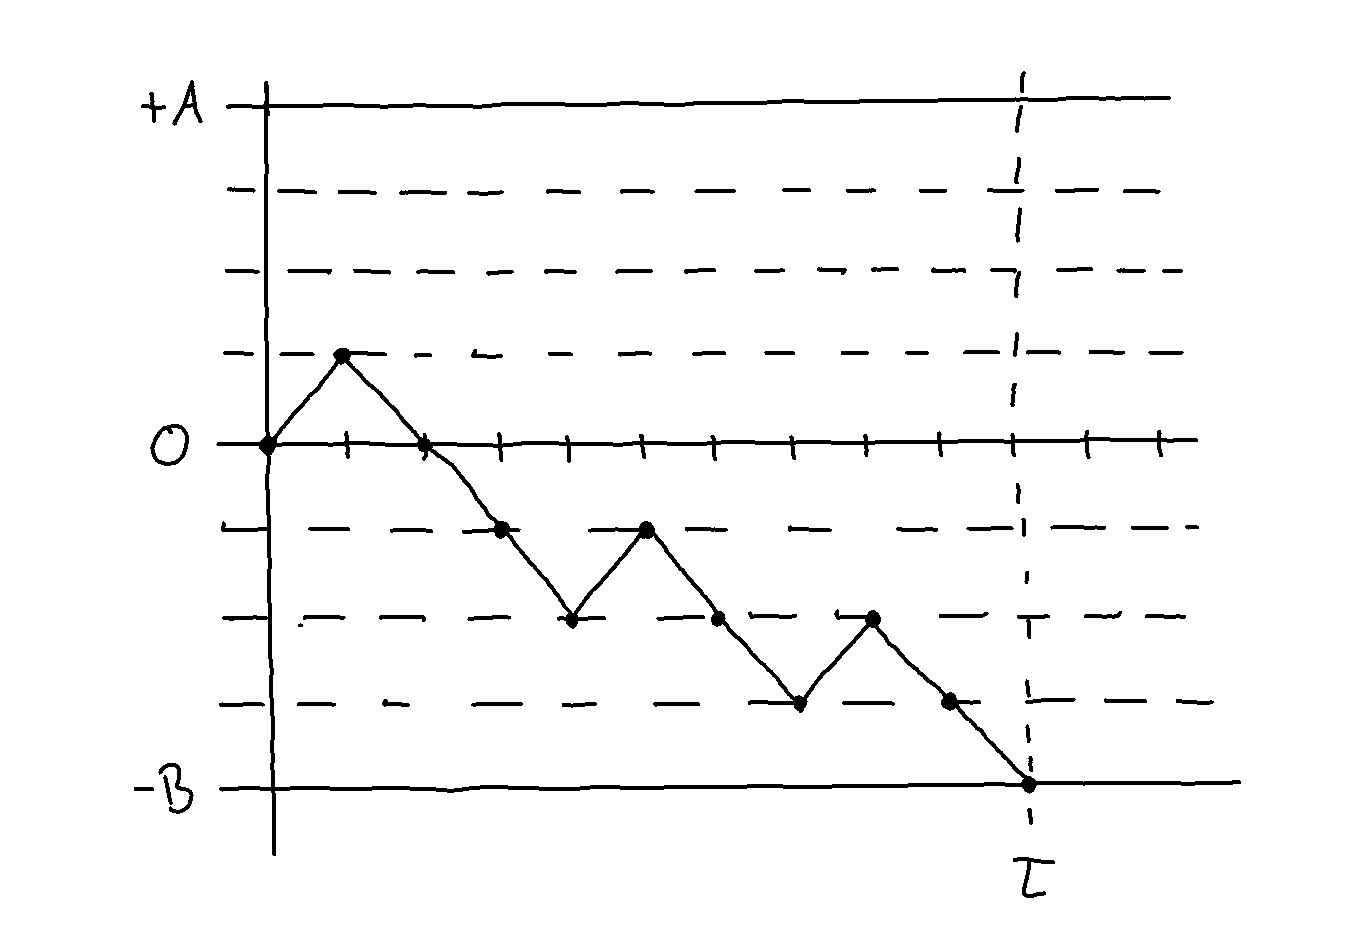
\includegraphics[width=0.75\textwidth]{./pics/Sketch0.png}
	\caption{Ein Random Walk, der eine Eintrittszeit erreicht}
	\label{AbbEintrittszeit}
\end{figure}
\enter
\underline{Fragen:} 
\begin{enumerate}
\item $\P\big( X\text{ erreicht }+A\text{ vor }-B\big)$?
\item $\E\big[\text{ Wartezeit bis }X\text{ Wert }+A\text{ vor }-B\text{ erreicht }\big]$?
\end{enumerate}
Definiere Stoppzeiten 
\begin{align*}
\tau_A&:=\min\big\lbrace n\in\N_0:X_n=+A\big\rbrace\text{ ``Erste Treffzeit von $A$''}\\
\tau_B&:=\min\big\lbrace n\in\N_0:X_n=-B\big\rbrace\text{ ``Erste Treffzeit von $-B$''}\\
\tau&:=\tau_A\wedge\tau_B\text{ ``Erste Treffzeit von $A$ oder $B$``}
\end{align*}
Es gilt $\P[\tau<\infty]=1$  und $\E[\tau]<\infty$ (überprüfen wir beides am Schluss).\\

\underline{Zu Frage 1:}
\begin{align*}
p:=\P\big( X\text{ erreicht }A\text{ vor }-B\big)=\P\big(\tau_A\leq\tau_B\big)
\end{align*}
$X$ ist Martingal, $\big|X_{\tau\wedge n}\big|\leq\max\lbrace A,B\rbrace$. Somit folgt aus Theorem \ref{theorem3.3}:
\begin{align*}
\E\big[X_\tau\big]=\E\big[X_0\big]=0
\end{align*}
Andererseits: 
\begin{align*}
\E\big[X_\tau\big]&=\E\Big[\underbrace{X_{\tau_A}}_{=A}\cdot\indi_{\lbrace\tau_A<\tau_B\rbrace}+\underbrace{X_{\tau_B}}_{=-B}\cdot\indi_{\lbrace\tau_A>\tau_B\rbrace}\Big]\\
&=A\cdot\P\big(\tau_A<\tau_B\big)-B\cdot\P\big(\tau_A>\tau_B\big)\\
&=A\cdot p-B\cdot(1-p)\\
&=p\cdot(A+B)-B\\
&\implies
p=\frac{B}{A+B}
\end{align*}
und somit:
\begin{align*}
\P\big(X\text{ trifft }+A\text{ vor }-B\big)&=\frac{B}{A+B}\\
\P\big(X\text{ trifft }-B\text{ vor }+A\big)&=\frac{A}{A+B}\\
\end{align*}

\underline{Zu Frage 2:}\\
Berechne Kompensator $\langle X\rangle_n$:
\begin{align*}
\E\Big[\underbrace{(X_n-X_{n-1})^2}_{=1}~\Big|~\F_{n-1}\big]=\langle X\rangle_n-\langle X\rangle_{n-1}\\
\implies \langle X\rangle_n=n
\implies M_n=X_n^2-n\text{ ist Martingal}
\end{align*}
Da
\begin{align*}
\big|M_{n\wedge\tau}\big|&\leq
\max\lbrace A^2,B^2\rbrace+\tau
\end{align*}
eine integrierbare (weil $\E[\tau]<\infty$) obere Schranke ist, folgt mit majorierter Konvergenz:
\begin{align*}
\E[M_\tau]&=\limn\E\big[M_{\tau\wedge n}\big]\stackeq{\ref{theorem3.2}}
\E[M_0]=0
\end{align*}
Andererseits:
\begin{align*}
\E[M_\tau]
&=\E\big[X_\tau^2-\tau\big]\\
&=\E\Big[\underbrace{X^2_{\tau_A}}_{=A^2}\cdot\indi_{\lbrace\tau_A<\tau_B\rbrace}+\underbrace{X^2_{\tau_B}}_{=B^2}\cdot\indi_{\lbrace\tau_A>\tau_B\rbrace}\Big] - \E[\tau]\\
&=A^2\cdot\P\big(\tau_A<\tau_B\big)+B^2\cdot\P\big(\tau_B<\tau_A\big)-\E[\tau]\\
&=A^2\cdot\frac{B}{A+B}+B^2\cdot\frac{A}{A+B}-\E[\tau]\\
&=\frac{A^2\cdot B + B^2 \cdot A}{A+B}-\E[\tau]\\
&=A\cdot B-\E[\tau]\\
&\implies
\E[\tau]=A\cdot B
\end{align*}
Also ist $E\big[\text{Wartezeit bis }X\text{ den Wert }+A\text{ oder }-B\text{ erreicht}\big]=A\cdot B$.\\

\underline{Überprüfen von $P(\tau<\infty)=1$:}\\
Definiere Ereignisse
\begin{align*}
\E_k:=\Big\lbrace\omega\in\Omega:X(\omega)\text{ steigt monoton für }k\cdot(A+B)\leq n<(k+1)\cdot(A+B)\Big\rbrace~~\forall k\in\N_0
\end{align*}
%TODO Hier Skizze einfügen
Es gilt
\begin{align*}
\omega\in E_k\implies \tau(\omega)\leq(k+1)\cdot(A+B)
\end{align*}
Kontraposition:
\begin{align*}
\tau(\omega)>(k+1)\cdot(A+B)\implies\omega\not\in E_k
\end{align*}
Außerdem: $E_1,E_2,\ldots$ sind unabhängig mit $\P(E_1)=\P(E_2)=\ldots$ und
\begin{align*}
\P(E_1)=2^{-(A+B)}\in(0,1).
\end{align*}
Somit folgt
\begin{align*}
\P\big(\tau>n\cdot(A+B)\big)&=\P\left(\bigcap\limits_{k=0}^n\big\lbrace\tau > k\cdot (A+B)\big\rbrace\right)\\
&\leq\P\left(\bigcap\limits_{k=0}^{n-1} E_k^C\right)\\
&=\Big(1-\P(E_1)\Big)^n\stackrel{n\to\infty}{\longrightarrow}0\\
\P(\tau=\infty)&\leq\underbrace{\P\big(\tau> n\cdot(A+B)\big)}_{\stackrel{n\to\infty}{\longrightarrow}0}\qquad\forall n\in\N_0\\
&\implies
\P(\tau<\infty)=1
\end{align*}
\end{beisp}





% This work is licensed under the Creative Commons
% Attribution-NonCommercial-ShareAlike 4.0 International License. To view a copy
% of this license, visit http://creativecommons.org/licenses/by-nc-sa/4.0/ or
% send a letter to Creative Commons, PO Box 1866, Mountain View, CA 94042, USA.

\chapter{Martingalkonvergenz und gleichgradige Integrierbarkeit} %4

\section{Martingalkonvergenz} %4.1
\setcounter{section}{4} %fix numbering
\underline{Vorüberlegung:} Sei $(a_n)_{n\in\N}\subseteq\R$ deterministische Folge in $\R$.
\begin{itemize}
	\item $\liminf\limits_{n\to\infty} a_n$ und $\limsup\limits_{n\to\infty} a_n$ immer wohldefiniert mit Werten in $\overline{\R}:=\R\cup\lbrace\pm\infty\rbrace$
	\item Grenzwert $\limn a_n$ existiert in $\overline{\R}$
	\begin{align*}
		\Longleftrightarrow\liminf\limits_{n\to\infty} a_n=\limsup\limits_{n\to\infty} a_n
	\end{align*}
	\item Mit Kontraposition gilt also 
	\begin{align*}
		&\lim a_n\text{ existiert \ul{nicht} in }\overline{\R}\\
		&\Longleftrightarrow\liminf\limits_{n\to\infty} a_n<\limsup\limits_{n\to\infty} a_n\\
		&\Longleftrightarrow
		\exists p,q\in\Q\mit p<q:\liminf\limits_{n\to\infty} a_n<p<q<\limsup\limits_{n\to\infty} a_n\\
		&\Longleftrightarrow
		\exists p,q\in\Q\mit p<q:\\
		&\qquad(a_n)_{n\in\N}\text{ unendlich oft den Streifen }[p,q]\times\N\text{ ``aufsteigend'' überquert}\\
		&\Longleftrightarrow
		\exists p,q\in\Q\mit p<q:U[p,q]=\infty
	\end{align*}
	wobei $U[p,q]$ die \textbf{upcrossings} (aufsteigende Überquerungen) des Streifens $[p,q]\times\N$ bezeichnet.
\end{itemize}

\begin{figure}[ht!]
	\begin{center}
		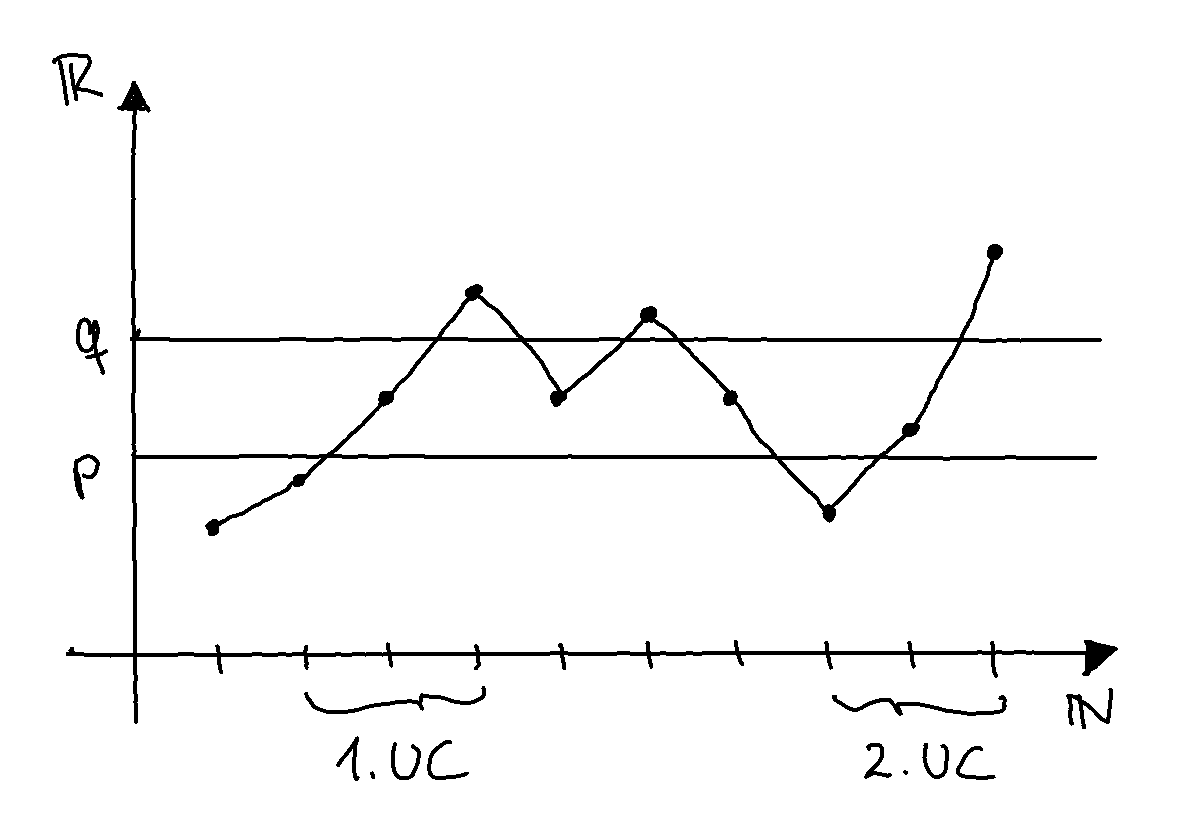
\includegraphics[width=0.75\textwidth]{./pics/Sketch2.png}
		\caption{Beispiel für Upcrossings}
		\label{AbbUpcrossing}
	\end{center}
\end{figure}

\begin{defi}
	Sei $(X_n)_{n\in\N}$ ein adaptierter stochastischer Prozess und $p,q\in\R$ , $p<q$ , $N\in\N$.
	Setze % Die einzelnen $..$ Umgebungen sind hier wichtig, sonst passiert ein Zeilenumbruch inmitten der Matheumgebung
	\begin{align*}
		U_N[p,q]:=\max\left\{ k\in\N_0\left|
		\begin{array}{c}
			\exists\text{ Stoppzeiten }0<\sigma_1<\tau_1<\sigma_2<\tau_2<\ldots<\tau_k\le N\\
			\forall i\in\lbrace 1,\ldots,k\rbrace: X_{\sigma_i}<p \text{ und } X_{\tau_i}>q
		\end{array}\right.\right\} % hier Wort "und" da sonst Verwirrung mit minimum
	\end{align*}
	$U_N[p,q]$ ist die Anzahl der \textbf{Upcrossings} von $[p,q]\times\lbrace0,1,\ldots,N\rbrace$ durch $(X_n)_{n\in\N}$ und 
	\begin{align*}
		U[p,q]=\limsup\limits_{n\to\infty} U_n[p,q]
	\end{align*}
	die Anzahl der \textbf{Upcrossings} von $[p,q]\times\N$.
\end{defi}

\begin{lemma}[Doob's Upcrossing Lemma]\enter\label{lemma4.1DoobsUpcrossingLemma}
	Sei $(X_n)_{n\in\N}$ Sub-Martingal und $p,q\in\R\mit p<q$. Dann gilt:
	\begin{align*}
		\E\big[U_N[p,q]\big]&\leq\frac{\E\big[(X_N-p)^+\big]}{q-p}\qquad\forall N\in\N
	\end{align*}
\end{lemma}

\begin{bemerkung}
	\textbf{Positivteil} und \textbf{Negativteil} einer Zufallsvariblen $X$ ist definiert als
	\begin{align*}
		X^+(\omega):=\max\big\lbrace X(\omega),0\big\rbrace
		\qquad\text{ und }\qquad
		X^-(\omega):=-\min\big\lbrace X(\omega),0\big\rbrace
	\end{align*}
	Es gilt $X=X^+-X^-$ und $|X|=X^++X^-$.
\end{bemerkung}

\begin{proof}
	Setze der Kürze halber $k(\omega):=U_N[p,q](\omega)$. Klarerweise ist $k\leq N$. Definiere
	\begin{align*}
		\tau_0&:=0\\
		\sigma_j&:=\min\big\lbrace k\geq \tau_{j-1}:X_k<p\big\rbrace\wedge N\text{ ``Erstaustrittszeit''}\\
		\tau_j&:=\max\big\lbrace k\geq\sigma_j:X_k>q\big\rbrace\wedge N
	\end{align*}
	d. h. $\tau_0<\overbrace{\sigma_1<\tau_1}^{\text{1. Upcrossing}}<\overbrace{\sigma_2<\ldots}^{\text{2. Upcrossing}}\ldots<\tau_k$ und
	$\tau_{k+1}=\sigma_{k+1}=\tau_{k+2}=\ldots=\tau_N=N$. Es gilt:
	\begin{align}\label{eqProof4.1.1Stern}\tag{$\ast$}
		(q-p)\cdot U_N[p,q] &\leq
		\overbrace{\underbrace{(X_{\tau_1}-p)}_{>q-p}+\underbrace{(X_{\tau_2}-X_{\sigma_2})}_{>q-p}+\ldots+\underbrace{(X_{\tau_k}-X_{\sigma_k})}_{>q-p}}	^{U_N[p,q]\text{ Summanden}}
	\end{align}
	Außerdem gilt
	\begin{align}\label{eqProof4.1.1ZweiStern}\tag{$\ast\ast$}
		\min\lbrace X_N-p,0\rbrace&\leq X_N-X_{\sigma_{k+1}},
	\end{align}
	denn: 
	\begin{align*}
		X_N-p<0&\implies X_{\sigma_{k+1}}<p&&\implies X_N-p\leq X_{\sigma_{k+1}}-p\\
		X_N-p\geq0 &\implies \sigma_{k+1}=N&&\implies X_N- X_{\sigma_{k+1}}=0
	\end{align*}
	Addiere von \eqref{eqProof4.1.1Stern} auf \eqref{eqProof4.1.1ZweiStern}
	\begin{align*}
		(q-p)\cdot U_N[p,q]+\underbrace{\min\lbrace X_N-p,0\rbrace}_{\stackeq{\text{def}}-(X_N-p)^-}\leq (X_{\tau_1}-p) + \sum_{i=2}^N (X_{\tau_i} - X_{\sigma_i})
	\end{align*}
	Bilden von Erwartungswert und Umordnen der Summe liefert
	\begin{align*}
		(q-p)\cdot\E\big[U_N[p,q]\big]-\E\big[(X_N-p)^-\big]
		&\leq\E[X_N]-\left(p+\sum\limits_{j=1}^{N-1}\Big(\underbrace{\E\big[X_{\sigma_{j+1}}\big]-\E\big[X_{\tau_j}\big]}_{\geq 0\text{, wegen Theorem \ref{theorem3.4}}}\Big)\right)\\
		&\leq\E\big[(X_N-p)\big]\\
		\implies
		(q-p)\cdot\E\big[U_N[p,q]\big]&\leq\E\big[(X_N-p)+(X_N-p)^-\big]\\
		&=\E\big[(X_N-p)^+\big]
	\end{align*}
\end{proof}

\begin{theorem}[Martingalkonvergenz]\label{theorem4.2Martingalkonvergenz}\enter
	Sei $(X_n)_{n\in\N}$ ein Submartingal mit $\sup\limits_{n\in\N}\E[X_n^+]<\infty$. Dann gilt:
	\begin{align*}
		\exists X_\infty\in L_1(\Omega,\A,\P):\limn X_n=X_\infty\text{ fast sicher}
	\end{align*}
\end{theorem}

\begin{proof}
	Zunächst zeigen wir den Satz für $X_\infty$ mit Werten in $\overline{\R}$. Mit Vorüberlegung (zu Beginn des Kapitels) reicht es zu zeigen:
	\begin{align*}
		\P\big(U[p,q]=\infty\big)=0\qquad\forall p,q\in\Q\mit p<q
	\end{align*}
	denn:
	\begin{align*}
		\P\left(\limn X_n\text{ exisitiert nicht in }\overline{\R}\right)
		&=\P\left(\bigcup\limits_{\begin{subarray}{c}p,q\in\Q\\ p<q\end{subarray}}\big\lbrace U[p,q]=\infty\big\rbrace\right)\\
		&\leq\sum\limits_{p,q\in\Q}\P\big(U[p,q]=\infty\big)\\
		&=0
	\end{align*}
	Mit Lemma \ref{lemma4.1DoobsUpcrossingLemma} gilt:
	\begin{align*}
		\E\big[U[p,q]\big]
		\overset{\text{Mono}}&=
		\limsup\limits_{N\to\infty}\E\big[U_N[p,q]\big]\\
		\overset{\ref{lemma4.1DoobsUpcrossingLemma}}&{\leq}
		\limsup\limits_{N\to\infty}\frac{\E\big[(X_N-p)^+\big]}{q-p}\\
		&\leq\limsup\limits_{N\to\infty}\frac{\E[X_N^+]+p}{q-p}\\
		\overset{\text{Vor}}&{<}
		\infty\qquad\forall p,q\in\Q\mit p<q\\
		\implies
		\P\big(U[p,q]<\infty\big)&=1
	\end{align*}
	Also existiert $X_\infty$ mit Werten in $\overline{\R}$ und $\limn X_n=X_\infty$ fast sicher.\\
	Noch zu zeigen: $X_\infty\in(-\infty,\infty)$ fast sicher und $\E\big[|X_\infty|\big]<\infty$.\\
	Mit $|X|=2\cdot X^+-X$ gilt
	\begin{align*}
		\E\left[\limn|X_n|\right]
		\overset{\text{Fatou}}&{\leq}
		\liminf\limits_{n\to\infty}\E\big[|X_n|\big]\\
		&=\liminf\limits_{n\to\infty}\Big(2\cdot\E[X_n^+]-\underbrace{\E[X_n]}_{\stackrel{\text{SubM}}{\geq}\E[X_0]}\Big)\\
		&\leq
		2\cdot\underbrace{\sup\limits_{n\in\N}\E[X_n^+]}_{\stackrel{\text{Vor}}{<}\infty}-\E[X_0]\\
		&<\infty\\
		\implies\E\big[|X_\infty|\big]&<\infty
	\end{align*}
	Insbesondere gilt $X_\infty\in(-\infty,\infty)$.
\end{proof}

\begin{bemerkung}
	Aus Theorem \ref{theorem4.2Martingalkonvergenz} folgt \ul{nicht} die stärkere $L_1$-Konvergenz\\ $\E\big[|X_n-X_\infty|\big]\longrightarrow0$.\\
	Gegenbeispiel: siehe Übungsblatt 2, Aufgabe 3
	\begin{align*}
		M_n^u:=\exp\left(u\cdot X_n-\frac{n\cdot\sigma^2\cdot u^2}{2}\right)\mit X_n=\xi_1+\ldots+\xi_n\text{ Random-Walk},\xi\sim\mathcal{N}(0,\sigma^2)
	\end{align*}
	In der Übung wurde gezeigt:
	\begin{align*}
		\limn M_n=0\text{ fast sicher}\qquad\forall u\neq0
	\end{align*}
	aber
	\begin{align*}
		\E\big[|M_n^u-0|\big]=\E[M_n^u]=1 \text{ keine $L_1$-Konvergenz!}
	\end{align*}
\end{bemerkung}

\begin{beisp}[Wählermodell]\enter
	Wähle $L,d\in\N$. Betrachte $L^d$ Individuen auf dem regelmäßigen Gitter\\ $\Lambda:=\lbrace 0,1,\ldots,L-1\rbrace^d$
	\begin{figure}[!ht]
		\begin{center}
			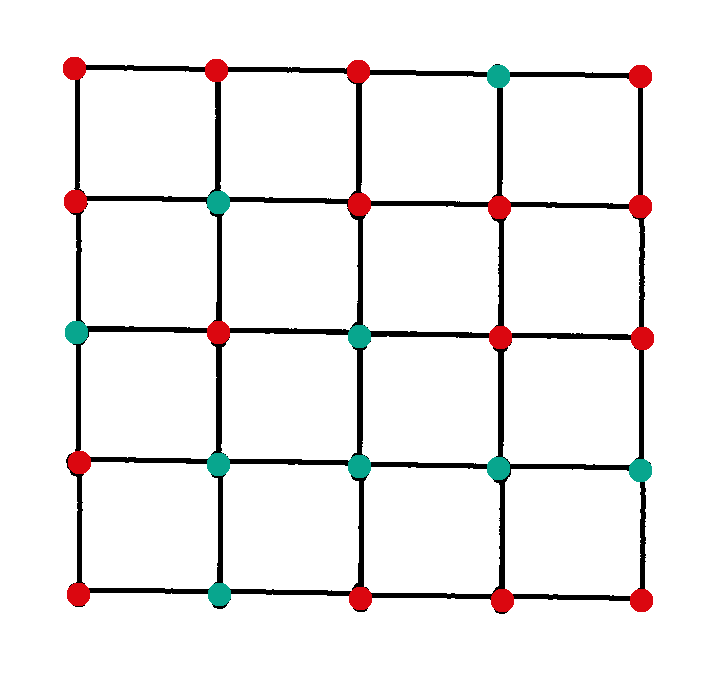
\includegraphics[width=0.5\textwidth]{./pics/Sketch1.png}
			\caption{Individuen-Gitter für $d=2$ und $L=4$}
			\label{AbbGitter}
		\end{center}
	\end{figure}

	Jedes Individuum hat Meinung in $\lbrace0,1\rbrace$, also dafür oder dagegen. Zustand des Kollektivs:
	$x\in\lbrace0,1\rbrace^{\Lambda}=\big\lbrace f:\Lambda\to\lbrace 0,1\rbrace\big\rbrace=\lbrace0,1\rbrace^{L^d}$\nl
	\ul{Meinungsbildungsprozess:} Zu jedem Zeitpunkt $n\in\N_0$ übernimmt ein (zufällig ausgewähltes) Individuum $I_n$ die Meinung eines (zufällig ausgewählten) Nachbarn $I_n+N_n$. 
	(Konvention: Es gibt keinen Rand, es wird modulo $L$ gerechnet.)\nl
	\ul{Mathematische Formulierung}: $(I_n,N_n)_{n\in\N_0}$ iid mit 
	\begin{itemize}
		\item $I_n$ $\ldots$ gleichverteilt auf dem Gitter $\Lambda$
		\item $N_n$ $\ldots$ gleichverteilt auf $(\pm e_i)_{i\in\lbrace1,\ldots,d\rbrace}$
	\end{itemize}
	\ul{Meinungsprozess:} $X_n$ ist eine Folge von Zufallsvariablen mit Werten in Zustandsraum $\lbrace0,1\rbrace^\Lambda$ mit
	\begin{align*}
		X_n(i)=\left\lbrace\begin{array}{cl}
			X_{n-1}(i), &\falls i\neq I_n\\
			X_{n-1}(i+N_n),&\falls i=I_n
		\end{array}\right.\qquad\forall i\in\Lambda
	\end{align*}
	\ul{Fragen:}
	\begin{itemize}
		\item Langzeitverhalten?
		\item Tritt Konsens ein?
	\end{itemize}
	Definiere das Martingal $M_n:=$ ``Anzahl der Individuen mit Meinung 1``, also
	\begin{align*}
		M_n:=\sum\limits_{i\in\Lambda} X_n(i),\qquad \F_n:=\sigma\Big((I_k,N_k))_{k\in\lbrace1,\ldots,n\rbrace}\Big)
	\end{align*}
	\ul{Behauptung:} $M_n$ ist Martingal.
	\begin{itemize}
		\item Adaptiertheit: Klar nach Definition von $\F_n$
		\item Integrierbarkeit: $M_n$ ist sogar beschränkt: $0\leq M_n\leq L^d$
		\item Martingal-Eigenschaft:
		\begin{align*}
			&M_n-M_{n-1}
			=\underbrace{X_{n-1}(I_n+N_n)}_{\text{vom Nachbarn übernommen}}-\underbrace{X_{n-1}(I_n)}_{\text{alte Meinung}}\\
			\implies&\E\big[M_n-M_{n-1}~\big|~\F_{n-1}\big]\\
			&=\E\big[X_{n-1}(I_n+N_n)-X_{n-1}(I_n)~\big|~\F_{n-1}\big]\\
			&=\sum\limits_{i\in\Lambda} X_{n-1}(i)\cdot\P\big(i=\underbrace{I_n+N_n)~\big|~\F_{n-1}}_{\unab}\big)-X_{n-1}(i)\cdot\P\big(\underbrace{i=I_n~\big|~\F_{n-1}}_{\unab}\big)\\
			&=\sum\limits_{i\in\Lambda} X_{n-1}(i)\cdot\Big(\underbrace{\P(i=I_n+N_n)}_{=L^{-d}}-\underbrace{\P(I_n=i)}_{=L^{-d}}\Big)\\
			&=0
		\end{align*}
	\end{itemize}
	Folglich ist $(M_n)$ ein beschränktes Martingal und somit existiert gemäß Theorem \ref{theorem4.2Martingalkonvergenz}
	$M_\infty\mit\limn M_n=M_\infty$ (Achtung extra Annahme: und in $L_1\implies\E[M_\infty]=\E[M_0]$).\nl
	\ul{Weitere Behauptung:} $M_\infty\in\lbrace 0,L^d\rbrace$, d.h. im Grenzwert gibt es nur extreme Zustände (Konsens).\nl
	\ul{Vorüberlegung:} Sei $x\in\lbrace0,1\rbrace^{\Lambda}$ \ul{kein} extremer Zustand, d. h. es existieren Nachbarn $i,j$ mit $X_n(i)\neq X_n(j)$.
	\begin{align}
		\P(X_n\neq X_{n-1}~|~X_{n-1}=x)\nonumber
		&\geq \P\Big(\Big\lbrace I_n=i\Big\rbrace \cap \Big\lbrace I_n+N_n=j~(\text{mod } L)\Big\rbrace\Big)\\
		&=\P\Big(\underbrace{\Big\lbrace I_n=i\Big\rbrace \cap\Big\lbrace N_n=i-j~(\text{mod  }L)\Big\rbrace}_{\unab}\Big)\nonumber\\
		&=\P\big(I_n=i\big)\cdot\P\big(N_n=i-j~(\text{mod  }L)\big)\nonumber\\
		&=L^{-d}\cdot\frac{1}{2\cdot d}\label{eqExampleWaehlermodellStern}\tag{$\ast$}
	\end{align}
	Der Kompensator $\langle M\rangle_n$ erfüllt
	\begin{align*}
		(M_n-M_0)^2-\langle M\rangle_n\text{ ist Martingal}\\
		\implies
		\E\big[\langle M\rangle_n\big]=\E\left[(M_n-M_0)^2\right]
	\end{align*}
	Andererseits gilt:
	\begin{align*}
		\langle M\rangle_n 
		&=\sum\limits_{k=1}^n\E\left[\left.\underbrace{(M_k-M_{k-1})^2}_{\in\lbrace0,1\rbrace}~\right|~\F_{k-1}\right]\\
		&=\sum\limits_{k=1}^n0 \cdot \P\big(X_k= X_{k-1}~\big|~\F_{k-1}\big)+ 1 \cdot \P\big(X_k\neq X_{k-1}~\big|~\F_{k-1}\big)\\
		%\Rightarrow
		\E\big[\langle M\rangle_n\big]
		\overset{\eqref{Turmregel}}&=
		\sum\limits_{k=1}^n\P\big(X_k\neq X_{k-1}\big)\\
		&=\sum\limits_{k=1}^n\underbrace{\P\big(X_k\neq X_{k-1}~|~ M_{k-1} \in \{0,L^d\}\big)}_{\geq 0} + \P\big(\underbrace{X_k\neq X_{k-1}~|~ M_{k-1} \not\in \{0,L^d\}}_{\unab}\big)\\
		\overset{\eqref{eqExampleWaehlermodellStern}}&{\geq}
		\sum\limits_{k=1}^n L^{-d}\cdot\frac{1}{2\cdot d}\cdot\P\big(\underbrace{M_{k-1}\not\in\lbrace0,L^d\rbrace}_{=:A_{k-1}\text{ (kein extremer Zustand)}}\Big)
	\end{align*}
	Außerdem:
	\begin{align*}
		L^{2\cdot d}
		&\geq \E\left[(M_n-M_0)^2\right]\\
		&=\E\big[\langle M\rangle_n\big]\\
		&\geq L^{-d}\cdot\frac{1}{2\cdot d}\cdot\sum\limits_{k=1}^n\P(A_{k-1})\\
		\implies
		\sum\limits_{k=1}^n\P(A_{k-1})&\leq L^{3\cdot d}\cdot 2\cdot d<\infty
	\end{align*}

	Satz von Borel-Cantelli: Nur endlich viele Ereignisse $(A_k)_{k\in\N}$ treten ein, d.h.
	\begin{align*}
		&\exists N_0:\Omega\to\N:\forall n\geq N_0(\omega):\omega\not\in A_n\\
		&\implies M_n(\omega)\in\lbrace0,L^d\rbrace\qquad\forall N_0(\omega)\\
		&\implies M_\infty:=\limn M_n\text{ nimmt nur extreme Werte $\lbrace0,L^d\rbrace$ an!}
	\end{align*}
	Im Grenzwert tritt perfekter Konsens auf!
	\begin{align*}
		\P\big(M_\infty=L^d\big)&=L^{-d}\cdot\E[M_\infty]\stackeq{L_1\text{-Konv}} L^{-d}\cdot\E[M_0]\\
		\P(M_\infty=0)&=1-L^{-d}\cdot\E[M_0]
	\end{align*}
\end{beisp}

\setcounter{section}{1} %fix numbering
\section{Gleichgradige Integrierbarkeit (ggi)} %4.2
\setcounter{section}{4} %fix numbering
\ul{Ziel}: $L_1$-Konvergenz und Abschließbarkeit von Martingalen

\begin{defi}
	Sei $(X_i)_{i\in I}$ eine Familie von Zufallsvariablen. Setze
	\begin{align*}
		\rho(R):=\sup\limits_{i\in I}\E\Big[|X_i|\cdot\indi_{\lbrace |X_i|\geq R\rbrace}\Big]
	\end{align*}
	Die Familie $(X_i)_{i\in I}$ heißt \textbf{gleichgradig integrierbar (ggi)}
	\begin{align*}
		:\Longleftrightarrow\lim\limits_{R\to\infty}\rho(R)=0
	\end{align*}
	Interpretation: Masse in Verteilungsende verschwindet gleichmäßig für $R\to\infty$.
	\begin{figure}[!ht]
		\begin{center}
			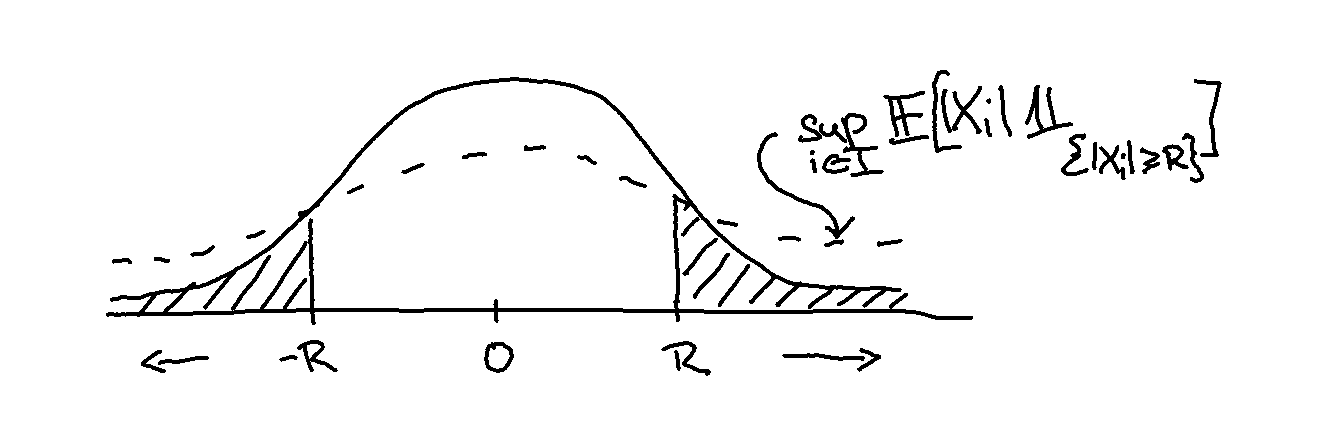
\includegraphics[width=\textwidth]{pics/Sketch3.png}
			\caption{Veranschaulichung von $\rho(R)$ aus der Definition von ggi}
			\label{AbbRhoGGI}
		\end{center}
	\end{figure}
\end{defi}

\setcounter{satz}{2}
\begin{lemma}\label{lemma4.3}
	Sei $X\in L_1(\Omega,\A,\P)$. Dann gilt:
	\begin{enumerate}[label=(\alph*)]
		\item $\lbrace X\rbrace$ ist ggi
		\item $\big\lbrace\E[X~|~\F]:\F\text{ ist Unter-$\sigma$-Algebra von }\A\big\rbrace$ ist ggi
	\end{enumerate}
\end{lemma}

\begin{bemerkung}
	Insbesondere gilt: Wenn $X$ Martingal ist, ist $(X_t)_{t\in[0,T]}$ ist ggi, ABER $(X_t)_{[t\geq0}$ im Allgemeinen nicht!
\end{bemerkung}

\begin{proof}
	\underline{Zeige (a):}\\
	Es gilt
	\begin{align*}
		|X|\cdot\indi_{\lbrace|X|\geq R\rbrace}\leq |X|
	\end{align*}
	Daher folgt mit dominierter Konvergenz:
	\begin{align*}
		\lim\limits_{R\to\infty}\rho(R)
		&=\lim\limits_{R\to\infty}\E\left[|X|\cdot\indi_{\lbrace |X|\geq R\rbrace}\right]
		\stackeq{\text{domKonv}}\E\left[|X|\cdot\lim\limits_{R\to\infty}\indi_{\lbrace|X|\geq R\rbrace}\right]
		=0
	\end{align*}
	\underline{Zeige (b):} $\F\subseteq\A$, $Y:=\E[X~|~F]$ Es gilt
	\begin{align*}
		|Y|&\leq\E\big[|X|~\big|~\F\big]\\
		\E\left[|Y|\cdot\indi_{\lbrace|Y|\geq R\rbrace}\right]
		&\leq\E\Big[\E\big[|X|~\big|~\F\big]\cdot\indi_{\lbrace |Y|\leq R\rbrace}\Big]
		\stackrel{\text{Tow}}{\leq}
		\E\left[|X|\cdot\indi_{\lbrace|Y|\geq R\rbrace}\right]
	\end{align*}
	Sei $K\geq0$.
	\begin{align*}
		\E\Big[|X|\cdot\indi_{\lbrace|Y|\geq R\rbrace}\Big]
		&=\underbrace{\E\big[|X|\cdot\indi_{\lbrace |Y|\geq R\rbrace}\cdot\indi_{\lbrace |X|>K\rbrace}\Big]}_{\leq\E\Big[|X|\cdot\indi_{\lbrace |X|\geq K\rbrace}\Big]}+
		\underbrace{\E\Big[|X|\cdot\indi_{\lbrace|Y|\geq R\rbrace}\cdot\indi_{\lbrace|X|<K\rbrace}\Big]}_{\leq|X|\cdot\P\big(|Y|\geq R\big)\stackrel{\text{Markov}}{\leq}\frac{K}{R}\cdot\E\big[|Y|\big]\leq\frac{K}{R}\cdot\E\big[|X|\big]}
	\end{align*}
	Insgesamt:
	\begin{align*}
		\rho(R)
		&\leq\E\Big[|X|\cdot\indi_{\lbrace|X|\geq R}\Big]+\frac{K}{R}\cdot\E\big[|X|\big]\qquad\forall K\geq0\\
		\implies
		\lim\limits_{R\to\infty}\rho(R)
		&\leq\E\Big[|X|\cdot\indi_{|X|\geq K\rbrace}\Big]\stackrel{K\to\infty}{\longrightarrow}0\\
		\implies \lim\limits_{R\to\infty}\rho(R)&=0
	\end{align*}
\end{proof}

\begin{theorem}[Hinreichende Bedigungen für ggi]\label{theorem4.4HinreichendeBeingungenFuerggi}\enter
	Sei $(X_i)_{i\in I}\subseteq L_1$ eine Familie von Zufallsvariablen. Dann gilt:
	\begin{enumerate}[label=(\alph*)]
		\item $\begin{aligned}
			\Big(\exists p>1:\sup\limits_{i\in I}\E\big[|X_i|^p\big]<\infty\Big)\implies (X_i)_{i\in I}\text{ ist ggi}
		\end{aligned}$
		\item $\begin{aligned}
			\Big(\exists Y\in L_1:\forall i\in I:|X_i|\leq Y\Big)\implies(X_i)_{i\in I}\text{ ist ggi}
		\end{aligned}$
	\end{enumerate}
\end{theorem}

\begin{proof}
	\underline{Zu (a):} Siehe Übung.\nl
	\underline{Zu (b):}
	\begin{align*}
		\rho(R)&=\E\Big[|X_i|\cdot\indi_{\lbrace |X_i|\geq R\rbrace}\Big] \\
		\overset{\text{Vor.}}&{\leq}
		\E\Big[|Y|\cdot\indi_{\lbrace |X_i|\geq R\rbrace}\Big] \\
		&\leq\E\Big[|Y|\cdot\indi_{\lbrace |Y|\geq R\rbrace}\Big]\\
		&\text{denn: }\big\lbrace |X_i|\geq R\big\rbrace\subseteq\big\lbrace|Y|\geq R\big\rbrace\qquad\forall i\in I\\
		\implies
		\rho(R)
		&\leq\E\Big[|Y|\cdot\indi_{\lbrace |Y|\geq R\rbrace}\Big]\underset{\ref{lemma4.3} (a)}{\overset{R\to\infty}{\longrightarrow}}0
	\end{align*}
\end{proof}

\begin{theorem}\label{theorem4.5}
	Sei $(X_n)_{n\in\N}$ ggi und $\limn X_n=:X_\infty$ f.s.\\
	Dann gilt $L_1$-Konvergenz:
	\begin{align*}
		\E\big[|X_n-X_\infty|\big]\stackrel{n\to\infty}{\longrightarrow}0
		\qquad\text{d.h.}\qquad
		X_n\stackrel{L_1}{\longrightarrow} X_\infty
	\end{align*}
\end{theorem}

\begin{bemerkung}
	Merke: Fast sichere Konvergenz + ggi $\implies L_1$-Konvergenz
\end{bemerkung}

\begin{proof}
	Schreibe $X:=X_\infty$. Es gilt
	\begin{align*}
		\E\Big[|X|\cdot\indi_{\lbrace |X|\geq R\rbrace}\Big]
		&\stackrel{\text{Fatou}}{\leq}
		\liminf\limits_{n\to\infty}\E\Big[|X_n|\cdot\indi_{\lbrace |X_n|\geq R\rbrace}\Big]
		\stackrel{\text{ggi}}{\leq}
		\rho(R)
	\end{align*}
	Folglich
	\begin{align*}
		\E\big[|X|\big]&=\underbrace{\E\Big[|X|\cdot\indi_{\lbrace |X|< R\rbrace}\Big]}_{\leq R}+\underbrace{\E\Big[|X|\cdot\indi_{\lbrace |X|\geq R\rbrace}\Big]}_{\leq\rho(R)}
		\leq R+\rho(R)<\infty\qquad\forall R\geq0
	\end{align*}
	Also $X\in L_1$. Nun schätzen wir noch die Differenz ab:
	\begin{align*}
		|X_n-X|
		\overset{\triangle\text{-Ungl.}}&{\leq}
		\underbrace{|X_n-X|\cdot\indi_{\lbrace |X|\geq R\rbrace}}_{\leq R+|X|}+\underbrace{|X_n|\cdot\indi_{\lbrace |X_n|\geq R\rbrace}}_{\E[\cdot]\leq\rho(R)}+\underbrace{|X|\cdot\indi_{\lbrace |X_n|\geq R\rbrace}}_{\E[\cdot]\leq\rho(R)}\\
		&\implies
		\limn\E\big[|X_n-X|\big]
		\stackrel{\text{dom.Konv.}}{\leq}
		\underbrace{2\cdot\rho(R)}_{\stackrel{R\to\infty}{\longrightarrow}0}\qquad\forall R\geq0\\
		&\implies\limn\E\big[|X_n-X|\big]=0
	\end{align*}
\end{proof}

\begin{theorem}[$L_1$-Konvergenz von Martingalen]\label{theorem4.6L1KonvergenzVonMartingalen}\enter
	Sei $(X_n)_{n\in\N_0}$ ein $(\F_n)_{n\in\N_0}$-Martingal. Dann sind äquivalent:
	\begin{enumerate}[label=(\alph*)]
		\item $\begin{aligned}
			\exists X_\infty\in L_1(\F_\infty,\P):\E\big[|X_n-X_\infty|\big]\stackrel{n\to\infty}{\longrightarrow}0
		\end{aligned}$ ($L_1$-Konvergenz)
		\item $\begin{aligned}
			\exists X_\infty\in L_1(\F_\infty,\P):\forall n\in\N_0: X_n=\E\big[X_\infty~\big|~\F_n\big]
		\end{aligned}$ (Abschließbarkeit)
		\item $\begin{aligned}
			(X_n)_{n\in\N_0}
		\end{aligned}$ ist ggi
	\end{enumerate}
\end{theorem}

\begin{proof}
	\underline{Zeige (a) $\implies$ (b):} Sei $k\leq n$.
	\begin{align*}
		\E\Big[\big|X_k-\E[X_\infty~|~\F_k]\big|\Big]
		\overset{\text{MG}}&=
		\E\Big[\big|\E[X_n~|~\F_k]-\E[X_\infty~|~\F_k]\big|\Big]\\
		\overset{\text{\eqref{Turmregel}+Kontr}}&{\leq}
		\E\big[|X_n-X_\infty|\big]\stackrelnew{\text{(a)}}{n\to\infty}{\longrightarrow}0\\
		\implies X_k&=\E[X_\infty~|~\F_k]\qquad\forall k\in\N_0
	\end{align*}

	\underline{Zeige (b) $\implies$ (c):}\\
	Folgt aus Lemma \ref{lemma4.3} (b).\nl
	\underline{Zeige (c) $\implies$ (a):}
	\begin{align*}
		(X_n)_{n\in\N}\text{ ggi }&\implies\sup\limits_{n\in\N_0}\E\big[|X_n|\big]\leq R+\rho(R)<\infty\\
		&\stackrel{\ref{theorem4.2Martingalkonvergenz}}{\implies}
		\exists X_\infty\in L_1(\F_\infty,\P):\limn X_n=X_\infty\text{ f.s.}\\
		&\stackrel{\ref{theorem4.5}}{\implies}
		\limn\E\big[|X_n-X_\infty|\big]=0
	\end{align*}
\end{proof}

%\listoffigures 
%\listoftables
%\bibliography{literatur}


\end{document}
